\documentclass[
 paper=A4,pagesize=automedia,fontsize=12pt,
 BCOR=15mm,DIV=22,
 twoside,headinclude,footinclude=false,
 ngerman,%fleqn,            % fleqn = linksbündige Ausrichtung von Formeln
 bibtotocnumbered,          % Literaturverz. im Inhaltsverz. eintragen
 liststotoc,                % Abbildungsverz. im Inhaltsverz. eintragen
 listsleft,                 % Abbildungsverz. an der längsten Nummer ausrichten
 pointlessnumbers,          % kein Punkt nach Überschriftsnummerierung
 cleardoublepage=empty      % Vakatseiten ohne Paginierung
]{scrartcl}
\setlength\parindent{0em}

% Kodierung, Schrift und Sprache auswählen
\usepackage[utf8]{inputenc}
\usepackage[T1]{fontenc}
\usepackage[english]{babel}


%% damit man Text aus dem PDF korrekt rauskopieren kann
%\usepackage{cmap}
% Layout: Kopf-/Fußzeilen, anderthalbfacher Zeilenabstand
\usepackage{scrpage2} \pagestyle{scrheadings}
                      \clearscrheadfoot
                      \ihead{\headmark}\ohead{\pagemark}
                      \automark[subsection]{section}
                      \setheadsepline{0.5pt}
\usepackage{setspace} \onehalfspacing
%\deffootnote{1em}{1em}{\textsuperscript{\thefootnotemark }}
% Grafiken, Tabellen, Mathematikumgebungen
\usepackage{graphicx,xcolor}
\usepackage{tabularx}
\usepackage{amsmath,amsfonts,amssymb}
% Darstellung von Fließumgebungen
\usepackage{flafter,afterpage}
\usepackage[section]{placeins}
\usepackage[margin=8mm,font=small,labelfont=bf,format=plain]{caption}
\usepackage[margin=8mm,font=small,labelfont=bf,format=plain]{subcaption}

\numberwithin{equation}{section}
\numberwithin{figure}{section}
\numberwithin{table}{section}

%%%%%%%%%%%%%%%%%%%%%%%%%%%%%%%%%%%%%%%%%%%%%%%%%%%%%%%%%%%%%%%%%%%%%%%%%%%%%%%%
% Ab hier ist Platz für eigene Ergänzungen (Pakete, Befehle, etc.)

% hyperlink table of contents
\usepackage[colorlinks=true,linkcolor=black]{hyperref}
% double horizontal lines in tables
\usepackage{hhline}
% fat vertical lines for tabulars
\usepackage{array}
\newcolumntype{?}{!{\vrule width 2pt}} 
% fat vertical lines for tabulars
\makeatletter
\def\hlinewd#1{%
\noalign{\ifnum0=`}\fi\hrule \@height #1 %
\futurelet\reserved@a\@xhline}
\makeatother 
% to assign tables and figures in the right place
\usepackage{float}
% Referenzen fürs Zitiern
\usepackage{cite}         
% Stil des Quellenverzeichnis     
\bibliographystyle{ieeetr}    
% Package for nice seperation of number and unit
\usepackage[]{units}
% Package for code extracts
\usepackage{listings}
\lstset{breaklines=true,
  breakatwhitespace=true,
  stepnumber=1,
  basicstyle=\ttfamily\footnotesize,
  commentstyle=\ttfamily,
  prebreak={\textbackslash},
  breakindent=10pt,
  breakautoindent=false,
  showspaces=false,
  showstringspaces=false,
  frame=single,
  abovecaptionskip=0em,
  aboveskip=1.4em,
  belowcaptionskip=0.5em,
  belowskip=1em,
  keywordstyle=\ttfamily,
}
\definecolor{light}{RGB}{245,245,245}
\lstdefinestyle{Mybash}{
  language=bash,
  backgroundcolor=\color{light}
}
\lstdefinestyle{MyMathematica}{
  language=Mathematica,
  backgroundcolor=\color{light}
}

\lstdefinestyle{MyMathematicaOutput}{
  language=Mathematica
}
\lstdefinestyle{Mycpp}{
  language=C++,
  backgroundcolor=\color{light}
}
% diagonal separtion in table
\usepackage{diagbox}

% comment within a line
\newcommand{\ignore}[1]{}


% Differential quotients
\newcommand{\tdfrac} [2]{\ensuremath{\frac{\mathrm{d}   #1}{\mathrm{d} {#2}}}}%
\newcommand{\tddfrac}[2]{\ensuremath{\frac{\mathrm{d}^2 #1}{\mathrm{d} {#2}^2}}}%
\newcommand{\pdfrac} [2]{\ensuremath{\frac{\partial     #1}{\partial   {#2}}}}%
\newcommand{\pddfrac}[2]{\ensuremath{\frac{\partial^2   #1}{\partial   {#2}^2}}}%
\newcommand{\varfrac} [2]{\ensuremath{\frac{\delta     #1}{\delta   {#2}}}}%

% Merke-Umgebung
\usepackage{shadethm}
\newshadetheorem{remark_}{Merke}
\newenvironment{remark}[1][]{%
  \definecolor{shadethmcolor}{rgb}{.9,.9,.9}       % Farbe Hintergrund
  \definecolor{shaderulecolor}{rgb}{1.0,0.0,0.0}   % Farbe Rahmen
  \setlength{\shadeboxrule}{1pt}%
  \begin{remark_}[#1]%
}{\end{remark_}}

% Einschub-Umgebung
\newshadetheorem{insertion_}{Einschub}
\newenvironment{insertion}{
  \definecolor{shadethmcolor}{rgb}{0.9,0.8,.9}
  \definecolor{shaderulecolor}{rgb}{0.0,0.0,1}
  \setlength{\shadeboxrule}{1pt}
  \begin{insertion_}%\hspace*{1mm}
}{\end{insertion_}}

% Nebenrechnung-Umgebung
\newshadetheorem{auxcal_}{Nebenrechnung}
\newenvironment{auxcal}{
  \definecolor{shadethmcolor}{rgb}{0.7,0.9,0.9}
  \definecolor{shaderulecolor}{rgb}{0.0,0.1,0.1}
  \setlength{\shadeboxrule}{1pt}
  \begin{auxcal_}%\hspace*{1mm}
}{\end{auxcal_}}

% tikz-Packete
\usepackage{tikz}
\usetikzlibrary{arrows}
\usetikzlibrary{shapes,arrows}
\usetikzlibrary{positioning}
\usetikzlibrary{fit}
\usetikzlibrary{shadows}

% eigene Befehle für tikz
\tikzstyle{decision} = [diamond, draw, fill=blue!20, 
text width=4.5em, text badly centered, node distance=3cm, inner sep=0pt]
\tikzstyle{block1} = [rectangle, draw, fill=blue!20, 
text width=10em, text centered, rounded corners, minimum height=4em]
\tikzstyle{block2} = [rectangle, draw, fill=red!20, 
text width=10em, text centered, rounded corners, minimum height=4em]
\tikzstyle{line} = [draw, -latex']
\tikzstyle{cloud} = [draw, ellipse,fill=red!20, node distance=3cm, minimum height=2em]


% These are examples of Feynman Diagrams using TikZ
% Author: Flip Tanedo, 2010. pt267@cornell.edu
%\documentclass[12pt]{article}	% Why do I use such a boring document clas?
% THE USUAL PACKAGES
\usepackage{amsmath,amssymb,amsfonts}	% DON'T use cite, screws with bibtex + hyperref
\usepackage{color}
\usepackage{amsmath}
\usepackage{amsfonts}
\usepackage{amssymb}
\usepackage{graphicx}
\usepackage{slashed}            % for slashed characters in math mode
\usepackage{bbm}                % for \mathbbm{1} (unit matrix)
\usepackage{xspace}				% For spacing after commands
% TIKZ - for drawing Feynman diagrams
% ... use with pdflatex
\usepackage{tikz}
\usetikzlibrary{arrows,shapes}
\usetikzlibrary{trees}
\usetikzlibrary{matrix,arrows} 				% For commutative diagram
											% http://www.felixl.de/commu.pdf
\usetikzlibrary{positioning}				% For "above of=" commands
\usetikzlibrary{calc,through}				% For coordinates
\usetikzlibrary{decorations.pathreplacing}  % For curly braces
% http://www.math.ucla.edu/~getreuer/tikz.html
\usepackage{pgffor}							% For repeating patterns
\usetikzlibrary{decorations.pathmorphing}	% For Feynman Diagrams
\usetikzlibrary{decorations.markings}
\tikzset{
	% >=stealth', %%  Uncomment for more conventional arrows
    vector/.style={decorate, decoration={snake}, draw},
	provector/.style={decorate, decoration={snake,amplitude=2.5pt}, draw},
	antivector/.style={decorate, decoration={snake,amplitude=-2.5pt}, draw},
    fermion/.style={draw=black, postaction={decorate},
        decoration={markings,mark=at position .55 with {\arrow[draw=black]{>}}}},   
    fermionbar/.style={draw=black, postaction={decorate},
        decoration={markings,mark=at position .55 with {\arrow[draw=black]{<}}}},
    fermionnoarrow/.style={draw=black},
    gluon/.style={decorate, draw=black,
        decoration={coil,amplitude=4pt, segment length=5pt}},
    scalar/.style={dashed,draw=black, postaction={decorate},
        decoration={markings,mark=at position .55 with {\arrow[draw=black]{>}}}},
    scalarbar/.style={dashed,draw=black, postaction={decorate},
        decoration={markings,mark=at position .55 with {\arrow[draw=black]{<}}}},
    scalarnoarrow/.style={dashed,draw=black},
    electron/.style={draw=black, postaction={decorate},
        decoration={markings,mark=at position .55 with {\arrow[draw=black]{>}}}},
	bigvector/.style={decorate, decoration={snake,amplitude=4pt}, draw},
	ghost/.style={dotted,draw=black, postaction={decorate},
        decoration={markings,mark=at position .55 with {\arrow[draw=black]{>}}}},
	ghostbar/.style={dotted,draw=black, postaction={decorate},
        decoration={markings,mark=at position .55 with {\arrow[draw=black]{<}}}},
}
% TIKZ - for block diagrams, 
% from http://www.texample.net/tikz/examples/control-system-principles/
% \usetikzlibrary{shapes,arrows}
\tikzstyle{block} = [draw, rectangle, 
    minimum height=3em, minimum width=6em]
% circled numbers
\newcommand*\circled[1]{\tikz[baseline=(char.base)]{
            \node[shape=circle,draw,inner sep=2pt] (char) {#1};}}
%% selbst definierte Befehle für tikz
\tikzstyle{block1a} = [rectangle, draw, fill=blue!20, 
text width=10em, text centered, rounded corners, minimum height=1cm]
\tikzstyle{block2a} = [rectangle, draw, fill=red!20, 
text width=10em, text centered, rounded corners, minimum height=1cm]
\tikzstyle{block1b} = [rectangle, draw, fill=blue!40, 
text width=10em, text centered, rounded corners, minimum height=1cm]
\tikzstyle{block2b} = [rectangle, draw, fill=red!40, 
text width=10em, text centered, rounded corners, minimum height=1cm]
\tikzstyle{block3} = [rectangle, draw, fill=green!40, 
text width=18em, text centered, rounded corners, minimum height=1cm]
\tikzstyle{block4} = [rectangle, draw, fill=blue!40, 
text width=10.2em, text centered, rounded corners, minimum height=1cm]
\tikzstyle{block5a} = [rectangle, draw, fill=red!40, 
text width=28.5em, text centered, rounded corners, minimum height=1cm]
\tikzstyle{block5b} = [rectangle, draw, fill=red!20, 
text width=8em, text centered, rounded corners, minimum height=1cm]
\tikzstyle{block5c} = [rectangle, draw, fill=red!20, 
text width=9em, text centered, rounded corners, minimum height=1cm]
\tikzstyle{block6a} = [rectangle, draw, fill=green!40, 
text width=15em, text centered, rounded corners, minimum height=1cm]
\tikzstyle{line} = [draw, -latex']       
\usepackage{hyperref}			% Has to be at the end.

\begin{document}

\pagenumbering{gobble}   % no pagenumbering
% Titelpageseite
\begin{titlepage}
 \begin{tabularx}{\linewidth}{X}
  
\includegraphics[width=6cm]{TU_Logo_SW} \\\hline\hline
  \vspace{4.5em}
  \begin{singlespace}\begin{center}\bfseries\Huge  
  Title of Master thesis  
  \end{center}\end{singlespace}
  \vspace{5.5em}
  \begin{singlespace}\begin{center}\large
   Master-Arbeit \\ zur Erlangung des Hochschulgrades \\ 
   Master of Science \\ 
   im Master-Studiengang Physik
  \end{center}\end{singlespace}\medskip
  \begin{center}vorgelegt von\end{center}
  \begin{center}
   {\large Sebastian Liebschner} \\ geboren am 08.05.1990 in Meerane
  \end{center}\medskip
  \begin{singlespace}\begin{center}\large
   Institut für Kern- und Teilchenphysik Physik \\
   Fachrichtung Physik \\
   Fakultät Mathematik und Naturwissenschaften \\
   Technische Universität Dresden \\ 2016
  \end{center}\end{singlespace}
 \end{tabularx}
\end{titlepage}


% Gutachterseite
\thispagestyle{empty}\vspace*{48em}
Eingereicht am xx.~Monat~20xx\vspace{1.5em}
\par{\large\begin{tabular}{ll}
 1. Gutachter: & Prof.~Dr.~XX \\
 2. Gutachter: & Prof.~Dr.~YY \\
\end{tabular}}
\newpage

% abstract page
\begin{center}\large\bfseries Summary\end{center}
Abstract \\ 
English: motivation: aesthetic: Coleman-Mandula --> Haag-Lopuszanski-Sohnius-Theorem\\
\vspace{20em}
Abstract \\ 
Deutsch \\
\newpage
 
\tableofcontents
\newpage




\pagenumbering{arabic}
\section{Introduction}
motivation: aesthetic: Coleman-Mandula --> Haag-Lopuszanski-Sohnius-Theorem\\
plots for exclusion of squarks in specific SUSY scenarios (from Michael) --> R-Symmetry could be possible explanation for that because:\\
MSSM-Lagrangian --> trafo rules for superfields under R-symm --> forbidden terms in MRSSM (write down Lagrangian for R-symmetric SUSYQCD)\\
suppression of squark production in MRSSM by less diagrams ($m_{gluino}^{-4}$ suppression at low energies in MRSSM and only $m_{gluino}^{-2}$ suppression in MSSM)\\
R-charges of all fields (show in diagram!) --> only if R-charges of final / initial particles are zero, a diagram is allowed in R-symm. model
\newpage
\section{The Standard Model}
The Standard Model of particle physics is the commonly accepted theory describing the world's fundamental particles and their interactions. It is a gauge quantum field theory and therefore characterized by its invariance under symmetry groups. The Standard Model contains different fields, whose quantized excitations are interpreted as all known particles.\\
This chapter summarizes the most important aspects of the Standard Model.
%The different fields defined on Minkowski space are Dirac spinors describing matter fields (leptons and quarks), gauge vectors describing force mediators and a scalar field (the Higgs) which accounts for the masses of particles.\\
%More formally a particle state is said to give rise to an irreducible representation of the Poincaré group


\subsection{Symmetries and Transformations}
\subsubsection*{Space-time Symmetries}
The Standard Model is defined on Minkowski space, whose coordinates are label with $x^\mu$ $\mu \in \left\{0,1,2,4\right\}$. As a relativistic theory it is invariant under Poincaré transformations, i.e. it is invariant under Lorentz-transformations (with generators $J^{\mu\nu}$) and translations (with generators $P^\mu$) in spacetime. The set of all Poincaré transformations form the Poincaré group, which is a Lie group. Its generators obey the Poincaré-algebra
\begin{align}
[P^\mu,P^\nu] &= 0,\nonumber\\
[P^\mu,J^{\nu\rho}] &= i(g^{\mu\nu} P^\rho - g^{\mu\rho}P^\nu),\nonumber\\
[J^{\mu\nu},J^{\rho\sigma}] &= i(g^{\nu\rho}J^{\mu\rho} + g^{\mu\sigma}J^{\nu\rho} - g^{\mu\rho}J^{\nu\sigma} - g^{\nu\sigma}J^{\mu\rho}).\label{eq:PoincareAlgebra}
\end{align}
The fields of the Standard Model transform in different representations of the Poincaré-group \cite{book:17018}. 


\subsubsection*{Gauge Symmetries} 
In order to describe interactions of matter particles with spin-1 force mediators, gauge theories are used. In the Standard Model matter fields are described by Dirac spinors. The Lagrangian of a free Dirac field reads
\begin{align}
\mathcal{L}_{\mathrm{Dirac}} = \overline{\Psi} ( i\slashed{\partial} - m)\Psi,\label{eq:DiracLagrangian}
\end{align}
where $m$ denotes the particle's mass. To include interactions, one imposes a local group symmetry (gauge symmetry) upon this Lagrangian. A spinor transforms under a generic gauge transformation like 
\begin{align}
\Psi(x) \to U(x)\Psi(x),
\end{align}
where $U(x)$ is an element of the gauge group in question. Because the gauge group is an unitary matrix Lie group, it can be written in the form $U(x)=\mathrm{exp}(-igT^a\theta^a(x))$. Here, $T^a$ are the self-adjoint generators of the associated Lie algebra which obey
\begin{align}
[T^a,T^b] = if_{abc}T^c,
\end{align}
with $f_{abc}$ the structure constants of a Lie algebra, $g$ is the coupling constant of the gauge group and $\theta^a(x)$ are local parameters.\\
As the parameters of the gauge group are local, the derivative in \eqref{eq:DiracLagrangian} spoils gauge invariance. In order to rectify the gauge invariance of the Lagrangian, one introduces a further field for each index $a$ of the generators, the gauge vector $G^{a\mu}$. Defining the transformation of the matrix valued gauge vector $G^\mu := G^{a\mu}T^a$ as 
\begin{align}
G^{\mu}(x) \to U^{-1}(x) \left( G^\mu(x) + \frac{i}{g}\partial^\mu \right) U(x)
\end{align}
and introducing the gauge covariant derivative
\begin{align}
D^\mu = \partial^\mu + igT^aG^{a\mu},
\end{align}
one finds that the expression $D_\mu \Psi(x)$ transforms as
\begin{align}
D_\mu \Psi(x) \to U(x) D_\mu \Psi(x). \label{eq:CovDerivative}
\end{align}
Therefore, gauge invariance is restored in eq. \eqref{eq:DiracLagrangian} by replacing $\partial_\mu$ with $D_\mu$. But if the gauge vector is interpreted as a physical field, there must   also be a kinetic term associated with it. Using eq. \eqref{eq:CovDerivative} one defines the field strength tensor\footnote{An alternative construction of the field strength tensor makes use of the gauge invariant Wilson loop. This gives some insights into the geometry of gauge transformations \cite{Peskin}.} $F^{a\mu\nu}$, whose matrix valued form
\begin{align}
F^{\mu\nu} = F^{a\mu\nu}T^a := \frac{1}{ig}[D^\mu,D^\nu] = \partial^\mu G^\nu - \partial^\nu G^\mu - g f_{abc} T^c G^{a\mu}G^{b\nu}
\end{align}
transforms as $F^{\mu\nu} \to U(x)F^{\mu\nu}U^{-1}(x)$. Using the cyclic property of the trace and the Dynkin index $T(F)$ defined in eq. \eqref{eq:DynkinIndex} in the Appendix, one can write down a gauge invariant kinetic term for the gauge vector:
\begin{align}
\mathcal{L}_{\mathrm{gauge}} = - \frac{1}{2} \mathrm{Tr} \left( F^{\mu\nu}F_{\mu\nu} \right) = -\frac{T(F)}{2} F^{a\mu\nu}F^a_{\mu\nu}.
\end{align}
This completes the construction of a Lagrangian which is invariant under non-abelian gauge group transformations. The result is the famous Yang and Mills Lagrangian \cite{PhysRev.96.191}
\begin{align}
\mathcal{L}_{\mathrm{Yang-Mills}} = \overline{\Psi}(i\slashed{D} - m)\Psi - \frac{1}{4}F^{a\mu\nu}F^a_{\mu\nu}
\end{align}
This Lagragian gives rise to spin-$\frac{1}{2}$ (matter) particles which interact with spin-1 (force mediator) particles. Furthermore if the gauge group is non-abelian, i.e. $f_{abc} \neq 0$, there are self interactions among the spin-1 particles.\\
The gauge group of the Standard Model is a direct product of the three gauge groups\footnote{The subscript stands for the associated charge of the groups respectively: $Y$ for hypercharge, $L$ for left handedness (weak Isospin $I_3$) and $C$ for color}: $U(1)_Y$, $SU(2)_L$ and $SU(3)_C$. The elements $U(x)$ of those are given in table \ref{tab:SM_transformations}.\\
These gauge groups give rise to 3 forces: the strong force, the weak force and the electromagnetic force.
\begin{table}[H]
\begin{center}
\begin{tabular}{c?c}
Gauge Group & Group Element\\
\hlinewd{2pt}
$U(1)_Y$ & $U(x) = \mathrm{exp}\left(-ig_Y\frac{\hat{Y}}{2}\theta_Y(x)\right)$\\
\hline
$SU(2)_L$ & $U(x) = \mathrm{exp}\left(-ig_w \vec{\tau} \cdot \vec{\theta}_w(x)\right)$\\
\hline
$SU(3)_C$ & $U(x) = \mathrm{exp}\left(-ig_s T^a \cdot \theta_s^a(x)\right)$
\end{tabular}
\caption{The table lists the explicit element $U(x)$ of the gauge groups $U(1)_Y$, $SU(2)_L$ and $SU(3)_C$ of the Standard Model.
The hypercharge operator $\hat{Y}$ gives the eigenvalue of the hypercharge of the field it is applied to (see table \ref{tab:SMfieldcontent}). $\vec{\tau}$ and $T^a$ are the geneators of $SU(2)_L$ and $SU(3)_C$ respectively. In the fundamental representation $\vec{\tau} = \frac{\vec{\sigma}}{2}$ where $\vec{\sigma}$ has the 3 Pauli matrices as components and $T^a = \frac{\lambda^a}{2}$ where $\lambda^a$ are the 8 Gell-Mann matrices. $\varepsilon_{abc}$ and $f_{abc}$ are the structure constants of $SU(2)_L$ and $SU(3)_C$ respectively.}\label{tab:SM_transformations}
\end{center}
\end{table}

%\begin{table}[H]
%\begin{center}
%\begin{tabular}{|c|l|}
%\hline
% & $U(x) = \mathrm{exp}\left(-ig_Y\frac{\hat{Y}}{2}\theta_Y(x)\right)$\\
% $U_Y(1)$ & $\psi(x) \to \left( 1 - ig_Y\frac{\hat{Y}}{2}\theta_Y(x)\right)\psi(x)$\\
% & $B^\mu(x) \to B^\mu(x) + \partial^\mu\theta_Y(x)$\\
%\hline
% & $U(x) = \mathrm{exp}\left(-ig_w \vec{\tau} \cdot \vec{\theta}_w(x)\right)$\\
% $SU(2)_L$ & $\psi(x) \to \left( \mathbbm{1} - ig_w \vec{\tau} \cdot \vec{\theta}_w(x)\right)\psi(x)$\\
% & $W^{a\mu}(x) \to W^{a\mu}(x) +\partial^\mu\theta^a_w(x) + g_w \varepsilon^{abc} \theta^b_w(x)W^{c\mu}(x)$\\
%  \hline
% & $U(x) = \mathrm{exp}\left(-ig_s T^a \cdot \theta_s^a(x)\right)$\\
%$SU_C(3)$ & $\psi(x) \to \left(\mathbbm{1}-ig_s T^a \cdot \theta_s^a(x)\right)$\\
% & $G^{a\mu}(x) \to G^{a\mu}(x) + \partial^\mu\theta^a_s(x) + g_s f_{abc} \theta^b_s(x)G^{c\mu}$\\
% \hline
%\end{tabular}
%\caption{The table lists the explicit element $U(x)$ of the gauge groups $U_Y(1)$, $SU(2)_L$ and $SU_C(3)$ and the infinitesimal transformations of spinor and vector fields.\newline
%The hypercharge operator $\hat{Y}$ gives the eigenvalue of the hypercharge of the field it is applied to. $\vec{\tau}$ and $T^a$ are the geneators of $SU(2)_L$ and $SU_C(3)$ respectively. In the fundamental representation one has $\vec{\tau} = \frac{\vec{\sigma}}{2}$ where $\vec{\sigma}$ has the 3 Pauli matrices as components and $T^a = \frac{\lambda^a}{2}$ where $\lambda^a$ are the 8 Gell-Mann matrices. $\varepsilon_{abc}$ and $f_{abc}$ are the structure constants of $SU(2)_L$ and $SU_C(3)$ respectively.}\label{tab:SM_transformations}
%\end{center}
%\end{table}

%Furthermore the SM is a gauge theory, which has the gauge group $SU_C(3)\times SU(2)_L\times U_Y(1)$.
%\paragraph{Transformation under $U_Y(1)$:}
%Under $U_Y(1)$ spinor fields transform like
%\begin{align}
%\psi(x) = \mathrm{exp}\left(-ig_Y\frac{\hat{Y}}{2}\theta_Y(x)\right)\psi(x)
%\end{align}
%where $\hat{Y}$ is the hypercharge operator. The corresponding gauge field transforms as
%\begin{align}
%B^\mu(x) \to B^\mu(x) + \partial^\mu\theta_Y(x)
%\end{align}
%\paragraph{Transformation under $SU(2)_L$:}
%Spinor fields transform under this group as
%where $\vec{\sigma}$ has the three Pauli matrices (see Appendix) as components. The gauge fields transforms as 
%\begin{align}
%W^{a\mu}(x) \to W^{a\mu}(x) +\partial^\mu\theta^a_w(x) + g_w \varepsilon^{abc} \theta^b_w(x)W^{c\mu}(x) 
%\end{align}
%\paragraph{Transformation under $SU_C(3)$:}
%Spinor fields transform under this group as
%\begin{align}
%\psi(x) = \mathrm{exp}\left(-ig_s T^a \cdot \theta_s^a(x)\right)\psi(x), 
%\end{align}
%where $T^a = \frac{\lambda^a}{2}$ and $\lambda^a$ are the 8 Gell-Mann matrices matrices (see Appendix). The Gluon fields transforms as 
%\begin{align}
%G^{a\mu}(x) \to G^{a\mu}(x) + \partial^\mu\theta^a_s(x) + g_s f_{abc} \theta^b_s(x)G^{c\mu}
%\end{align}
%Table ??? shows under which representation the fields transform
%\begin{align}
%\mathcal{L}_{gauge} = -\frac{1}{4}F^{\mu\nu}F_{\mu\nu} - \frac{1}{4}W^{a\mu\nu}W^a_{\mu\nu} - \frac{1}{4}G^{a\mu\nu}G^a_{\mu\nu}
%\end{align}



\subsection{The Particles of the Standard Model}
In the Standard Model different matter particles take part in different interactions, i.e. their corresponding spinor couples to different gauge vectors.\\
If a spinor couples to a certain gauge vector, it transforms  non-trivially (like indicated in table \ref{tab:SM_transformations}) under the gauge group which is associated with this gauge vector.\footnote{In the Standard Model all matter particles transform in the fundamental (or trivial) representation of gauge groups.} This means if a particle couples to a certain force its charge which is associated with this force is non-zero.\\
The charges of a particle related to a force are defined as the eigenvalues of the generators which correspond to the force.
\subsubsection*{The Quarks:}
Quarks are strongly interacting fermions, which means their spinors transform non trivially under $SU_C(3)$. Because they transform in the fundamental representation of $SU_C(3)$ this means a quark spinor is built up by three spinors each carrying another color. This splitting of the quark spinor in colors is often suppressed for the sake of simplicity. This convention is adopted throughout this thesis.\\
Furthermore, the left handed component of quarks interact weakly, which means that their spinors\footnote{The left handed part of a 4-spinor $\Psi$ is projected out by the appropriate projector $P_L$. This is explained in Appendix \ref{sec:2spinor_notation}.} transform (in the fundamental representation) under $SU(2)_L$ transformations meaning that two left handed quark spinors are assembled within a doublet.\\
Finally, all quarks carry a hypercharge. In section \ref{sec:EWSB} the mechanism of electroweak symmetry breaking is described. This mechanism explains how electromagnetism arises from the groups $SU(2)_L$ and $U(1)_Y$. All quarks interact electromagnetically.\\
All together, there are six quarks which are listed in table \ref{tab:generations}. They are categorized in 3 generations because their quantum numbers except for their masses reoccur in each generation. The two types of quarks within a generation which have distinct quantum numbers are referred to as up-type and down-type quarks. The up-type-quark and the down-type quark of the same generation built up a doublet.
\subsubsection*{The Leptons:}
Leptons do not interact strongly. They take part in the weak and the electromagnetic interaction, i.e. their spinors transform non-trivially under the fundamental representation of $SU(2)_L$ and $U(1)_Y$. As for the quarks only the left handed components interact weakly and there are six leptons which are classified into three generations (see table \ref{tab:generations}). In each generation is a lepton with a negative electrical charged and an electrically neutral lepton. The latter ones are referred to as neutrinos. Right handed neutrinos have not been observed (yet) and are therefore absent in the Standard Model. The former are called electron, muon and tau. Each left handed leptons with an electric charge is assembled with its neutrino in a doublet.
\begin{table}[H]
\begin{center}
\begin{tabular}{l?l|l|l}
Particle & 1$^{st}$ Generation & 2$^{nd}$ Generation & 3$^{rd}$ Generation\\
\hlinewd{2pt}
$u_{i}$ \hspace{0.5cm} up-type-quark & $u$ \hspace{0.5cm} up-quark & $c$ \hspace{0.5cm} charm-quark & $t$ \hspace{0.5cm} top-quark\\
$d_{i}$ \hspace{0.5cm} down-type-quark & $d$ \hspace{0.5cm} down-quark & $s$ \hspace{0.5cm} strange-quark & $b$ \hspace{0.5cm} bottom-quark\\
\hline
$e_i$ \hspace{0.5cm} charged lepton & $e$ \hspace{0.5cm} electron & $\mu$ \hspace{0.5cm} muon &  $\tau$ \hspace{0.5cm} tau\\
$\nu_i$ \hspace{0.5cm} neutrino & $\nu_e$ \hspace{0.35cm} electron neutrino & $\nu_\mu$ \hspace{0.35cm} muon neutrino &  $\nu_\tau$ \hspace{0.35cm} tau neutrino
\end{tabular}
\caption{The matter particles of the Standard Model. Listed are the symbol and the name of the particles. The labeling of particles has been taken from \cite{Diessner, Bach}. The shortcut charged lepton refers to electrically charged leptons.}\label{tab:generations}
\end{center}
\end{table}
Quarks and leptons are the matter particles of the Standard Model. They are listed together with their charges for the different forces in table \ref{tab:SMfieldcontent}. There is the color for strong interactions, the third component of the weak isospin $I_3$ for weak interactions (the eigenvalue of the third generator of the $SU(2)_L$) and the half of the hypercharge $\frac{Y}{2}$ to obtain the electric charge $Q$ via the Gell-Mann–Nishijima formula: $Q = I_3 + \frac{Y}{2}$.\\
Because the left- and right-handed parts of spinors transform differently under the $SU_L(2)$ they are listed separately. All quarks occur with three different colors.\\
In the last row, the Higgs-boson is listed. Its associated field is responsible for the mass of elementary particles. That is explained in section \ref{sec:EWSB}.\\
\begin{table}[H]
\begin{center}
\begin{tabular}{c?c|c|c|c|c}
Particle & Symbol & Color & $I_3$ & $\frac{Y}{2}$ & Q\\
\hlinewd{2pt}
left-handed quarks & $q_{iL} = \begin{pmatrix}
u_{iL}\\
d_{iL}
\end{pmatrix}$ & red, green, blue & $\begin{pmatrix}
+\frac{1}{2}\\
-\frac{1}{2}
\end{pmatrix}$ & $+\frac{1}{6}$ & $\begin{pmatrix}
+\frac{2}{3}\\
-\frac{1}{3}
\end{pmatrix}$\\
right-handed quarks & $u_{iR}$ & red, green, blue & $0$ & $+\frac{2}{3}$ & $+\frac{2}{3}$ \\
 & $d_{iR}$ & red, green, blue & $0$ & $-\frac{1}{3}$ & $-\frac{1}{3}$\\
\hline
left-handed leptons & $\ell_{iL} = \begin{pmatrix}
\nu_{iL}\\
e_{iL}
\end{pmatrix}$ & - & $\begin{pmatrix}
+\frac{1}{2}\\
-\frac{1}{2}
\end{pmatrix}$ & $-\frac{1}{2}$ & $\begin{pmatrix}
0\\
-1
\end{pmatrix}$\\
right-handed leptons & $e_{iR}$ & - & 0 & $+1$ & $+1$\\
\hline
Higgs & $H$ & - & $-\frac{1}{2}$ & $+\frac{1}{2}$ & $0$
\end{tabular}
\caption{This table lists all matter particles in the Standard Model and the Higgs particle with their charges for all forces. This is the color, the weak isospin $I_3$, the half of their hypercharge and their electrical charge. The index $i = 1,2,3$ labels the generation of the matter particles and is written out in table \ref{tab:generations}. If there are no colors specified or charges are zero this means that the fields in question transform trivially under the pertaining gauge transformation. In fact, the Higgs particle originates from a $SU(2)_L$-doublet. This is not given here because only the Higgs particle, is a real particle. The other degrees of freedom of the doublet can be absorbed into the longitudinally polarized degrees of freedom of the three massive gauge bosons, see section \ref{sec:EWSB}.}\label{tab:SMfieldcontent}
\end{center}
\end{table}

\subsubsection*{The Force Particles}
\begin{table}[H]
\begin{center}
\begin{tabular}{c|c|c?c|c|c}
\multicolumn{3}{c?}{Before EWSB} & \multicolumn{3}{c}{After EWSB}\\
\hlinewd{2pt}
Group & Coupling Constant & Gauge Field & Coupling Constant & Gauge Field & Particle\\
\hlinewd{2pt}
$SU(3)_C$ & $g_s$ & $G^a_\mu$ & $g_s$ & $G^a_\mu$ & gluon\\
$SU(2)_L$ & $g_w$ & $W^b_\mu$ & $g_W = \sqrt{2}g_w$,  &  $W^\pm_\mu$,  & $W^\pm$,  \\
 & & & $g_Z = \sqrt{g_w^2 + g_Y^2}$ & $Z^0_\mu$ & $Z^0$ boson\\
$U(1)_Y$ & $g_Y$ & $B_\mu$ & $e = g_Y\cdot c_w$ & $A_\mu$ & photon
\end{tabular}
\caption{The gauge fields and their coupling constants before and after electro weak symmetry breaking (EWSB). The Gluon field is not affected by EWSB. $a = 1,\hdots 8$ and $b=1,2,3$ label the number of gauge fields. $c_w$ is the cosine of the electroweak mixing angle defined in \ref{sec:EWSB}.}\label{tab:force_particles}
\end{center}
\end{table}
The force particles are described by gauge fields. The gauge field of $SU(3)_C$ is the gluon field. Because the $SU_C(3)$ has eight generators there are eight gluons. Their coupling constant is denoted with $g_s$.\\
For the other force particles in the Standard Model - the $W^\pm$ bosons, the $Z_0$ boson and the photon the situation is slightly more involved. They are obtained as a mixture of the $W^b_\mu$ ($b=1,2,3$) and the $B_\mu$ field which are the gauge fields of $SU_L(2)_L$ and $U_Y(1)_Y$ respectively. This mixing procedure is explained in section \ref{sec:EWSB}.\\
For the moment being the coupling constants and gauge fields before and after this mixing are quoted in table \ref{tab:force_particles}.\bigbreak
The Lagrangian of the SM is built up by qualitatively different terms. Firstly there are the kinetic and minimal coupling terms of the matter fields 
\begin{align}
\mathcal{L}_{\mathrm{matter}} =  \sum_{i=1}^3 \left( \overline{\ell}_{iL} i \slashed{D} l_{iL} + \overline{e}_{iR} i \slashed{D} e_{iR} + \overline{q}_{iL} i \slashed{D} q_{iL} + \overline{u}_{iR} i \slashed{D} u_{iR} + \overline{d}_{iR} i \slashed{D} d_{iR} \right),
\end{align}
where $i \in \left\{1,2,3\right\}$ labels the generations of matter. The gauge covariant derivative is given by
\begin{align}
D_\mu = \partial_\mu + i g_Y\frac{\hat{Y}}{2} +ig_w \vec{\tau}\cdot \vec{W}^\mu + i g_s T^a G_a^\mu,
\end{align}
where for each field the corresponding representation (fundamental or trivial) of the gauge group is to be inserted (see table \ref{tab:SMfieldcontent}). The hypercharge operator $\hat{Y}$ gives the eigenvalue of the hypercharge of the field it is applied to. These can also be found in table \ref{tab:SMfieldcontent}.
The kinetic terms of the gauge fields are given by
\begin{align}
\mathcal{L}_{\mathrm{gauge}} = -\frac{1}{4}F^{\mu\nu}F_{\mu\nu} - \frac{1}{4}W^{a\mu\nu}W^a_{\mu\nu} - \frac{1}{4}G^{a\mu\nu}G^a_{\mu\nu}.
\end{align}


\subsection{Electroweak Symmetry Breaking}\label{sec:EWSB}
So far, no mass terms like in the Dirac Lagrangian \eqref{eq:DiracLagrangian} have been introduced. The reason for this is that they are not gauge invariant, for left- and right-handed spinors transform differently. The same argument forbids terms like $-\frac{m^2}{2}A^\mu A_\mu$ for a generic gauge boson. Electroweak symmetry breaking (EWSB) ascribes masses to those particles \cite{Higgs:1964ia, Higgs:1964pj, Higgs:1966ev, Englert:1964et, Guralnik:1964eu, Kibble:1967sv, Bernstein:1974rd}. To this end one considers a complex scalar doublet
\begin{align}
\Phi = \begin{pmatrix}
\phi^+ \\ 
\phi^0
\end{pmatrix},
\end{align}
which receives a vacuum expectation value (VEV) $\langle \Phi \rangle = \frac{1}{\sqrt{2}}\begin{pmatrix}
0 \\ v
\end{pmatrix}$ by the Higgs potential
\begin{align}
V(\Phi^\dagger\Phi) = -\mu^2 \Phi^\dagger\Phi + \lambda (\Phi^\dagger\Phi)^2
\end{align}
where $\mu^2,\lambda > 0$ and $v$ is given by $v = \sqrt{\frac{\mu^2}{\lambda}}$.
The Higgs sector of the Standard Model reads
\begin{align}
&\mathcal{L}_{\mathrm{Higgs}} = (D_\mu \Phi)^\dagger (D^\mu \Phi) - V(\Phi^\dagger\Phi).
\end{align}
The Higgs doublet couples to the gauge fields of $SU(2)_L$ and $U_Y(1)$ in the fundamental representation. Inserting an expansion\footnote{The complex $\phi^+(x)$ and the real $\sigma(x)$ are the fields of the so-called massless Goldstone bosons. These degrees of freedom can be absorbed in the longitudinally polarized degrees of freedom of the arising gauge bosons $W^\pm$ and $Z^0$. This is referred to as unitary gauge\cite{book:811554}. The real $H(x)$ is the Higgs field, whose excitation is the Higgs boson.} around the VEV 
\begin{align}
\Phi = \begin{pmatrix}
\phi^+(x) \\
\frac{1}{\sqrt{2}} (v + H(x) + i\sigma(x))
\end{pmatrix}
\end{align}
one obtains quadratic terms, i.e. mass terms, for the gauge fields in question and the Higgs field $H$. The mass of the Higgs boson is then given by
\begin{align}
m_H = \mu.
\end{align}
In order to obtain mass eigenstates out of $B_\mu$ and $W_\mu^3$ and charge eigenstates for $Q$ and $I_3$ out of $W_\mu^1$ and $W_\mu^2$ one performs the transformation
\begin{align}
&\begin{pmatrix}
A_\mu \\
Z^0_\mu
\end{pmatrix} = \begin{pmatrix}
\cos \theta_w & \sin \theta_w \\
-\sin \theta_w & \cos \theta_w
\end{pmatrix} \begin{pmatrix}
B_\mu \\
W^3_\mu
\end{pmatrix},
&& W^{\pm}_\mu = \frac{1}{\sqrt{2}}(W^1_\mu \mp i W^2_\mu),
\end{align}
where the electroweak mixing angle is given by $\cos\theta_w = \frac{g_w}{\sqrt{g_w^2 + g_Y^2}}$.
These gauge fields acquire masses:
\begin{align}
& m_W = \frac{g_w}{2} v, \hspace{3cm} m_Z = \frac{\sqrt{g_w^2+g_Y^2}}{2} v, \hspace{3cm} m_A = 0.
\end{align}
Apart from the massive bosons $W^\pm_\mu$ and $Z^0_\mu$ one obtains the massless photon $A_\mu$. As the photon is massless it is still associated with a gauge symmetry called $U_{em}(1)$. One therefore often writes EWSB as the breaking of the gauge group $SU(2)_L \times U_Y(1)$ to $U_{em}(1)$.\\
Matter particles acquire mass via Yukawa coulings to the Higgs doublet. For up-type-quarks one uses that the charge conjugate of $\Phi$: $\Phi^C = i \sigma^2 \Phi^\ast$ also transforms as $\Phi$. The Yukawa Lagrangian is given by
\begin{align}
\mathcal{L}_{\mathrm{Yukawa}} = -\sum_{i,j=1}^3 \left( y_{ij}^e \overline{\ell}_L \Phi e_R  + y_{ij}^d \overline{q}_L \Phi d_R + y_{ij}^u \overline{q}_L \Phi^C u_R\right) + h.c., \label{eq:LYukawa}
\end{align}
where $y^e$, $y^d$, $y^u$ are 3$\times$3 matrices in generation space. The fermion mass matrices are therefore:
\begin{align}
m^e_{ij} = \frac{y^e_{ij}}{\sqrt{2}} v,  \hspace{4cm} m^d_{ij} = \frac{y^d_{ij}}{\sqrt{2}} v, \hspace{4cm} m^u_{ij} = \frac{y^u_{ij}}{\sqrt{2}} v.
\end{align}
The quark mass matrices are not diagonal, which is the precondition of the violation of CP-invariance.\footnote{The actual CP-violating term is in the coupling term of quarks to the $W$-bosons.} One therefore has to distinguish between interaction and mass eigenstates of the quarks. The corresponding transformation matrix is the well known CKM-matrix \cite{Cabbibo:1964zsa, Kobayashi:1973fv}. Throughout this thesis, the CKM-matrix is approximated with the unit matrix as it will have no influence upon the results.\\
The upshot of EWSB are masses for all matter particles except for the neutrinos and masses for the gauge bosons $W^\pm$ and $Z^0$.

\subsection{Quantization}
The Quantization of spin-0 and spin-$\frac{1}{2}$ fields yield no complication in the Lagrangian formalism. To quantize spin 1 fields it turns out that the usual gauge invariance needs to be replaced by the so called BRST invariance \cite{Becchi:1974xu, Becchi:1974md, Becchi:1975nq}. This results in two extra contributions in the Lagrangian. Firstly there are the gauge fixing terms:
\begin{align}
\mathcal{L}_{R_\xi} = -\frac{1}{2\xi_A} (\partial^\mu A_\mu)^2  - \frac{1}{\xi_W} |\partial^\mu W_\mu^+ - im_W \xi_W \phi^+|^2 - \frac{1}{2\xi_Z} (\partial^\mu Z_\mu - m_Z \xi_Z \sigma)^2 - \frac{1}{2\xi_G}(\partial^\mu G_\mu^a)^2.
\end{align}
Here, $R_\xi$-gauge is chosen, where the parameters $\xi_i$ specify the gauge further. The second and third term are modified with the Goldstone bosons from section \ref{sec:EWSB}. This is to cancel terms of the form $V_\mu \partial^\mu \phi$ up to a total derivative arising from EWSB which would lead to non-diagonal propagators, where $V$ stands for a gauge boson $W^\pm$ or $Z^0$ and $\phi$ for a Goldstone boson.\\%\cite{book:811554}page 622
Secondly, there is a ghost Lagrangian
\begin{align}
\mathcal{L}_{\mathrm{ghost}} = -\overline{c}_a \partial^\mu \left( \partial_\mu c_a + g_s f_{abc} c_b G_{c \mu} \right) + \mathcal{L}_{\mathrm{weak\ ghosts}}.\label{eq:GhostLagrangian}
\end{align}
The ghost Lagrangian corresponding to the electroweak sector is not needed within this thesis and due to its lengthy form not quoted here. It can found in \cite{book:811554}. %[S622]
In eq. \eqref{eq:GhostLagrangian} $c_a$ and $\overline{c}_a$ are the Faddeev-Popov ghosts and antighosts. This fields do not correspond to physical particles because they violate the spin–statistics theorem, i.e. they anticommute while being spin 0 fields. Ghost fields are an elegant way of accounting for an additional term in the Lagrangian of non-abelian gauge fields which is best seen in the path integral quantization\cite{Peskin}.

\subsection{Lagrangian of the Standard Model}
The complete Lagrangian of the Standard Model reads
\begin{align}
\mathcal{L}_{\mathrm{SM}} = \mathcal{L}_{\mathrm{matter}} + \mathcal{L}_{\mathrm{gauge}} + \mathcal{L}_{\mathrm{Higgs}} + \mathcal{L}_{\mathrm{Yukawa}} + \mathcal{L}_{R_\xi} + \mathcal{L}_{\mathrm{ghost}}
\end{align}
with the corresponding parts of the previous chapters. For further reading and the electroweak Lagrangian given completely in terms of physical fields, see \cite{book:811554}.

\newpage
\section{The Minimal Supersymmetric Standard Model}


\subsection{Supersymmetry as Extention of Poincaré Symmetry}
The superalgebra is defined by
\begin{align}
\left\{Q_\alpha,Q_\beta\right\} = \left\{\overline{Q}_{\dot{\alpha}},\overline{Q}_{\dot{\beta}}\right\} &= 0,  \nonumber\\
\left\{Q_\alpha,\overline{Q}_{\dot{\alpha}}\right\} &= 2\sigma^\mu_{\alpha\dot{\alpha}}, \nonumber\\
[P^\mu,Q_\alpha] = [P^\mu,\overline{Q}_{\dot{\alpha}}] &= 0, \nonumber \\
[Q_\alpha, J^{\mu\nu}] &= \frac{1}{2} (\sigma^{\mu\nu})_\alpha^\beta Q_\beta
\end{align}
A representation in the form of differential operators is given by
\begin{align}
P^\mu &= i\partial^\mu\nonumber\\
J^{\mu\nu} &= i(x^\mu\partial^\nu - x^\nu\partial^\mu)\nonumber\\
Q_\alpha &= i(\partial_\alpha + i\sigma^\mu_{\alpha\dot{\alpha}}\overline{\theta}^{\dot{\alpha}}\partial_\mu\nonumber\\
\overline{Q}_{\dot{\alpha}} &= i(-\overline{\partial}_{\dot{\alpha}} - i \theta^\alpha \sigma^\mu_{\alpha\dot{\alpha}}\partial_\mu).
\end{align}
INTRODUCE AND MOTIVATE SUSY COVARIANT DERIVATIVES $\mathcal{D}_\alpha = \frac{\partial}{\partial \theta^\alpha} - i(\sigma^\mu\overline{\theta})_\alpha\partial_\mu$ is the chiral covariant derivative and $\overline{\mathcal{D}}\overline{\mathcal{D}} = \overline{\mathcal{D}}_{\dot{\alpha}}\overline{\mathcal{D}}^{\dot{\alpha}}$

\subsection{A Generic Supersymmetric Model in Superspace Formulation}
This chapter outlines the generic ingredients and terms of a supersymmetric model. To this end it is practical to work in the language of superspace and superfields.\\
Superspace is a manifold obtained by enlarging Minkowski space, whose coordinates are label with $x^\mu$, with four anticommuting numbers: $\theta^\alpha$ and $\overline{\theta}^{\dot{\alpha}}$, where $\alpha,\ \dot{\alpha} = 1,2$. Superfields are functions on superspace.\\
The for the MSSM relevant superfields\footnote{Superfield are throughout this thesis labeled with a hat.} are the chiral superfield $\hat{\Phi}$, the antichiral superfield $\hat{\overline{\Phi}}$ and the vector superfield $V$. Chiral superfields are defined by the restriction $\overline{\mathcal{D}}_{\dot{\alpha}}\hat{\Phi} = 0$, antichiral superfields by $\mathcal{D}_\alpha\hat{\overline{\Phi}} = 0$ and vector superfields by the condition of being real $V^\dagger = V$.\\
Their component decomposition reads\footnote{For tho vector superfield Wess-Zumino-gauge is applied.}
\begin{align}
\hat{\Phi}(x,\theta,\overline{\theta}) &= A(x) + \sqrt{2}\theta\psi(x) + \theta\theta F(x) - i\theta\sigma^\mu \overline{\theta}\partial_\mu A(x) - \frac{1}{4}\theta\theta\overline{\theta}\overline{\theta}\partial_\mu\partial^\mu A(x) - \frac{i}{\sqrt{2}}\theta\theta\overline{\theta}\overline{\sigma}^\mu \partial_\mu\psi(x)\nonumber\\
\hat{\overline{\Phi}}(x,\theta,\overline{\theta}) &= A^\dagger(x) + \sqrt{2}\overline{\theta}\overline{\psi}(x) + \overline{\theta}\overline{\theta} F^\dagger(x) + i\theta\sigma^\mu \overline{\theta}\partial_\mu A^\dagger(x) - \frac{1}{4}\theta\theta\overline{\theta}\overline{\theta}\partial_\mu\partial^\mu A^\dagger(x) - \frac{i}{\sqrt{2}}\overline{\theta}\overline{\theta}\theta\sigma^\mu \partial_\mu\overline{\psi}(x)\nonumber\\
\hat{V}(x,\theta,\overline{\theta}) &= \theta\sigma^\mu\overline{\theta} v_\mu + i\theta\theta\overline{\theta}\overline{\lambda}(x) -i \overline{\theta}\overline{\theta}\theta\lambda(x) + \frac{1}{2}\theta\theta\overline{\theta}\overline{\theta}D(x),\label{eq:superfielddecomp}
\end{align}
where $A(x)$ and $F(x)$ are complex scalar fields, $\psi(x)$ and $\lambda(x)$ are left handed Weyl spinors and $D(x)$ being a real scalar field.\\
The superfields transform under a generic gauge transformation as
\begin{align}
\hat{\Phi} &\to \mathrm{e}^{-2ig\Lambda}\Phi\nonumber\\
\hat{\overline{\Phi}} &\to \hat{\overline{\Phi}}\mathrm{e}^{2ig\overline{\hat{\Lambda}}}\nonumber\\
\mathrm{e}^{2g\hat{V}} &\to \mathrm{e}^{-2ig\hat{\overline{\Lambda}}}\mathrm{e}^{2g\hat{V}} \mathrm{e}^{2ig\hat{\Lambda}},
\end{align}
where $\hat{\Lambda} = \hat{\Lambda}^aT^a$ and $\hat{V} = \hat{V}^aT^a$. $\hat{\Lambda}^a$ is an arbitrary chiral superfield and the $T^a$ are the generetors of the Lie algebra, which is associated to the gauge group in question. g is the gauge coupling constant of the gauge group.\\
One can therefore construct the important gauge invariant term $\int\mathrm{d}^4\theta\ \hat{\overline{\Phi}}\mathrm{e}^{2g\hat{V}}\hat{\Phi}$. If one introduces the gauge covariant derivative $D_\mu = \partial + ig T^a v^a_\mu$ the component decomposition reads
\begin{align}
\int\mathrm{d}^4\theta\hat{\overline{\Phi}}\mathrm{e}^{2g\hat{V}}\hat{\Phi} &= F^\dagger F + \left(D_\mu A\right)^\dagger \left(D^\mu A\right) + \overline{\psi}\overline{\sigma}^\mu i D_\mu \psi\nonumber \\
&- \sqrt{2}g\left( -i(A^\dagger T^aA)\lambda^a +i\overline{\lambda}^a(AT^aA^\dagger) \right) + g(A^\dagger T^a A) D^a .\label{eq:L_matter}
\end{align}
Therefore this term gives rise to the kinetic terms of the components of the chiral and antichiral superfields $A,\ A^\dagger,\ \psi$ and $\overline{\psi}$, their minimal coupling to the gauge fields $v_\mu^a$ and their superpartners $\lambda^a$ and $\overline{\lambda}^a$ and terms involving the auxiliary fields $F,\ F^\dagger$ and $D$.\\
With the field-strength chiral superfields $\hat{W}_\alpha = -\frac{1}{4}\overline{\mathcal{D}}\overline{\mathcal{D}}(\mathrm{e}^{-2gV}\mathcal{D}_\alpha\mathrm{e}^{2gV})$ one can write down a gauge invariant term yielding the kinetic terms of the gauge fields and their superpartners:
\begin{align}
\int\mathrm{d}^2\theta \frac{1}{16g^2 }\hat{W}^{\alpha a} \hat{W}^a_\alpha + h.c.= \frac{1}{2}D^aD^a -\frac{1}{4}F^a_{\mu\nu}F^{a\mu\nu} + \frac{i}{2}\overline{\lambda}^a\overline{\sigma}^\mu(D_\mu\lambda^a) + \frac{i}{2}\lambda^a\sigma^\mu(D_\mu\overline{\lambda}^a).\label{eq:L_gauge}
\end{align}
A third generic term in a supersymmetric theory arises from the superpotential $W(\hat{\Phi})$ which is a holomorphic function in the chiral superfields:
\begin{align}
\int\mathrm{d}^2\theta\ W(\hat{\Phi}).
\end{align}
A renormalizable superpotential is given by $W(\hat{\Phi}) = c_i\hat{\Phi} + \frac{m_{ij}}{2}\hat{\Phi}_i\hat{\Phi}_j + \frac{g_{ijk}}{3!}\hat{\Phi}_i\hat{\Phi}_j\hat{\Phi}_k$. The component decomposition of the corresponding terms is
\begin{align}
\int\mathrm{d}^2\theta\ \hat{\Phi}_1 &= F_1\nonumber\\
\int\mathrm{d}^2\theta\ \hat{\Phi}_1\hat{\Phi}_2 &= A_1F_2 + F_1A_2-\psi_1\psi_2\nonumber\\
\int\mathrm{d}^2\theta\ \hat{\Phi}_1\hat{\Phi}_2\hat{\Phi}_3 &= F_1A_2A_3 + A_1F_2A_3 + A_1A_2F_3 - A_1\psi_2\psi_3 - \psi_1A_2\psi_3 - \psi_1\psi_2A_3.\label{eq:L_superpot}
\end{align}
The Lagrangian for a supersymmetric theory is therefore given by 
\begin{align}
\mathcal{L}_{SUSY} &= \mathcal{L}_{matter} + \mathcal{L}_{gauge} + \mathcal{L}_{superpot}\nonumber\\
&=\int\mathrm{d}^4\theta\hat{\overline{\Phi}}\mathrm{e}^{2g\hat{V}}\hat{\Phi} + \left(\int\mathrm{d}^2\theta \frac{1}{16g^2 }\hat{W}^{\alpha a} \hat{W}^a_\alpha + h.c. \right) +\int\mathrm{d}^2\theta\ W(\hat{\Phi})
\end{align}
Observing the component decomposition \ref{eq:L_matter},\ref{eq:L_gauge}, \ref{eq:L_superpot} of the 3 parts of this Lagrangian, one observes that the $F$ and $D$ fields have no kinetic term and are therefore auxiliary fields which can be eliminated by their equation of motion $\frac{\partial \mathcal{L}}{\partial\phi} = \partial_\mu\frac{\partial \mathcal{L}}{\partial(\partial_\mu \phi)}$ with $\phi = F, D$. Doing this one obtains
\begin{align}
\mathcal{L}_D &= \frac{1}{2} D^aD^a + g A^\dagger T^aD^a A \hspace{1cm} \Rightarrow \hspace{1cm} D^a = - A^\dagger T^a A \nonumber\\
\mathcal{L}_D &= -\frac{1}{2}\left( A^\dagger T^a A \right)^2
\end{align}
and 
\begin{align}
\mathcal{L}_F &= F_i^\dagger F_i + \left( c_iF_i + m_{ij}F_iA_j + \frac{g_{ijk}}{2}F_iA_jA_k + h.c. \right) \hspace{1cm} \Rightarrow \hspace{1cm} F^\dagger_i = - \frac{\partial W(A)}{\partial A_i}\nonumber\\
\mathcal{L}_F &= -\left| \frac{\partial W(A)}{\partial A_i} \right|^2
\end{align}



\subsection{The Minimal Supersymmetric Standard Model in superspace formulation}
The Lagrangian for the MSSM\footnote{This is the Lagrangian on the classical level, i.e. there are neither gauge fixing nor ghost terms.} reads
\begin{align}
\mathcal{L}_{MSSM} = \int \mathrm{d}^4 \theta & \left[ \hat{\overline{Q}}\mathrm{e}^{2g^\prime \hat{V}^\prime + 2g\hat{V} + 2g_s\hat{V}_s}\hat{Q} + \hat{\overline{U}}\mathrm{e}^{2g^\prime \hat{V}^\prime + 2g\hat{V} - 2g_s\hat{V}^T_s}\hat{U} + \hat{\overline{D}}\mathrm{e}^{2g^\prime \hat{V}^\prime + 2g\hat{V} - 2g_s\hat{V}^T_s}\hat{D} \right.\nonumber\\
 & + \hat{\overline{L}}\mathrm{e}^{2g^\prime \hat{V}^\prime + 2g\hat{V}}\hat{L} + \hat{\overline{E}}\mathrm{e}^{2g^\prime \hat{V}^\prime + 2g\hat{V}}\hat{E}\nonumber\\
 & + \left. \hat{\overline{H}}_d\mathrm{e}^{2g^\prime \hat{V}^\prime + 2g\hat{V}}\hat{H}_d + \hat{\overline{H}}_u\mathrm{e}^{2g^\prime \hat{V}^\prime + 2g\hat{V}}\hat{H}_u \right]\nonumber\\
 + \int \mathrm{d}^2\theta & \left[ \frac{1}{16g^{\prime 2}} \hat{W}^{\prime\alpha}\hat{W}^\prime_\alpha + \frac{1}{16g^{2}} \hat{W}^{a\alpha}\hat{W}^a_\alpha + \frac{1}{16g_s^2} \hat{W}_s^{a\alpha}\hat{W}^a_{s\alpha} \right] + h.c.\nonumber\\
 + \int \mathrm{d}^2\theta&\ W_{MSSM} + h.c.\nonumber\\
 +\  \mathcal{L}_{soft}.\ &\label{eq:L_MSSM}
\end{align}
Apart from the already discussed terms in the first 4 lines of \ref{eq:L_MSSM} there is a superpotential $W_{MSSM}$:
\begin{align}
W_{MSSM} &= y_d \hat{H}_d \hat{Q} \hat{D} + y_u \hat{H}_u \hat{Q} \hat U + y_e \hat{H}_d \hat{L} \hat{E} - \mu \hat{H}_d \hat{H}_u\label{eq:W_MSSM}
\end{align}
and terms which break supersymmetry softly, i.e. terms with coupling constants with positive mass dimension.
\begin{align}
\mathcal{L}_{soft} &= -M^2_{\tilde{Q}}|\tilde{q}_L|^2 - M^2_{\tilde{U}}|\tilde{u}_R|^2 - M^2_{\tilde{D}}|\tilde{d}_R|^2 \nonumber\\
&\ \ \ - M^2_{\tilde{L}}|\tilde{l}_L|^2 - M^2_{\tilde{E}}|\tilde{e}_R|^2 - M^2_{H_d}|H_d|^2 - M^2_{H_u}|H_u|^2\nonumber\\
&\ \ \ +\frac{1}{2}\left( M_1 \lambda\lambda + M_2 \lambda^a\lambda^a + M_3 \lambda_s^a\lambda_s^a\right) + h.c.\nonumber\\
&\ \ \ -\left( A_d y_d H_d \tilde{q}_L \tilde{d}^\dagger_R + A_u y_u H_u \tilde{q}_L \tilde{u}^\dagger_R + A_e y_e H_d \tilde{l}_L \tilde{e}^\dagger_R -B\mu H_d H_u \right) + h.c.\label{eq:L_soft}
\end{align}
The field content of the MSSM is summarized in \ref{tab:MSSMfieldcontent}
\begin{table}
\begin{center}
\begin{tabular}{c|c|c}\label{tab:MSSMfieldcontent}
Superfield & Components & $SU_\mathrm{C}(3)$ $\times$ $SU_\mathrm{L}(2)$ $\times$ $U_\mathrm{Y}(1)$\\
\hline
$\hat{\Phi}$ & $A$, $\psi$ & \\
$\hat{V}$ & $\lambda$, $v_\mu$ \\
$\hat{Q}$ & $\tilde{q}_L = \begin{pmatrix}
\tilde{u}_L \\
\tilde{d}_L
\end{pmatrix}$, $q_L = \begin{pmatrix}
u_L \\
d_L
\end{pmatrix}$ & (3, 2, $\frac{1}{6}$)\\
$\hat{U}$ & $\tilde{u}_R^\dagger$, $u_R$ & (3$^\ast$, 1, $-\frac{2}{3}$)\\
$\hat{D}$ & $\tilde{d}_R^\dagger$, $d_R$ & (3$^\ast$, 1, $+\frac{1}{3}$)\\
$\hat{L}$ & $\tilde{l}_L = \begin{pmatrix}
\tilde{\nu}_L \\
\tilde{e}_L
\end{pmatrix}$, $l_L = \begin{pmatrix}
\nu_L \\
e_L
\end{pmatrix}$ & (1, 2, $-\frac{1}{2}$)\\
$\hat{E}$ & $\tilde{e}_R^\dagger$, $e_R$ & (1, 1, 1)\\
$\hat{H}_d$ & $H_d$, $\tilde{H}_d$ & (1, 2, $-\frac{1}{2}$)\\
$\hat{H}_u$ & $H_u$, $\tilde{H}_u$ & (1, 2, $+\frac{1}{2}$)\\
$\hat{V}^\prime$ & $\lambda^\prime$, $B_\mu$ & (1, 1, 0)\\
$\hat{V}^a$ & $\lambda^a$, $W_\mu^a$ & (1, 3, 0)\\
$\hat{V}_s^a$ & $\lambda_s^a$, $G_\mu^a$ & (8, 1, 0)\\
\end{tabular}
\caption{The table shows the field content of the MSSM in terms of the superfields and their component decomposition. The first two lines show the decomposition of the generic superfields (cf. \ref{eq:superfielddecomp}).\newline
The third column shows the representation (for $SU_\mathrm{C}(3)$ and $SU_\mathrm{L}(2)$) in which the fields transform and the charges of the fields for $U_\mathrm{Y}(1)$.}\label{tab:MSSMfieldcontent}
\end{center}
\end{table}
\newpage
\section{R-Symmetry}
R-symmetry is an additional continuous symmetry which extends  supersymmetry in a non-trivial way. This is actually covered in the Haag-Lopuszanski-Sohnius theorem \cite{Haag:1974qh} but often concealed.\\
This section introduces R-symmetry and discusses briefly a minimal viable extension of the MSSM including R-symmetry, the MRSSM. Thereby some general features of the model are mentioned before the focus is laid on the strongly interacting sector which is the central topic of the thesis. 


\subsection{R-Symmetry Transformation}
R-symmetry is a global $U(1)$ symmetry. It must not be confused with R-parity which is a discrete $\mathbb{Z}_2$ symmetry. A continuous global symmetry implies according to Noether's theorem a conserved charge. In the case of R-symmetry it is called R-charge and one therefore refers to R-symmetry as $U_R(1)$.\\
The defining property of $U_R(1)$ is that the anticommuting coordinates $\theta^\alpha$ and $\overline{\theta}^{\dot{\alpha}}$ transform like
\begin{align}
&\theta \to \mathrm{e}^{i\alpha}\theta && \overline{\theta} \to \mathrm{e}^{-i\alpha}\overline{\theta},
\end{align}
where $\alpha$ parametrizes the transformation. This in turn implies that the supersymmetry generators (see eq. \ref{{eq:SUSYGen}}) transform like
\begin{align}
& Q \to \mathrm{e}^{-i\alpha} Q && \overline{Q} \to \mathrm{e}^{i\alpha}\overline{Q}
\end{align}
and R-symmetry does not commute with supersymmetry 
\begin{align}
\left[ R,Q \right] = -Q && \left[ R,\overline{Q} \right] = \overline{Q},
\end{align}
meaning that superpartners do not have the same R-charge. The transformation of chiral and vector superfields reads
\begin{align}
& \hat{\Phi}(x,\theta,\overline{\theta}) \to \mathrm{e}^{ir_{\hat{\Phi}}\alpha}\ \hat{\Phi}(x,\mathrm{e}^{i\alpha}\theta,\mathrm{e}^{-i\alpha}\overline{\theta})\nonumber\\
&\hat{V}(x,\theta,\overline{\theta}) \to  \hat{V}(x,\mathrm{e}^{i\alpha}\theta,\mathrm{e}^{-i\alpha}\overline{\theta}),
\end{align}
i.e. the chiral superfields transform with arbitrary R-charge where the R-charge of vector superfield is restricted to be zero by the condition that they are real. If one inserts the component decomposition eq. \ref{eq:superfielddecomp} of the superfields one can read off the R-charges of the component fields.
\begin{table}
\begin{center}
\begin{tabular}{c|c||c|c||c|c}
\multicolumn{2}{c||}{superfield} & \multicolumn{2}{c||}{boson} & \multicolumn{2}{c}{fermion} \\
\hhline{=|=#=|=#=|=}
$\hat{\Phi}$ & $r_{\hat{\Phi}}$ & $A$ & $r_{\hat{\Phi}}$ & $\psi$ & $r_{\hat{\Phi}}-1$\\
$\hat{V}$ & 0 & $v^\mu$ & 0 & $\lambda$ & $+1$
\end{tabular}
\caption{This table shows the R-charges of a generic chiral and vector superfield.}
\end{center}
\end{table}



\subsection{The Minimal R-Symmetric Supersymmetric Standard Model}
If one imposes R-symmetry upon the MSSM one is faced with a certain arbitrariness, i.e. the choice of the R-charges of the chiral superfields. A minimal R-symmetric extension of the MSSM is the minimal R-symmetric supersymmetric Standard Model (MRSSM)\cite{Kribs:2007ac}. In this model the R-charges are chosen in such a way, that every Standard Model particle has R-charge zero. Following this one obtains the R-charges of all particles which are summed up in table \ref{tab:R_charges_MRSSM}.
\begin{table}[H]
\begin{center}
\begin{tabular}{c||c|c||c|c||c|c}
Field & \multicolumn{2}{c||}{Superfield} & \multicolumn{2}{c||}{Boson} & \multicolumn{2}{c}{Fermion} \\
\hhline{=#=|=#=|=#=|=}
Gauge Vector & $\hat{V}_s^a$, $\hat{V}_w^a$, $\hat{V}_Y$ & 0 & $G^a_\mu$, $W^a_\mu$, $B_\mu$ & 0 & $\lambda_s^a$, $\lambda_w^a$, $\lambda_Y$ &+1\\
Matter & $\hat{L}$, $\hat{E}$ & 0 & $\tilde{l}_l$, $\tilde{e}^\dagger_R$ & +1 & $l_L$, $e_R$ & 0\\
 & $\hat{Q}$, $\hat{D}$, $\hat{U}$ & +1 & $\tilde{q}_L$, $\tilde{d}^\dagger_R$, $\tilde{u}^\dagger_R$ & +1 & $q_L$, $d_R$, $u_R$ & 0\\
$H$-Higgs & $\hat{H}_{d,u}$ & 0 & $H_{d,u}$ & 0 & $\tilde{H}_{d,u}$ & -1\\
\hline
$R$-Higgs & $\hat{R}_{d,u}$ & +2 & $R_{d,u}$ & +2 & $\tilde{R}_{d,u}$ & +1\\
Adjoint Chiral & $\hat{O}$, $\hat{T}$, $\hat{S}$ & 0 & $\sigma^a$, $\omega^a$, $\rho$ & 0 & $\tilde{\chi}_s^a$, $\tilde{\chi}_w^a$, $\tilde{\chi}_Y$ & -1
\end{tabular}
\caption{This table lists the R-charges of all superfields and their components in the MRSSM. The fields of the $R$-Higgs and the adjoint chiral superfields are not present in the MSSM}\label{tab:R_charges_MRSSM}
\end{center}
\end{table}
The gauge, matter and $H$-Higgs fields are the fields of the MSSM. Below the horizontal line one finds the fields which are not present in the MSSM, i.e. the $R$-Higgs and adjoint chiral fields. These occur for the following reason.\\
In the MSSM the gauginos are Majorana particles. Their mass terms  reads in 2-spinor notation
\begin{align}
\mathcal{L}_{\mathrm{Majorana\ mass}} = -m\lambda\lambda + h.c.
\end{align}
which is not R-invariant because the Weyl fermion $\lambda$ has R-charge +1. Giving no mass to the gauginos is phenomenologically not possible. The only way to account for a fermion mass is to write down a Dirac mass term.
\begin{align}
\mathcal{L}_{\mathrm{Dirac\ mass}} = -m \chi\lambda + h.c.
\end{align}
This means that the 4-spinor of every gaugino is a Dirac- instead of a Majorana-spinor, e.g. for the gluino:
\begin{align}
& \tilde{g}_\mathrm{MSSM} = \begin{pmatrix}
-i \lambda_s \\
+i \overline{\lambda_s}
\end{pmatrix} && \tilde{g}_\mathrm{MRSSM} = \begin{pmatrix}
-i \lambda_s \\
+i \overline{\chi_s}
\end{pmatrix}.
\end{align}
In order to get a R-symmetric mass term on has to choose the R-charge of the new Weyl-spinor $\chi$ to be the opposite of $\lambda$.\\
This explains the necessity of enlarging the field content if one imposes R-symmetry.\\
Of course the new Weyl-spinor $\chi$ must have also a superpartner. One chooses this superpartner to be a scalar, i.e. the additional Weyl fermion comes from a chiral superfield. In order to maintain gauge invariance this chiral superfield has to transform in the adjoint representation, hence the name adjoint chiral in table \ref{tab:R_charges_MRSSM}. To fix notation the component decomposition of the 8 chiral supermultipletts assosiated to the gluons is given by
\begin{align}
&\hat{O}^a(x, \theta, \overline{\theta}) = \sigma^a + \sqrt{2}\theta i\chi^a_s + \hdots && a = 1,\hdots,8.
\end{align}
The scalar components $\sigma^a$ are referred to as scalar gluons and the Weyl spinors $\chi^a$ are called octinos.\\
The same argument as for the adjoint chiral explains the existence of additional Higgs-superfields which are referred to as $R$-Higgs fields.\\
Apart from these extensions R-symmetry also forbids terms which are allowed by supersymmetry. For the above choice of R-charges the $\mu$-term in \ref{eq:W_MSSM} and the $A$-terms in the last line of \ref{eq:L_soft} are absent in the MRSSM. Inspecting eq. \ref{eq:off_diagonal} implies that there is no squark mixing in the MRSSM. As a consequence terms which allow flavor violating processes like $\mu \to e \gamma$ are forbidden in the MRSSM\cite{Kribs:2007ac}. 
Quite interestingly Dirac gauginos can be heavier than Majorana gauginos without being less natural in view of the hierarchy problem\cite{Nelson:2002ca, Kribs:2012gx, Hardy:2013ywa}. Finally the production cross section of strongly interacting particles is suppressed\cite{Kribs:2012gx, Kribs:2013oda}. It is this last feature which is going to be observed further in this thesis. To this end the colored sector of the MRSSM in now considered in more detail.


\subsection{The R-Symmetric Supersymmetric Quantum Chromodynamcis}
The subject of this thesis is the phenomenology of the strongly coupling sector of the MRSSM. The R-symmetric supersymmetric quantum chromodynamics (RSQCD) is therefore considered closer. Its Lagrangian for an arbitrary massless quark reads
\begin{align}
\mathcal{L}_{\mathrm{RSQCD}} = &\int\mathrm{d}^4\theta\ \left( \hat{\overline{Q}}_L \mathrm{e}^{2g_s\hat{V}_s} \hat{Q}_L + \hat{\overline{Q}}_R \mathrm{e}^{-2g_s\hat{V}^T_s} \hat{Q}_R + \hat{\overline{O}} \mathrm{e}^{2g_s\hat{V}^{\mathrm{fund}}_s} \hat{O}\right)\nonumber\\
+& \left( \int \mathrm{d}^2\theta \frac{1}{16g_s^2} \hat{W}_s^{a\alpha}\hat{W}^a_{s\alpha} + h.c. \right) + \mathcal{L}_{\mathrm{soft}}\label{eq:L_super_RSQCD}
\end{align}
where $\hat{Q}_L$ and $\hat{Q}_R$ refer to the left and right handed superfield of the quark. Note that each field in the first line of eq. \ref{eq:L_super_RSQCD} transforms in a different representation of $SU_C(3)$, i.e. the fundamental, the antifundamental and the adjoint one. In terms of components fields these expressions are given by
\begin{align}
\int\mathrm{d}^4\theta\ \hat{\overline{Q}}_L \mathrm{e}^{2g_s\hat{V}_s} \hat{Q}_L =\ & F_L^\dagger F_L + (D_\mu \tilde{q}_L)^\dagger (D^\mu \tilde{q}_L) + \overline{q}_L \overline{\sigma}^\mu i D_\mu q_L\nonumber\\
&-\sqrt{2}g_s \left( -i (\tilde{q}_L^\dagger T^a q_L ) \lambda^a + i \overline{\lambda}^a (\overline{q}_L T^a \tilde{q}_L) \right) + g_s\tilde{q}_L^\dagger T^a D^a \tilde{q}_L\label{eq:RSQCD_Feynmanrules1}\\
\int\mathrm{d}^4\theta\ \hat{\overline{Q}}_R \mathrm{e}^{-2g_s\hat{V}^T_s} \hat{Q}_R =\  & F_R^\dagger F_R + (D_\mu \tilde{q}_R)^\dagger (D^\mu \tilde{q}_R) + \overline{q}_R \overline{\sigma}^\mu i D_\mu q_R\nonumber\\
&+\sqrt{2}g_s \left( -i (\tilde{q}_R T^{\ast a} q_R ) \lambda^a + i \overline{\lambda}^a (\overline{q}_R T^{\ast a} \tilde{q}_R^\dagger) \right) - g_s \tilde{q}_R T^{\ast a} D^a \tilde{q}_R^\dagger\label{eq:RSQCD_Feynmanrules2}\\
\int\mathrm{d}^4\theta\ \hat{\overline{O}} \mathrm{e}^{2g_s\hat{V}^{\mathrm{fund}}_s} \hat{O} =\  & F_O^\dagger F_O + (D_\mu \sigma^a)^\dagger (D^\mu \sigma^a) + \overline{\chi} \overline{\sigma}^\mu i D_\mu \chi\nonumber\\
&-\sqrt{2}g_s \left( -i (\sigma_b^\dagger (-if_{abc}) (-i\chi^c) ) \lambda^a + i \overline{\lambda}^a (i\overline{\chi}_b (+if_{abc}) \sigma^{c\dagger}) \right)\nonumber\\
&-ig_s\sigma^{b^\dagger} f^{abc}D^a\sigma^c
\end{align}
where in the gauge covariant derivative $D_\mu = \partial_\mu +ig_sT^aG^a_\mu$ the generator $T^a$ needs to be replaced by $-T^{\ast a}$ or $-if^{abc}$ if applied to a field transforming in the antifundamental or adjoint representation respectively.\\
The soft breaking Lagrangian accounts for the squark, gaugino and scalar gluon masses. These mass terms arise from a hidden sector spurion. For gauginos the D-type spurion is given by $\hat{W}_\alpha^\prime = \theta_\alpha D$ and mediates super symmetry breaking at the mediation scale $M$: $\int\mathrm{d}\theta^2\frac{\hat{W}_\alpha^\prime}{M}W_s^\alpha \hat{O}$. After integrating out the spurion one obtains\cite{Fox:2002bu, Diessner:2015bna}
\begin{align}
\mathcal{L}_{\mathrm{soft}} =\ & -\frac{m_{\tilde{q}}^2}{2}(|\tilde{q}_L|^2 + |\tilde{q}_R|^2)\nonumber\\
& -m_{\sigma}^2\left|\sigma^{a}\right|^2 - m_g(\lambda\chi -\sqrt{2}D^a \sigma^a + h.c.)
\end{align}
where the complex scalar gluons which are also referred to as sgluons $\sigma = \frac{\phi_0 + i\sigma_0}{\sqrt{2}}$ constitute of two real ones with different masses.
The equations of motion for the auxiliary fields are
\begin{align}
D^a =& -g_s \tilde{q}_L^\dagger T^a \tilde{q}_L + g_s \tilde{q}_R T^{\ast a} \tilde{q}_R^\dagger + ig_s\sigma^{\dagger b}f^{abc}\sigma^c -\sqrt{2}m_g(\sigma^a + \sigma^{\dagger a})\\
F_i =&\ 0 \hspace{3cm} \mathrm{for} \hspace{3cm} i = L,R,O
\end{align}
where $D^a$ is still real as the purely imaginary parts to not contribute by virtue of the antisymmetry of the structure constants. After eliminating the auxiliary fields the complete Lagrangian reads in 4 spinor notation\footnote{How a 4 spinor is composed of Weyl-spinors is given in the Appendix \ref{sec:2spinor_notation}}
\begin{align}
\mathcal{L}_{RSQCD} = & |D_\mu \sigma|^2 + |D_\mu \tilde{q}_R|^2 + |D_\mu \tilde{q}_L|^2 + \overline{q}i\slashed{D}q + \overline{\tilde{g}}^ai\slashed{D}P_L\tilde{g}^a + \overline{\tilde{g}}^ai\slashed{D}P_R\tilde{g}^a - \frac{1}{4} (F_a^{\mu\nu})^2\nonumber\\
& -\sqrt{2}g_s \left( \overline{\tilde{g}}^a P_R (q^C T^a \tilde{q}_L) + (\tilde{q}_L^\dagger T^a \overline{q}^C)P_L\tilde{g}^a \right)\nonumber\\
& +\sqrt{2}g_s \left( \overline{\tilde{g}}^a P_R (q T^{\ast a} \tilde{q}_R^\dagger) + (\tilde{q}_R T^{\ast a} \overline{q})P_L\tilde{g}^a \right) \nonumber\\
& -\sqrt{2}g_s \left( \overline{\tilde{g}}^a P_R (\tilde{g}^b (if^{abc}) \sigma^c) + (\sigma^{\dagger b} (-if^{abc}) \overline{\tilde{g}}^c)P_L\tilde{g}^a \right) \nonumber\\
& -\frac{m_{\tilde{q}}^2}{2}(|\tilde{q}_L|^2 + |\tilde{q}_R|^2) -m_{\sigma}^2\left|\sigma^a\right|^2  - m_g \overline{\tilde{g}}^a\tilde{g}^a\nonumber\\
& -\frac{1}{2}\left( g_s \tilde{q}_L^\dagger T^a \tilde{q}_L - g_s \tilde{q}_R T^{\ast a} \tilde{q}_R^\dagger - ig_s\sigma^{\dagger b}f^{abc}\sigma^c + \sqrt{2}m_g(\sigma^a + \sigma^{\dagger a}) \right)^2\label{eq:L_RSQCD}
\end{align}
Observe that there is no 3 sgluon vertex, because of the antisymmetry of the structure constants $f^{abc}$. As already alluded to there are two distinct sgluons with different masses. The mass of the pseudoscalar $\sigma_0^a$ is given by the soft breaking parameter $m_{\sigma_0} = m_\sigma$ whereas the mass of the scalar $\phi^0$ is given by 
\begin{align}
m_{\phi_0} = \sqrt{m_{\sigma_0}^2 + 4 m_{\tilde{g}}}.
\end{align}
The Feynman rules infered from this Lagrangian are given in Appendix \ref{sec:FeynmanRules}.
\newpage

\newpage
\section{Squark and Gluino Production at Tree Level}
Comment on sgluon production: which channels, calculate cross section for at least one configuration of masses.\\
In this chapter the production of strongly interacting supersymmetric particles\footnote{The production of sgluons is excluded from the analysis for their mass is chosen to be too large to significantly produce them.} in the MRSSM is considered. The various processes and their associated cross section is compared to their analogues in the MSSM.


\subsection{Partonic Processes} 
\begin{figure}[!htbp]
\begin{center}
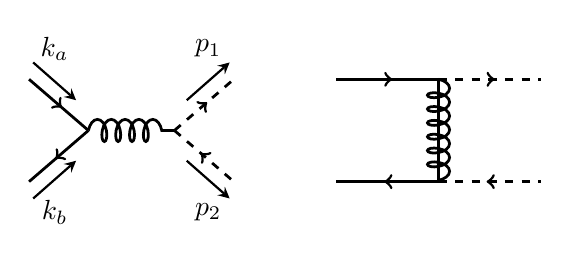
\begin{tikzpicture}[line width=1.0 pt, scale=1.3, arrow/.style={thick,->,shorten >=2pt,shorten <=2pt,>=stealth}]
	\draw[fermion] (-1,0.5)--(-0.42,0);
	\draw[fermionbar] (-1,-0.5)--(-0.42,0);
	\draw[gluon] (-0.42,0)--(0.42,0); 
	\draw[scalar] (0.42,0)--(1,0.5);
	\draw[scalarbar] (0.42,0)--(1,-0.5);
	\draw[arrow] (-1,0.7)--(-0.5,0.26);
	\node at (-0.75,0.8) {$k_a$};
	\draw[arrow] (-1,-0.7)--(-0.5,-0.26);
	\node at (-0.75,-0.8) {$k_b$};
	\draw[arrow] (0.5,0.26)--(1,0.7);
	\node at (0.75,0.8) {$p_1$};
	\draw[arrow] (0.5,-0.26)--(1,-0.7);
	\node at (0.75,-0.8) {$p_2$};
\begin{scope}[shift={(3,0)}]
	\draw[fermion] (-1,0.5)--(0,0.5);
	\draw[fermionbar] (-1,-0.5)--(0,-0.5);
	\draw[fermionnoarrow] (0,0.5)--(0,-0.5);
	\draw[gluon] (0,0.5)--(0,-0.5); 
	\draw[scalar] (0,0.5)--(1,0.5);
	\draw[scalarbar] (0,-0.5)--(1,-0.5);
\end{scope}
\end{tikzpicture}
%\caption{Tree level diagrams for $q\overline{q} \to \tilde{q}\tilde{q}^\dagger$}
\end{center}
%\end{figure}
%\begin{figure}[!htbp]
\begin{center}
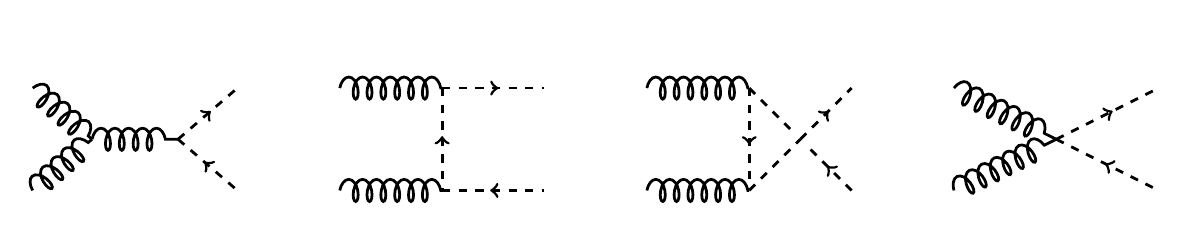
\begin{tikzpicture}[line width=1.0 pt, scale=1.3]
    \node at (0,0) {};
\begin{scope}[shift={(0,-1)}]
	\draw[gluon] (-1,0.5)--(-0.42,0);
	\draw[gluon] (-1,-0.5)--(-0.42,0);
	\draw[gluon] (-0.42,0)--(0.42,0); 
	\draw[scalar] (0.42,0)--(1,0.5);
	\draw[scalarbar] (0.42,0)--(1,-0.5);
\begin{scope}[shift={(3,0)}]
	\draw[gluon] (-1,0.5)--(0,0.5);
	\draw[gluon] (-1,-0.5)--(0,-0.5);
	\draw[scalarbar] (0,0.5)--(0,-0.5);
	\draw[scalar] (0,0.5)--(1,0.5);
	\draw[scalarbar] (0,-0.5)--(1,-0.5);
\end{scope}
\begin{scope}[shift={(6,0)}]
	\draw[gluon] (-1,0.5)--(0,0.5);
	\draw[gluon] (-1,-0.5)--(0,-0.5);
	\draw[scalar] (0,0.5)--(0,-0.5);
	\draw[scalarnoarrow] (0,0.5)--(0.4,0.1);
	\draw[scalarbar] (0.6,-0.1)--(1,-0.5);
	\draw[scalarnoarrow] (0,-0.5)--(0.5,0);
	\draw[scalar] (0.5,0)--(1,0.5);
\end{scope}
\begin{scope}[shift={(9,0)}]
	\draw[gluon] (-1,0.5)--(0,0);
	\draw[gluon] (-1,-0.5)--(0,0);
	\draw[scalarbar] (0,0)--(1,-0.5);
	\draw[scalar] (0,0)--(1,0.5);
\end{scope}
\end{scope}
\end{tikzpicture}
%\caption{Tree level diagrams for $GG \to \tilde{q}\tilde{q}^\dagger$}
\end{center}
%\end{figure}
%\begin{figure}[!htbp]
\begin{center}
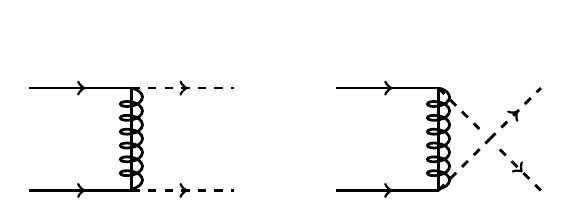
\begin{tikzpicture}[line width=1.0 pt, scale=1.3]
    \node at (0,0) {};
\begin{scope}[shift={(0,-1)}]
	\draw[fermion] (-1,0.5)--(0,0.5);
	\draw[fermion] (-1,-0.5)--(0,-0.5);
	\draw[gluon] (0,0.5)--(0,-0.5);
	\draw[fermionnoarrow] (0,0.5)--(0,-0.5);
	\draw[scalar] (0,0.5)--(1,0.5);
	\draw[scalar] (0,-0.5)--(1,-0.5);;
\begin{scope}[shift={(3,0)}]
	\draw[fermion] (-1,0.5)--(0,0.5);
	\draw[fermion] (-1,-0.5)--(0,-0.5);
	\draw[gluon] (0,0.5)--(0,-0.5);
	\draw[fermionnoarrow] (0,0.5)--(0,-0.5);
	\draw[scalarnoarrow] (0,0.5)--(0.4,0.1);
	\draw[scalar] (0.6,-0.1)--(1,-0.5);
	\draw[scalarnoarrow] (0,-0.5)--(0.5,0);
	\draw[scalar] (0.5,0)--(1,0.5);
\end{scope}
\end{scope}
\end{tikzpicture}
%\caption{Tree level diagrams for $qq \to \tilde{q}\tilde{q}$}
\end{center}
%\end{figure}
%\begin{figure}[!htbp]
\begin{center}
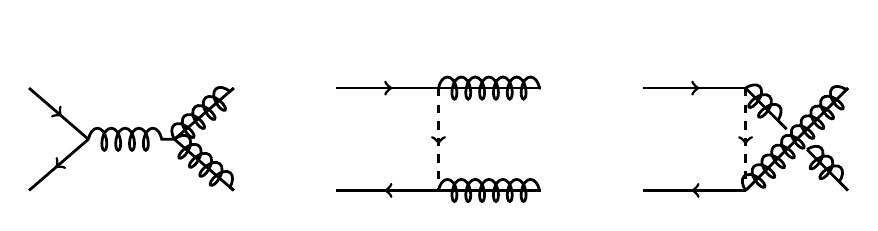
\begin{tikzpicture}[line width=1.0 pt, scale=1.3]
    \node at (0,0) {};
\begin{scope}[shift={(0,-1)}]
	\draw[fermion] (-1,0.5)--(-0.42,0);
	\draw[fermionbar] (-1,-0.5)--(-0.42,0);
	\draw[gluon] (-0.42,0)--(0.42,0); 
	\draw[gluon] (0.42,0)--(1,0.5);
	\draw[fermionnoarrow] (0.42,0)--(1,0.5);
	\draw[gluon] (0.42,0)--(1,-0.5);
	\draw[fermionnoarrow] (0.42,0)--(1,-0.5);
\begin{scope}[shift={(3,0)}]
	\draw[fermion] (-1,0.5)--(0,0.5);
	\draw[fermionbar] (-1,-0.5)--(0,-0.5);
	\draw[scalar] (0,0.5)--(0,-0.5);
	\draw[gluon] (0,0.5)--(1,0.5);
	\draw[fermionnoarrow] (0,0.5)--(1,0.5);
	\draw[gluon] (0,-0.5)--(1,-0.5);
	\draw[fermionnoarrow] (0,-0.5)--(1,-0.5);
\end{scope}
\begin{scope}[shift={(6,0)}]
	\draw[fermion] (-1,0.5)--(0,0.5);
	\draw[fermionbar] (-1,-0.5)--(0,-0.5);
	\draw[scalar] (0,0.5)--(0,-0.5);
	\draw[gluon] (0,0.5)--(0.4,0.1);
	\draw[fermionnoarrow] (0,0.5)--(0.4,0.1);
	\draw[gluon] (0.6,-0.1)--(1,-0.5);
	\draw[fermionnoarrow] (0.6,-0.1)--(1,-0.5);
	\draw[gluon] (0,-0.5)--(1,0.5);
	\draw[fermionnoarrow] (0,-0.5)--(1,0.5);
\end{scope}
\end{scope}
\end{tikzpicture}
%\caption{Tree level diagrams for $q\overline{q} \to \tilde{g}\overline{\tilde{g}}$}
\end{center}
%\end{figure}
%\begin{figure}[!htbp]
\begin{center}
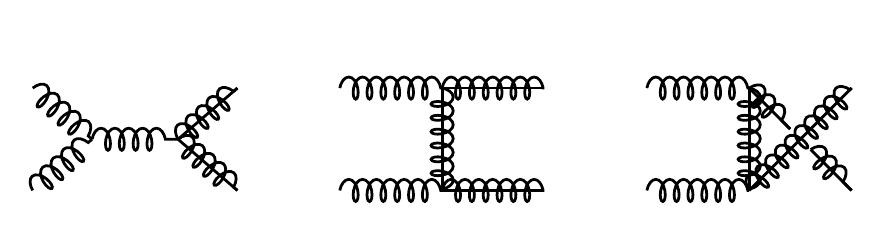
\begin{tikzpicture}[line width=1.0 pt, scale=1.3]
    \node at (0,0) {};
\begin{scope}[shift={(0,-1)}]
	\draw[gluon] (-1,0.5)--(-0.42,0);
	\draw[gluon] (-1,-0.5)--(-0.42,0);
	\draw[gluon] (-0.42,0)--(0.42,0); 
	\draw[gluon] (0.42,0)--(1,0.5);
	\draw[fermionnoarrow] (0.42,0)--(1,0.5);
	\draw[gluon] (0.42,0)--(1,-0.5);
	\draw[fermionnoarrow] (0.42,0)--(1,-0.5);
\begin{scope}[shift={(3,0)}]
	\draw[gluon] (-1,0.5)--(0,0.5);
	\draw[gluon] (-1,-0.5)--(0,-0.5);
	\draw[gluon] (0,0.5)--(0,-0.5);	
	\draw[fermionnoarrow] (0,0.5)--(0,-0.5);
	\draw[gluon] (0,0.5)--(1,0.5);
	\draw[fermionnoarrow] (0,0.5)--(1,0.5);
	\draw[gluon] (0,-0.5)--(1,-0.5);
	\draw[fermionnoarrow] (0,-0.5)--(1,-0.5);
\end{scope}
\begin{scope}[shift={(6,0)}]
	\draw[gluon] (-1,0.5)--(0,0.5);
	\draw[gluon] (-1,-0.5)--(0,-0.5);
	\draw[gluon] (0,0.5)--(0,-0.5);
	\draw[fermionnoarrow] (0,0.5)--(0,-0.5);
	\draw[gluon] (0,0.5)--(0.4,0.1);
	\draw[fermionnoarrow] (0,0.5)--(0.4,0.1);
	\draw[gluon] (0.6,-0.1)--(1,-0.5);
	\draw[fermionnoarrow] (0.6,-0.1)--(1,-0.5);
	\draw[gluon] (0,-0.5)--(1,0.5);
	\draw[fermionnoarrow] (0,-0.5)--(1,0.5);
\end{scope}
\end{scope}
\end{tikzpicture}
%\caption{Tree level diagrams for $GG \to \tilde{g}\overline{\tilde{g}}$}
\end{center}
%\end{figure}
%\begin{figure}[!htbp]
\begin{center}
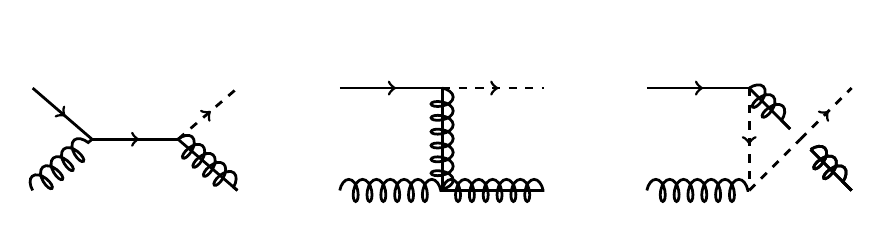
\begin{tikzpicture}[line width=1.0 pt, scale=1.3]
    \node at (0,0) {};
\begin{scope}[shift={(0,-1)}]
	\draw[fermion] (-1,0.5)--(-0.42,0);
	\draw[gluon] (-1,-0.5)--(-0.42,0);
	\draw[fermion] (-0.42,0)--(0.42,0); 
	\draw[scalar] (0.42,0)--(1,0.5);
	\draw[gluon] (0.42,0)--(1,-0.5);
	\draw[fermionnoarrow] (0.42,0)--(1,-0.5);
\begin{scope}[shift={(3,0)}]
	\draw[fermion] (-1,0.5)--(0,0.5);
	\draw[gluon] (-1,-0.5)--(0,-0.5);
	\draw[gluon] (0,0.5)--(0,-0.5);	
	\draw[fermionnoarrow] (0,0.5)--(0,-0.5);
	\draw[scalar] (0,0.5)--(1,0.5);
	\draw[gluon] (0,-0.5)--(1,-0.5);
	\draw[fermionnoarrow] (0,-0.5)--(1,-0.5);
\end{scope}
\begin{scope}[shift={(6,0)}]
	\draw[fermion] (-1,0.5)--(0,0.5);
	\draw[gluon] (-1,-0.5)--(0,-0.5);
	\draw[scalar] (0,0.5)--(0,-0.5);
	\draw[gluon] (0,0.5)--(0.4,0.1);
	\draw[fermionnoarrow] (0,0.5)--(0.4,0.1);
	\draw[gluon] (0.6,-0.1)--(1,-0.5);
	\draw[fermionnoarrow] (0.6,-0.1)--(1,-0.5);
	\draw[gluon] (0.6,-0.1)--(1,-0.5);
	\draw[fermionnoarrow] (0.6,-0.1)--(1,-0.5);
	\draw[scalarnoarrow] (0,-0.5)--(0.5,0);
	\draw[scalar] (0.5,0)--(1,0.5);
\end{scope}
\end{scope}
\end{tikzpicture}
\caption{Tree level diagrams for squark and gluino production at tree level in the MRSSM. The processes $GG \to \tilde{q}\overline{\tilde{q}}$ and $qG \to \tilde{q}\tilde{g}$ are identical to those in the MSSM. The processes $q\overline{q} \to \tilde{q}\overline{\tilde{q}}$ and $qq \to \tilde{q}\tilde{q}$ involve the production of less chiralities than in the MSSM. Also in the $q\tilde{q} \to \tilde{g}\overline{\tilde{g}}$ channel only half of the t-channel squark chiralities occur in the MRSSM. (Anti-)Gluino production via initial gluons $GG \to \tilde{g}\overline{\tilde{g}}$ proceeds via the same diagrams like in the MSSM but its cross section is twice as much in the MRSSM for gluino and antigluino are distinguishable particles.}\label{fig:TreeDiagrams}
\end{center}
\end{figure}
For the calculation the top quark is excluded from the initial state as it is too heavy to be significantly present in hadrons. %Therefore its pdf is approximately zero. 
For consistency reasons also the stop is excluded from the final states. One therefore deals with $n_f-1 = 5$ quark flavors. Using the Feynman rules in the Appendix one obtains the following sums over absolute squared Feynman amplitudes.
\begin{align}
\sum|\mathcal{M}^B|^2(q_i\overline{q}_j \to \tilde{q}\tilde{q}^\dagger) &= \delta_{ij}  \left[ 8 N_c C(F) g_s^4\frac{(n_f-1)}{s^2} + 4 N_c C(F) \hat{g}_s^4\frac{1}{t_{\tilde{g}}^2} - 8 C(F)g_s^2\hat{g}_s^2\frac{1}{ t_{\tilde{g}} s} \right] (tu-m_{\tilde{q}}^4)\nonumber\\
 &+ (1-\delta_{ij}) 4 N_c C(F) \hat{g}_s^4\frac{tu-m_{\tilde{q}}^4}{t_{\tilde{g}}^2} \\
\sum|\mathcal{M}^B|^2(GG \to \tilde{q}\tilde{q}^\dagger) &= 4 (n_f-1) g_s^4 \left[ 2N_c^2C(F) \left(1 - 2\frac{t_{\tilde{q}}u_{\tilde{q}}}{s^2} \right)- 2C(F) \right]\nonumber\\
& \left[ 1 - \epsilon - 2\frac{s m_{\tilde{q}}^2}{t_{\tilde{q}}u_{\tilde{q}}} \left( 1-\frac{s m_{\tilde{q}}^2}{t_{\tilde{q}}u_{\tilde{q}}} \right)\right]\\
\sum|\mathcal{M}^B|^2(q_i q_j \to \tilde{q}\tilde{q}) &= \delta_{ij} 2\hat{g}_s^4 N_c C(F)\left[ \frac{1}{t_{\tilde{g}}^2} + \frac{1}{u_{\tilde{g}}^2} \right] (tu-m_{\tilde{q}}^4)\nonumber\\ 
& + (1-\delta_{ij}) 4 \hat{g}_s^4 N_c C(F) \frac{tu-m_{\tilde{q}}^4}{t_{\tilde{g}}^2}\\
\sum|\mathcal{M}^B|^2(q\overline{q} \to \tilde{g}\overline{\tilde{g}}) &=  8 N_c^2 C(F) g_s^4 \left[ \frac{2m_{\tilde{g}}^2 s + t_{\tilde{g}}^2 + u_{\tilde{g}}^2}{s^2} -\epsilon \right]\nonumber\\
& + 4 N_c^2 C(F) g_s^2 \hat{g}_s^2 \left[ \frac{m_{\tilde{g}}^2 s + t_{\tilde{g}}^2}{s t_{\tilde{q}}} + \frac{m_{\tilde{g}}^2 s + u_{\tilde{g}}^2}{su_{\tilde{q}}} + \epsilon\left( \frac{t_{\tilde{g}}}{t_{\tilde{q}}} + \frac{u_{\tilde{g}}}{u_{\tilde{q}}} \right) \right]\nonumber\\
& + 2C(F)(N_c^2-1) \hat{g}^4_s \left( \frac{t_{\tilde{g}}^2}{t_{\tilde{q}}^2} + \frac{u_{\tilde{g}}^2}{u_{\tilde{q}}^2} \right)\\
%& + 2 \hat{g}_s^4\left[ 2 N_c^2 C(F) \left( \frac{t_{\tilde{g}}^2}{t_{\tilde{q}}^2} + \frac{u_{\tilde{g}}^2}{u_{\tilde{q}}^2} \right) + 2 C(F) \left( 2\frac{m_{\tilde{g}}^2 s}{t_{\tilde{q}}u_{\tilde{q}}} - \frac{t_{\tilde{g}}^2}{t_{\tilde{q}}^2} - \frac{u_{\tilde{g}}^2}{u_{\tilde{q}}^2} \right) \right]\\
\sum|\mathcal{M}^B|^2(GG \to \tilde{g}\overline{\tilde{g}}) &=  16 N_c^3 C(F) g_s^4 \left( 1- \frac{t_{\tilde{g}}u_{\tilde{g}}}{s^2} \right)\nonumber\\
&\left[ \frac{s^2}{t_{\tilde{g}}u_{\tilde{g}}}(1-\epsilon)^2-2(1-\epsilon) + 4\frac{m_{\tilde{g}}^2 s}{t_{\tilde{g}}u_{\tilde{g}}}\left(1-\frac{m_{\tilde{g}}^2 s}{t_{\tilde{g}}u_{\tilde{g}}}  \right) \right]\\
\sum|\mathcal{M}^B|^2(qg \to \tilde{q}\tilde{g}) &=  2g_s^2\hat{g}_s^2 \left[ 2 N_c^2 C(F) \left(1-2\frac{s u_{\tilde{q}}}{t_{\tilde{g}}^2}\right) - 2C(F) \right] \nonumber\\
&\left[ (-1+\epsilon)\frac{t_{\tilde{g}}}{s} + \frac{2(m_{\tilde{g}}^2-m_{\tilde{q}}^2)t_{\tilde{g}}}{s u_{\tilde{q}}}\left( 1+\frac{m_{\tilde{q}}^2}{u_{\tilde{q}}} + \frac{m_{\tilde{g}}^2}{t_{\tilde{g}}} \right) \right]
\end{align}
In view of the renormalization to be performed at the 1-loop level the results are given in $D = 4 - 2\epsilon$ dimensions and it has been distinguished between the gauge coupling $g_s$ from the gluon-quark-quark vertex and its supersymmetric analogue $\hat{g}_s$ from the gluino-squark-quark vertex. The usual Mandelstam variables $s,t,u$ and the following modifications of them are used\footnote{The kinematics of the process is like denoted in fig. \ref{fig:TreeDiagrams}.}
\begin{align}
& s = (k_a + k_b)^2 = (p_1 + p_2)^2\nonumber\\
& t = (k_a - p_1)^2 = (k_b - p_2)^2\nonumber\\
& u = (k_a - p_2)^2 = (k_a - p_2)^2\nonumber\\
& t_{\tilde{g}} = t - m_{\tilde{g}}^2 && t_{\tilde{q}} = t- m_{\tilde{q}}^2\nonumber\\
& u_{\tilde{g}} = u - m_{\tilde{g}}^2 && u_{\tilde{q}} = u- m_{\tilde{q}}^2
\end{align}



\subsection{Partonic Cross Sections}
Having calculated the absolute squared Feynman amplitudes one obtains the partonic cross sections (see Appendix \ref{sec:cross_section}) via
\begin{align}
\frac{\mbox{d}^2 \sigma^B}{\mbox{d}t\ \mbox{d}u} =& \frac{K_{ab}}{s^2} \frac{\pi S_{\epsilon}}{\Gamma(1-\epsilon)} \left[ \frac{tu-m_1^2m_2^2}{\mu^2 s}\right]^{-\epsilon} \Theta(tu-m_1^2m_2^2)\nonumber\\
&\ \Theta(s-4m^2) \delta(s+t+u-m_1^2-m_2^2) \sum |\mathcal{M}^B|^2\label{eq:sigma_tree}
\end{align}
The leading order cross sections are
\begin{align}
\sigma^B(q_i \overline{q}_j \to \tilde{q}\tilde{q}^\dagger) &= \delta_{ij}  \frac{g_s^4}{16\pi s} (n_f-1) \left[ \frac{4}{27} - \frac{16 m_{\tilde{q}}^2}{27s} \right]\nonumber\\
&+ \delta_{ij} \frac{g_s^2\hat{g}_s^2}{16\pi s}  \left[ \left( \frac{4}{27} + \frac{8 m_-^2}{27 s} \right)\beta_{\tilde{q}}  + \left( \frac{8m_{\tilde{g}}^2}{27s} + \frac{8m_-^4}{27s^2} \right)L_1 \right]\nonumber\\
& + \frac{\hat{g}_s^4}{16\pi s} \left[ -\frac{8}{9}\beta_{\tilde{q}} + \left( -\frac{4}{9} - \frac{8m_-^2}{9s} \right)L_1 \right]\\
\sigma^B(GG \to \tilde{q}\tilde{q}^\dagger) &= \frac{(n_f-1) g_s^4}{16\pi s} \left[ \left(\frac{5}{24} + \frac{31 m_{\tilde{q}}^2}{12s}\right)\beta_{\tilde{q}} + \left( \frac{4m_{\tilde{q}}^2}{3s} + \frac{m_{\tilde{q}}^4}{3s^2} \right) \ln \frac{1-\beta_{\tilde{q}}}{1+\beta_{\tilde{q}}} \right]\\
\sigma^B(q_i q_j \to \tilde{q}\tilde{q}) &= \frac{\hat{g}_s^4}{16\pi s} \left[ -\frac{8}{9}\beta_{\tilde{q}} +  \left( -\frac{4}{9} - \frac{8m_-^2}{9s} \right)L_1 \right]\\
\sigma^B(q \overline{q} \to \tilde{g}\overline{\tilde{g}}) &= \frac{g_s^4}{16\pi s} \left[ \frac{16}{9} + \frac{32m_{\tilde{g}}^2}{9s} \right] \beta_{\tilde{g}}\nonumber\\
& + \frac{\hat{g}_s^2 g_s^2}{16\pi s}  \left[ \left( -\frac{4}{3}-\frac{8m_-^2}{3s} \right)\beta_{\tilde{g}} + \left( \frac{8 m_{\tilde{g}}^2}{3s} + \frac{8m_-^4}{3s^2} \right) L_2 \right]\nonumber\\
& + \frac{\hat{g}_s^4}{16\pi s} \left[ \left( \frac{32}{27} + \frac{32 m_-^4}{27(m_-^4 + m_{\tilde{q}}^2s)} \right)\beta_{\tilde{g}} - \frac{64m_-^2}{27s}L_2 \right]\label{eq:qqbar_to_sgsgbar}\\
\sigma^B(GG \to \tilde{g}\overline{\tilde{g}}) &= \frac{g_s^4}{16\pi s} \left[ \left( -6 - \frac{51 m_{\tilde{g}}^2}{2s} \right)\beta_{\tilde{g}} + \left( -\frac{9}{2} - \frac{18 m_{\tilde{g}}^2}{s} + \frac{18 m_{\tilde{g}}^4}{s^2} \right)\ln \frac{1-\beta_{\tilde{g}}}{1+\beta_{\tilde{g}}} \right]\\
\sigma^B(q G \to \tilde{q} \tilde{g}) &= \frac{g_s^2\hat{g}_s^2}{16\pi s} \left[ \frac{\kappa}{s}\left( -\frac{7}{9} - \frac{32 m_{-}^2}{9s} \right) + \left( -\frac{8m_-^2}{9s} + \frac{2m_{\tilde{q}}^2m_-^2}{s^2} + \frac{8 m_-^4}{9s^2} \right)L_3\right.\nonumber\\
&+\left. \left( -1-\frac{2m_-^2}{s} + \frac{2m_{\tilde{q}}m_-^2}{s^2} \right)L_4 \right]
\end{align}
where the abbreviations \cite{Beenakker:1996ch} 
\begin{align}
&\beta_{\tilde{q}} = \sqrt{1-\frac{4 m_{\tilde{q}}^2}{s}} && \beta_{\tilde{g}} = \sqrt{1-\frac{4 m_{\tilde{g}}^2}{s}}\nonumber\\
&m_-^2 = m_{\tilde{g}}^2 - m_{\tilde{q}}^2 && \kappa = \sqrt{(s-m_{\tilde{g}}^2-m_{\tilde{q}}^2)^2-4m_{\tilde{g}}^2m_{\tilde{q}}^2}\nonumber\\
& L_1 = \ln \frac{s+2m_-^2 - s\beta_{\tilde{q}}}{s+2m_-^2 + s\beta_{\tilde{q}}} && L_2= \ln \frac{s - 2m_-^2 - s\beta_{\tilde{g}}}{s - 2m_-^2 + s\beta_{\tilde{g}}}\nonumber\\
& L_3 = \ln \frac{s - m_-^2 - \kappa}{s - m_-^2 + \kappa} && L_4= \ln \frac{s + m_-^2 - \kappa}{s + m_-^2 + \kappa}
\end{align}
are used. The comparison of the cross sections of the MRSSM with those of the MSSM is postponed until the next subsection where the confinement of quarks and gluons within hadrons is accounted for.



\subsection{Hadronic Cross Section}
factorization (pictorial explanation in factorization paper chapter 1.4 and Dissertori and Seymour, Marx page 24 below)\\
Quarks, anti-quarks and gluons are no free particles but are confined within hadrons. As hadrons consist of a variety of the just mentioned partons which share the hadron's momentum one does not have a definite initial state which is assumed in the previous subsection. Fortunately the hadronic cross section for the production of a final state $X$, e.g. $X = \tilde{q} \tilde{q}$, can be obtained by convolving the partonic cross section with the parton density functions of the initial partons.
\begin{align}
\sigma^B_{\mathrm{Had}}(P_1 P_2 \to X) = \int \mbox{d}x_1 \mbox{d}x_2\ f_{P_1/H_1}(x_1) f_{P_2/H_2}(x_2)\ \sigma^B_{\mathrm{Part}} (P_1 P_2 \to X, s = x_ 1x_2 S).
\end{align}
As the production of the final state $X$ may proceed via various initial partons one has to sum over all possible possibilities arising from the initial hadrons $H_1$ and $H_2$:
\begin{align}
\sigma^B_{\mathrm{Had}}(H_1 H_2 \to X) = \sum_{i,j} \sigma^B_{\mathrm{Had}}(P_1 P_2 \to X).
\end{align}
To get an intuitive idea of this factorization consider the hadrons as extended objects consisting of partons\footnote{The proton is considered as composed of three valence quarks: Two up-quarks and one down-quark. In addition there are gluons and seaquarks, i.e. virtual quark-antiquark pairs.} which are permanently interacting which each other. Now consider two colliding hadrons in their center-of-mass frame. Due to Lorentz contraction the hadrons appear as thin discs and the parton's mutual interactions are time-delayed within this frame. This effectively means that a hadron at the time of collision is virtually frozen.\\
maybe picture of colliding disks\\
This in turn implies that the hadron consists at the time of collision of a definite number of partons which can be thought of as carrying a definite fraction of the hadron's momentum $p_{\mathrm{Part}} = x p_{\mathrm{Had}}$ with $x \in \left(0, 1 \right)$. The parton density function $f_{P/H}(x)$ can therefore be understood as the probability of finding a parton $P$ within the hadron $H$ carrying $x$ of its momentum. See \cite{Brock:1993sz} for how to ascertain parton density functions\\
Fig. ... shows a parton density function set for the proton. One can see that the partons most probable to carry a high fraction of momentum are the valence quarks. For lower values of $x$ gluons constitute the major component of the proton.\\
\begin{figure}[!htpb]
\begin{center}
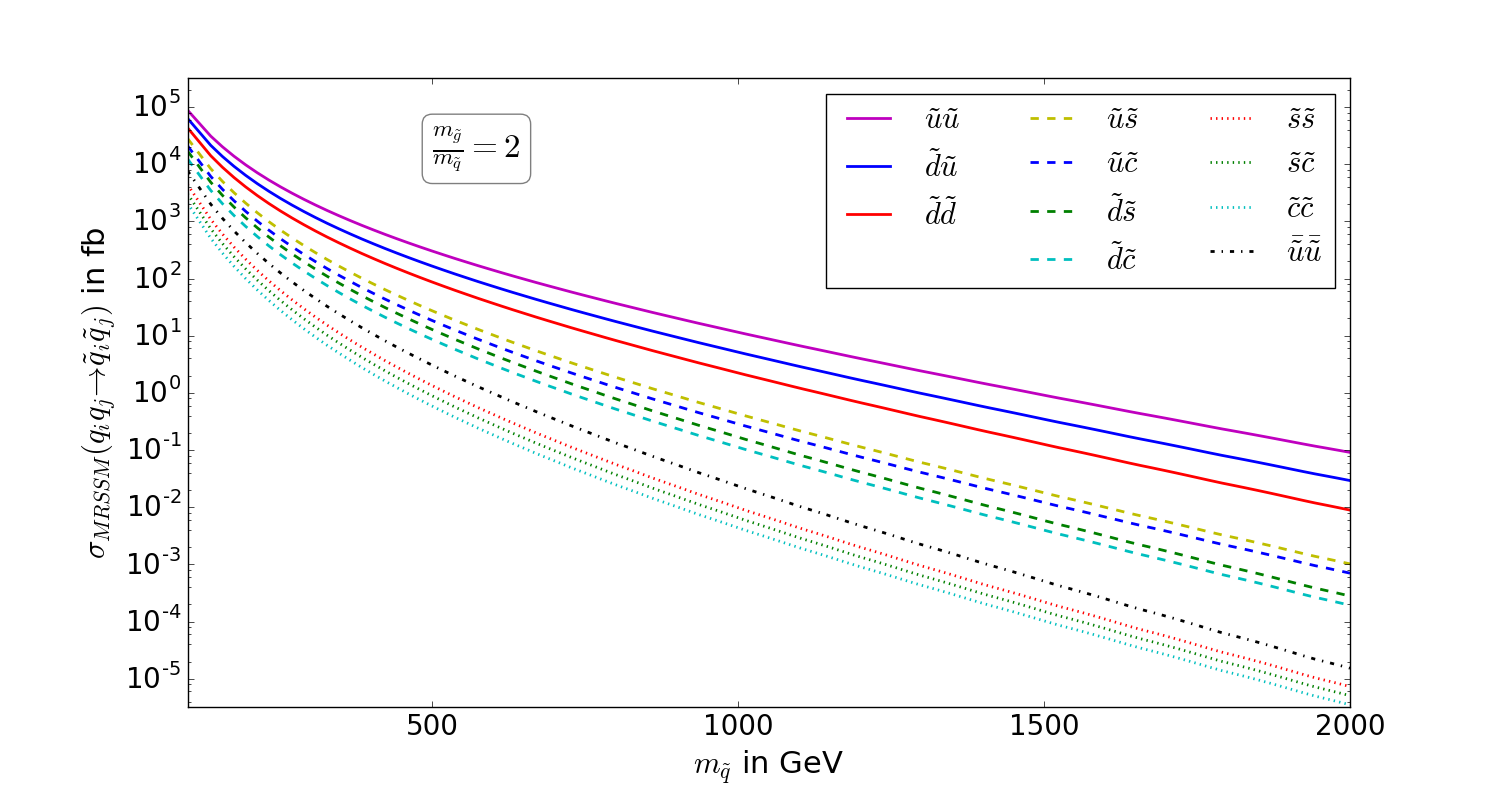
\includegraphics[scale=.45]{figures/MRSSM:q+q->sq+sq_mr=2_seperated}
\caption{Hadronic cross section for squark production in the MRSSM at the LHC at $\sqrt{S} = \unit[13]{GeV}$. The ratio of gluino and squark mass is fixed to 1.5. The parton densities used are $\mathtt{MMHT2014}$ LO with $\alpha_s(M_Z) = 0.135$ in the 5-flavor scheme \cite{Harland-Lang:2014zoa}. As renormalization and factorization scale $\mu_R = \mu_F = \frac{m_1 + m_2}{2}$ has been chosen, where $m_i$ are the final state particle masses.} \label{fig:TreeXsection}
\end{center}
\end{figure}
Fig.\ref{fig:TreeXsection} shows the hadronic cross section for the production of various squarks. These can only be produced by their supersymmetric partner, e.g. two up-squarks can only be produced by two up-quarks. One therefore sees the influence of the parton distribution functions quite nicely: The up-squark production is the dominant contribution to squark production. Apart from the solid lines in fig.\ref{fig:TreeXsection} which correspond to the production of first generation squarks, also the cross section of mixed first and second generation (dashed lines) and second generation squarks is shown. The dashed dotted line shows the cross section of the charged conjugated particles of the dominant channel.\\
refer to Kribs, Martin
\begin{figure}[!htpb]
\begin{center}
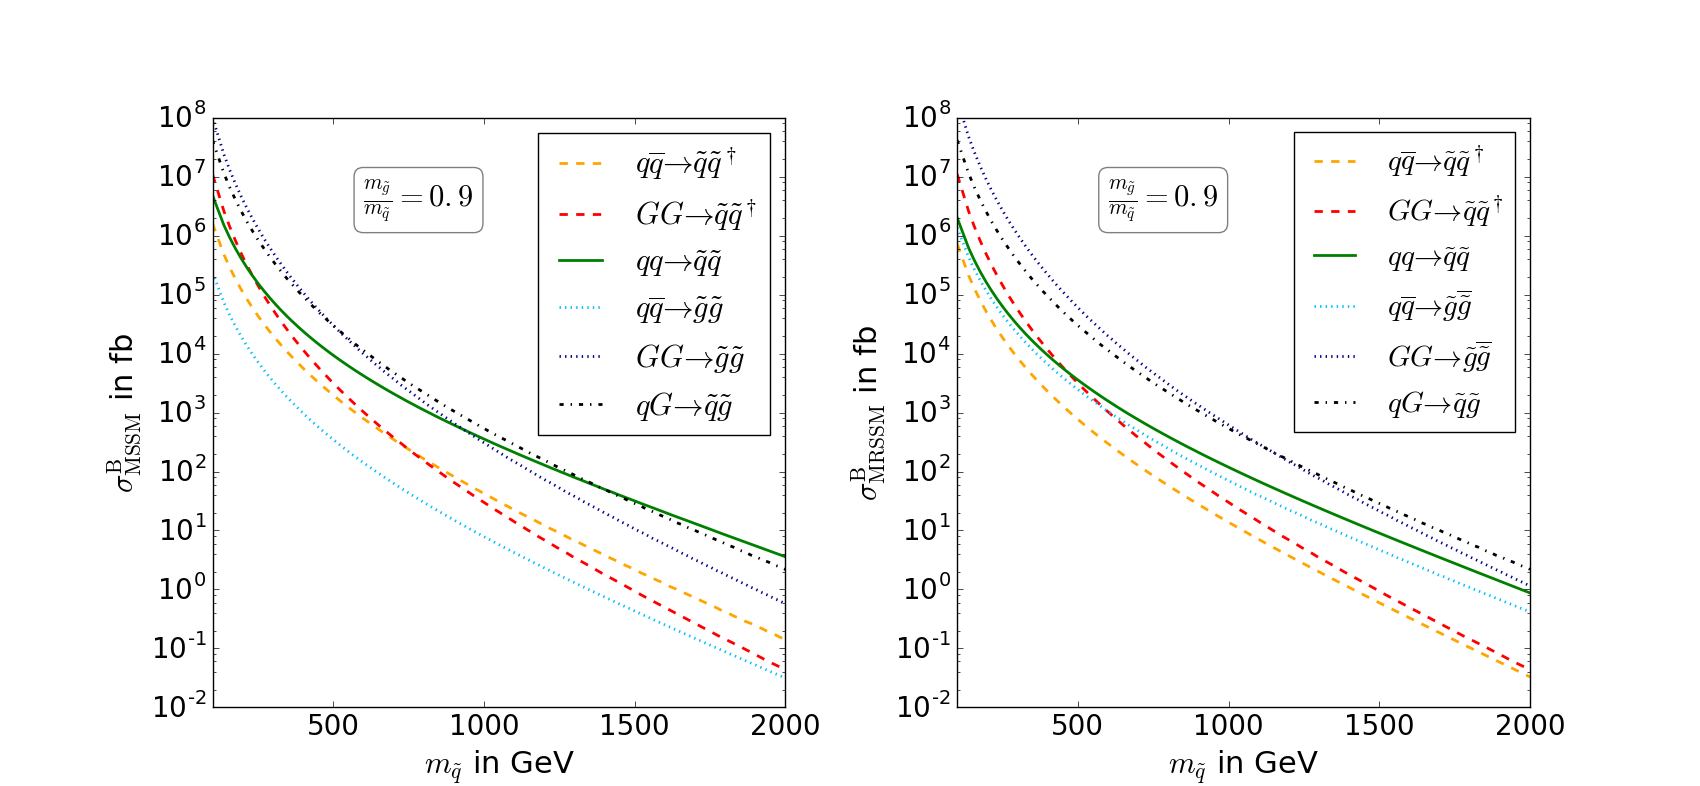
\includegraphics[scale=.4]{figures/mr=0,9_MSSM+MRSSM}
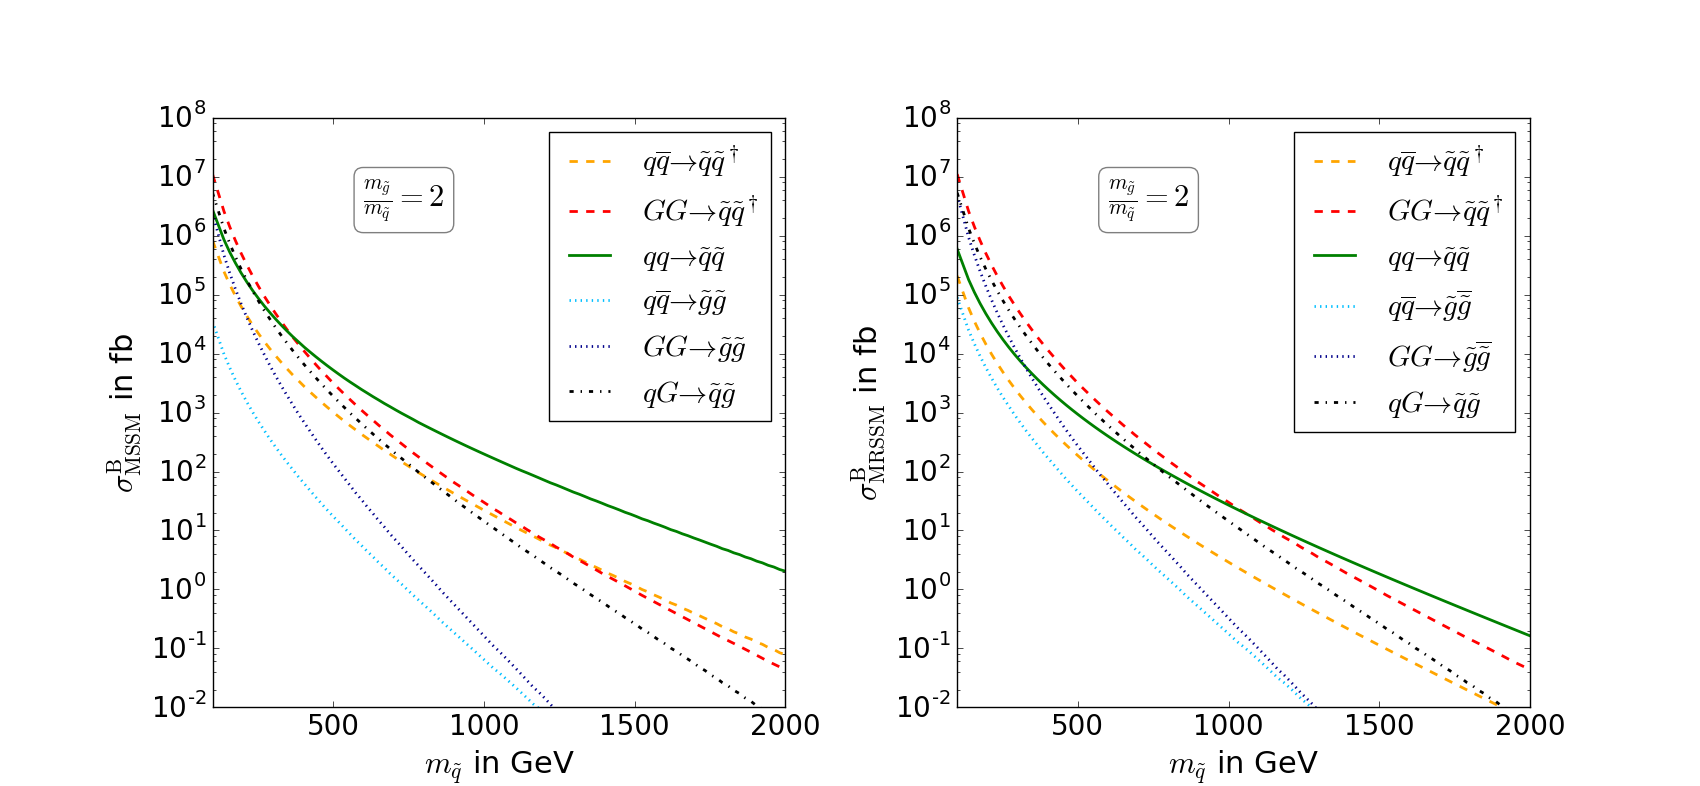
\includegraphics[scale=.4]{figures/mr=2_MSSM+MRSSM}
\caption{Hadronic cross section for squark and gluino production in the MSSM (left-hand side) and MRSSM (right-hand side) at the LHC at $\sqrt{S} = \unit[13]{GeV}$. The ratio of gluino and squark mass is fixed to 0.9 (first row) and 2 (second row). In the final state it has been summed over all squark flavors expect for staus. For the channels $qq \to \tilde{q}\tilde{q}$ and $qG \to \tilde{q}\tilde{G}$ also the charge conjugated process is included. The parton densities used are $\mathtt{MMHT2014}$ LO with $\alpha_s(M_Z) = 0.135$ in the 5-flavor scheme \cite{Harland-Lang:2014zoa}. As renormalization and factorization scale $\mu_R = \mu_F = \frac{m_1 + m_2}{2}$ has been chosen, where $m_i$ are the final state particle masses.} \label{fig:TreeXsection}
\end{center}
\end{figure}


\subsubsection*{The process $q_i \overline{q}_j \to \tilde{q}\tilde{q}^\dagger$}
The production of a squark and an antisquark through a quark and an antiquark in the initial state originates from two types of Feynman diagrams. The first one has an $s$-channel gluon and is the same in the MSSM and in the MRSSM. The second one exhibits a difference due to the $t$-channel gluino which is no Majorana particle in the MRSSM. 
\begin{figure}[!htbp]
\begin{center}
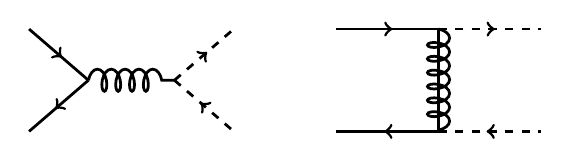
\begin{tikzpicture}[line width=1.0 pt, scale=1.3]
	\draw[fermion] (-1,0.5)--(-0.42,0);
	\draw[fermionbar] (-1,-0.5)--(-0.42,0);
	\draw[gluon] (-0.42,0)--(0.42,0); 
	\draw[scalar] (0.42,0)--(1,0.5);
	\draw[scalarbar] (0.42,0)--(1,-0.5);
\begin{scope}[shift={(3,0)}]
	\draw[fermion] (-1,0.5)--(0,0.5);
	\draw[fermionbar] (-1,-0.5)--(0,-0.5);
	\draw[fermionnoarrow] (0,0.5)--(0,-0.5);
	\draw[gluon] (0,0.5)--(0,-0.5); 
	\draw[scalar] (0,0.5)--(1,0.5);
	\draw[scalarbar] (0,-0.5)--(1,-0.5);
\end{scope}
\end{tikzpicture}
\caption{Tree level diagrams for $q\overline{q} \to \tilde{q}\tilde{q}^\dagger$}
\end{center}
\end{figure}
To see this one can either just apply the Feynman rules in Appendix \ref{sec:FeynmanRules} or think of the conservation of R-charge: Left handed squarks have R-charge +1 and right handed squarks have R-charge -1. Antiparticles have the opposite R-charge of their corresponding particles. The final state particles have to meet the total R-charge zero from the initial state. Because of this one only has $\tilde{q}_L \overline{\tilde{q}}_L$ and $\tilde{q}_R \overline{\tilde{q}}_R$ as the final states in the MRSSM whereas in the MSSM one actually has four instead of two t-channel diagrams: The corresponding final states are $\tilde{q}_L \overline{\tilde{q}}_L$, $\tilde{q}_R \overline{\tilde{q}}_R$, $\tilde{q}_L \overline{\tilde{q}}_R$ and $\overline{\tilde{q}}_R \tilde{q}_L$. Consequently contributions from the $t$-channel diagrams are suppressed in the MRSSM in comparison to the MSSM. As visible in fig. \ref{fig:TreeXsection} this suppression grows with the masses. The reason for this lies in the gluino mass dependence of the $t$-channel diagrams which is explained in the discussion of squark production.\\
If the initial state quarks are of different flavor the $s$-channel diagram is absent.

\subsubsection*{The process $GG \to \tilde{q}\tilde{q}^\dagger$}
This process has the same cross section in the MRSSM and in the MSSM for also in the MSSM only like chirality squark and antisquark $\tilde{q}_A\tilde{q}_A^\dagger$ with $A \in {L,R}$ can be produced

\subsubsection*{The process $q_i q_j \to \tilde{q}\tilde{q}$}
In the MRSSM only the production of unlike chirality squarks $\tilde{q}_L \tilde{q}_R$ is allowed whilst in the MSSM also like chirality squarks can be produced. This is again a consequence of the conservation of R-charge. The upshot of this is a suppression of squark production in the MRSSM in comparison to the MSSM. To be more explicit the suppression of squark production in the MRSSM grows with the gluino mass. This can be understood as follows: As in the MRSSM a left handed squark needs to be produced with a right handed squark one can read off from the Feynman rules given in Appendix \ref{sec:FeynmanRules} that the gluino propagator $i\frac{\slashed{p}+m_{\tilde{g}}}{p^2-m_{\tilde{g}}^2}$ is sandwiched between the projectors $P_L$ and $P_R$ which leads to the cancellation of the gluino mass in the numerator. Therefore for small momenta of the gluino compared to the gluino mass one gets $\mathcal{M}$ $\sim \frac{1}{m_{\tilde{g}}^2}$ in the MRSSM while in the MSSM one finds a suppression proportional to $\frac{1}{m_{\tilde{g}}}$.\\
When considering squark production one has to sum over all $|\mathcal{M}|^2$ with different helicity. The diagrams for those different final state helicities are shown for flavor like squark production in tab. \ref{tab:squark_likeflavor} and for flavor unlike squark production in tab. \ref{tab:squark_unlikeflavor} for the MSSM and the MRSSM. To avoid double counting one needs to weight $|\mathcal{M}|^2(qq\to \tilde{q}_L\tilde{q}_L)$ and $|\mathcal{M}|^2(qq\to \tilde{q}_R\tilde{q}_R)$ with a statistical factor of $\frac{1}{2}$ as one integrates over all momenta of both particles to arrive at the cross section.\footnote{Alternatively one could discard the $u$-channel (or $t$-channel) diagram and omit the weighting with $\frac{1}{2}$.}
\begin{table}[!htpb]
\begin{center}
\begin{tabular}{c|c}
MSSM & MRSSM \\
\hline
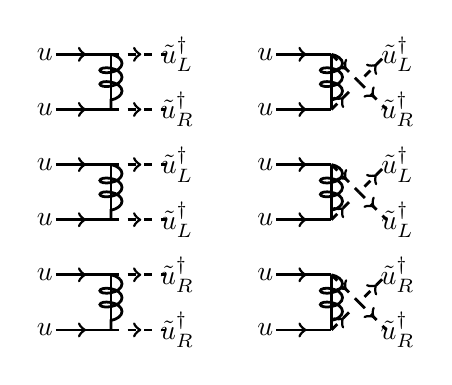
\begin{tikzpicture}[line width=1.0 pt, scale=0.7]
	\draw[fermion] (0,1)--(1,1);
	\draw[fermion] (0,0)--(1,0);
	\draw[fermionnoarrow] (1,1)--(1,0);
	\draw[gluon] (1,1)--(1,0);
	\draw[scalar] (1,1)--(2,1);
	\draw[scalar] (1,0)--(2,0);
	\node at (-0.2,1) {$u$};
	\node at (-0.2,0) {$u$};
	\node at (2.2,1) {$\tilde{u}_L^\dagger$};
	\node at (2.2,0) {$\tilde{u}_R^\dagger$};
\begin{scope}[shift={(4,0)}]
	\draw[fermion] (0,1)--(1,1);
	\draw[fermion] (0,0)--(1,0);
	\draw[fermionnoarrow] (1,1)--(1,0);
	\draw[gluon] (1,1)--(1,0);
	\draw[scalar] (1,1)--(1.5,0.5);
	\draw[scalar] (1.5,0.5)--(2,0);
	\draw[scalar] (1,0)--(1.4,0.4);
	\draw[scalar] (1.6,0.6)--(2,1);
	\node at (-0.2,1) {$u$};
	\node at (-0.2,0) {$u$};
	\node at (2.2,1) {$\tilde{u}_L^\dagger$};
	\node at (2.2,0) {$\tilde{u}_R^\dagger$};
\end{scope}
\begin{scope}[shift={(0,-2)}]
	\draw[fermion] (0,1)--(1,1);
	\draw[fermion] (0,0)--(1,0);
	\draw[fermionnoarrow] (1,1)--(1,0);
	\draw[gluon] (1,1)--(1,0);
	\draw[scalar] (1,1)--(2,1);
	\draw[scalar] (1,0)--(2,0);
	\node at (-0.2,1) {$u$};
	\node at (-0.2,0) {$u$};
	\node at (2.2,1) {$\tilde{u}_L^\dagger$};
	\node at (2.2,0) {$\tilde{u}_L^\dagger$};
\end{scope}
\begin{scope}[shift={(4,-2)}]
	\draw[fermion] (0,1)--(1,1);
	\draw[fermion] (0,0)--(1,0);
	\draw[fermionnoarrow] (1,1)--(1,0);
	\draw[gluon] (1,1)--(1,0);
	\draw[scalar] (1,1)--(1.5,0.5);
	\draw[scalar] (1.5,0.5)--(2,0);
	\draw[scalar] (1,0)--(1.4,0.4);
	\draw[scalar] (1.6,0.6)--(2,1);
	\node at (-0.2,1) {$u$};
	\node at (-0.2,0) {$u$};
	\node at (2.2,1) {$\tilde{u}_L^\dagger$};
	\node at (2.2,0) {$\tilde{u}_L^\dagger$};
\end{scope}
\begin{scope}[shift={(0,-4)}]
	\draw[fermion] (0,1)--(1,1);
	\draw[fermion] (0,0)--(1,0);
	\draw[fermionnoarrow] (1,1)--(1,0);
	\draw[gluon] (1,1)--(1,0);
	\draw[scalar] (1,1)--(2,1);
	\draw[scalar] (1,0)--(2,0);
	\node at (-0.2,1) {$u$};
	\node at (-0.2,0) {$u$};
	\node at (2.2,1) {$\tilde{u}_R^\dagger$};
	\node at (2.2,0) {$\tilde{u}_R^\dagger$};
\end{scope}
\begin{scope}[shift={(4,-4)}]
	\draw[fermion] (0,1)--(1,1);
	\draw[fermion] (0,0)--(1,0);
	\draw[fermionnoarrow] (1,1)--(1,0);
	\draw[gluon] (1,1)--(1,0);
	\draw[scalar] (1,1)--(1.5,0.5);
	\draw[scalar] (1.5,0.5)--(2,0);
	\draw[scalar] (1,0)--(1.4,0.4);
	\draw[scalar] (1.6,0.6)--(2,1);
	\node at (-0.2,1) {$u$};
	\node at (-0.2,0) {$u$};
	\node at (2.2,1) {$\tilde{u}_R^\dagger$};
	\node at (2.2,0) {$\tilde{u}_R^\dagger$};
\end{scope}
\end{tikzpicture} & 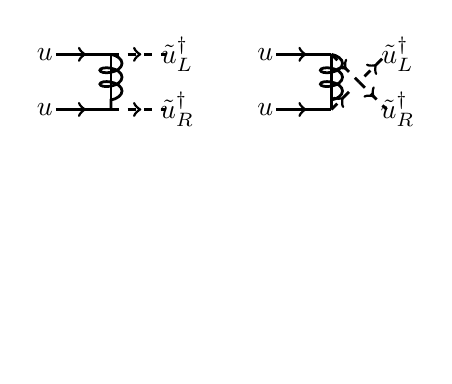
\begin{tikzpicture}[line width=1.0 pt, scale=0.7]
	\draw[fermion] (0,1)--(1,1);
	\draw[fermion] (0,0)--(1,0);
	\draw[fermionnoarrow] (1,1)--(1,0);
	\draw[gluon] (1,1)--(1,0);
	\draw[scalar] (1,1)--(2,1);
	\draw[scalar] (1,0)--(2,0);
	\node at (-0.2,1) {$u$};
	\node at (-0.2,0) {$u$};
	\node at (2.2,1) {$\tilde{u}_L^\dagger$};
	\node at (2.2,0) {$\tilde{u}_R^\dagger$};
\begin{scope}[shift={(4,0)}]
	\draw[fermion] (0,1)--(1,1);
	\draw[fermion] (0,0)--(1,0);
	\draw[fermionnoarrow] (1,1)--(1,0);
	\draw[gluon] (1,1)--(1,0);
	\draw[scalar] (1,1)--(1.5,0.5);
	\draw[scalar] (1.5,0.5)--(2,0);
	\draw[scalar] (1,0)--(1.4,0.4);
	\draw[scalar] (1.6,0.6)--(2,1);
	\node at (-0.2,1) {$u$};
	\node at (-0.2,0) {$u$};
	\node at (2.2,1) {$\tilde{u}_L^\dagger$};
	\node at (2.2,0) {$\tilde{u}_R^\dagger$};
\end{scope}
\begin{scope}[shift={(0,-4.3)}]
\node at (0,0) {};
\end{scope}
\end{tikzpicture} 
\end{tabular}
\caption{All Feynman diagrams contributing to flavor like squark production in the MSSM and the MRSSM for the example of $u$-quarks. For the MSSM the absolute squared Feynman amplitudes from the diagrams with chirality like squarks need to be weighted with a factor of $\frac{1}{2}$.}\label{tab:squark_likeflavor}
\end{center}
\end{table}
\begin{table}[!htpb]
\begin{center}
\begin{tabular}{c|c}
MSSM & MRSSM \\
\hline
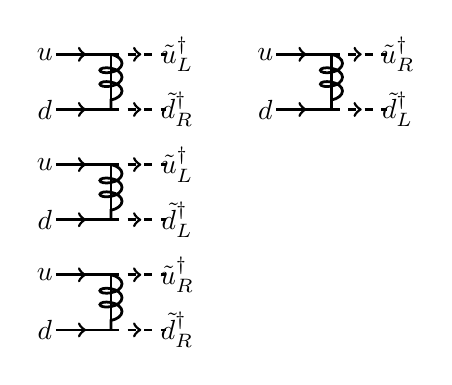
\begin{tikzpicture}[line width=1.0 pt, scale=0.7]
	\draw[fermion] (0,1)--(1,1);
	\draw[fermion] (0,0)--(1,0);
	\draw[fermionnoarrow] (1,1)--(1,0);
	\draw[gluon] (1,1)--(1,0);
	\draw[scalar] (1,1)--(2,1);
	\draw[scalar] (1,0)--(2,0);
	\node at (-0.2,1) {$u$};
	\node at (-0.2,0) {$d$};
	\node at (2.2,1) {$\tilde{u}_L^\dagger$};
	\node at (2.2,0) {$\tilde{d}_R^\dagger$};
\begin{scope}[shift={(4,0)}]
	\draw[fermion] (0,1)--(1,1);
	\draw[fermion] (0,0)--(1,0);
	\draw[fermionnoarrow] (1,1)--(1,0);
	\draw[gluon] (1,1)--(1,0);
	\draw[scalar] (1,1)--(2,1);
	\draw[scalar] (1,0)--(2,0);
	\node at (-0.2,1) {$u$};
	\node at (-0.2,0) {$d$};
	\node at (2.2,1) {$\tilde{u}_R^\dagger$};
	\node at (2.2,0) {$\tilde{d}_L^\dagger$};
\end{scope}
\begin{scope}[shift={(0,-2)}]
	\draw[fermion] (0,1)--(1,1);
	\draw[fermion] (0,0)--(1,0);
	\draw[fermionnoarrow] (1,1)--(1,0);
	\draw[gluon] (1,1)--(1,0);
	\draw[scalar] (1,1)--(2,1);
	\draw[scalar] (1,0)--(2,0);
	\node at (-0.2,1) {$u$};
	\node at (-0.2,0) {$d$};
	\node at (2.2,1) {$\tilde{u}_L^\dagger$};
	\node at (2.2,0) {$\tilde{d}_L^\dagger$};
\end{scope}
\begin{scope}[shift={(0,-4)}]
	\draw[fermion] (0,1)--(1,1);
	\draw[fermion] (0,0)--(1,0);
	\draw[fermionnoarrow] (1,1)--(1,0);
	\draw[gluon] (1,1)--(1,0);
	\draw[scalar] (1,1)--(2,1);
	\draw[scalar] (1,0)--(2,0);
	\node at (-0.2,1) {$u$};
	\node at (-0.2,0) {$d$};
	\node at (2.2,1) {$\tilde{u}_R^\dagger$};
	\node at (2.2,0) {$\tilde{d}_R^\dagger$};
\end{scope}
\end{tikzpicture} & 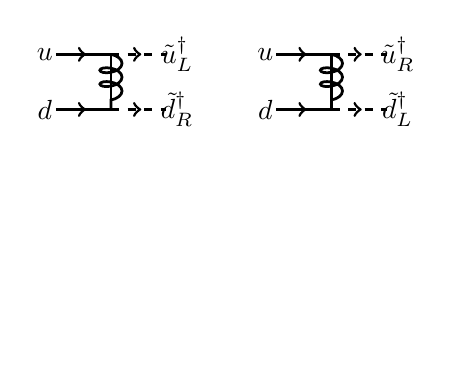
\begin{tikzpicture}[line width=1.0 pt, scale=0.7]
	\draw[fermion] (0,1)--(1,1);
	\draw[fermion] (0,0)--(1,0);
	\draw[fermionnoarrow] (1,1)--(1,0);
	\draw[gluon] (1,1)--(1,0);
	\draw[scalar] (1,1)--(2,1);
	\draw[scalar] (1,0)--(2,0);
	\node at (-0.2,1) {$u$};
	\node at (-0.2,0) {$d$};
	\node at (2.2,1) {$\tilde{u}_L^\dagger$};
	\node at (2.2,0) {$\tilde{d}_R^\dagger$};
\begin{scope}[shift={(4,0)}]
	\draw[fermion] (0,1)--(1,1);
	\draw[fermion] (0,0)--(1,0);
	\draw[fermionnoarrow] (1,1)--(1,0);
	\draw[gluon] (1,1)--(1,0);
	\draw[scalar] (1,1)--(2,1);
	\draw[scalar] (1,0)--(2,0);
	\node at (-0.2,1) {$u$};
	\node at (-0.2,0) {$d$};
	\node at (2.2,1) {$\tilde{u}_R^\dagger$};
	\node at (2.2,0) {$\tilde{d}_L^\dagger$};
\end{scope}
\begin{scope}[shift={(0,-4.3)}]
\node at (0,0) {};
\end{scope}
\end{tikzpicture} 
\end{tabular}
\caption{All Feynman diagrams contributing to flavor unlike squark production in the MSSM and the MRSSM for the example of $u$- and $d$-quarks.}\label{tab:squark_unlikeflavor}
\end{center}
\end{table}\\
Because of the absence of chirality like squarks in the final state in the MRSSM (and a missing interference of the two diagrams in tab. \ref{tab:squark_likeflavor} in the MRSSM) the cross section of flavor like and unlike squarks is the same in the MRSSM, i.e. on the partonic level:\\ $\sigma^{\mathrm{B}}_{\mathrm{Part,\ MRSSM}}(\tilde{u}_L\tilde{u}_R) = \sigma^{\mathrm{B}}_{\mathrm{Part,\ MRSSM}}(\tilde{u}_L\tilde{d}_R)$. That is however not true in the MSSM. 


\subsubsection*{The process $q \overline{q} \to \tilde{g}\overline{\tilde{g}}$}
In contrast to the MSSM no statistical factor of $\frac{1}{2}$ is taken into account when turning from $|\mathcal{M}|^2$ to $\sigma$. This is because gluino and antigluino are distinguishable particles. Still in comparison to the MSSM cross section only the first line in \ref{eq:qqbar_to_sgsgbar} is doubled up as the other two lines origin from an $t$ or $u$ channel squark which occurs in only one instead of two chiralities. Furthermore an interference term from the $t$ or $u$ channel diagram which occurs in the MSSM is absent in the MRSSM.
% this interference term causes a huge difference, that's been checked by Philip via Madgraph

\subsubsection*{The process $GG \to \tilde{g}\overline{\tilde{g}}$}
As in the previous process the MRSSM cross section for $GG \to \tilde{g}\overline{\tilde{g}}$ receives no statistical factor of $\frac{1}{2}$. As there are no further differences between MSSM and MRSSM in this channel, the MRSSM cross section is simply twice as large as in the MSSM.

\subsubsection*{The process $q G \to \tilde{q} \tilde{g}$}
This process is exactly the same in the MSSM and MRSSM.
\\
refer to Vernoica Sanz: How many SUpersymmetries?

\begin{figure}[!htpb]
\begin{center}
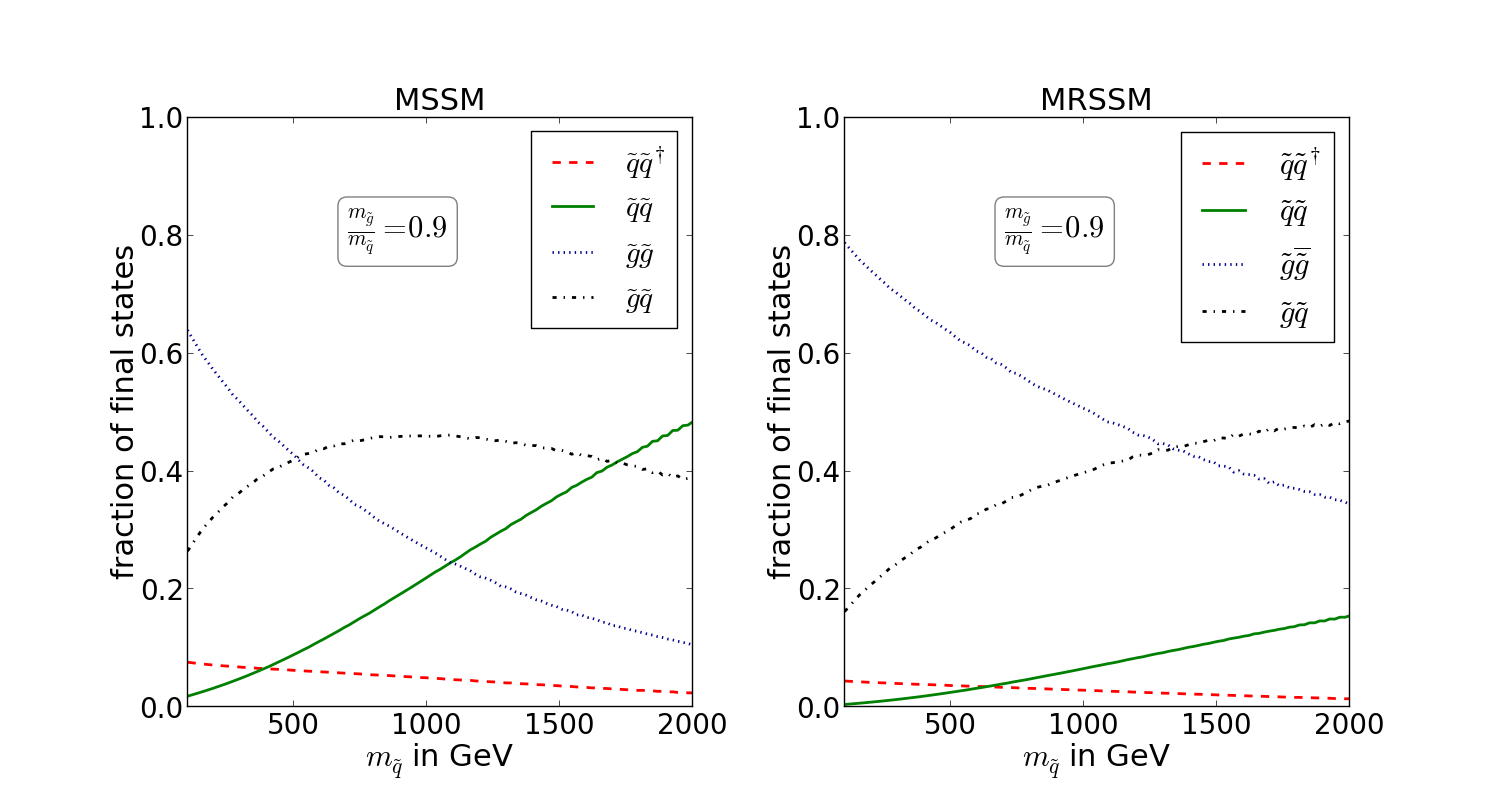
\includegraphics[scale=.45]{figures/rel_weights_mr=0,9_MSSM+MRSSM}
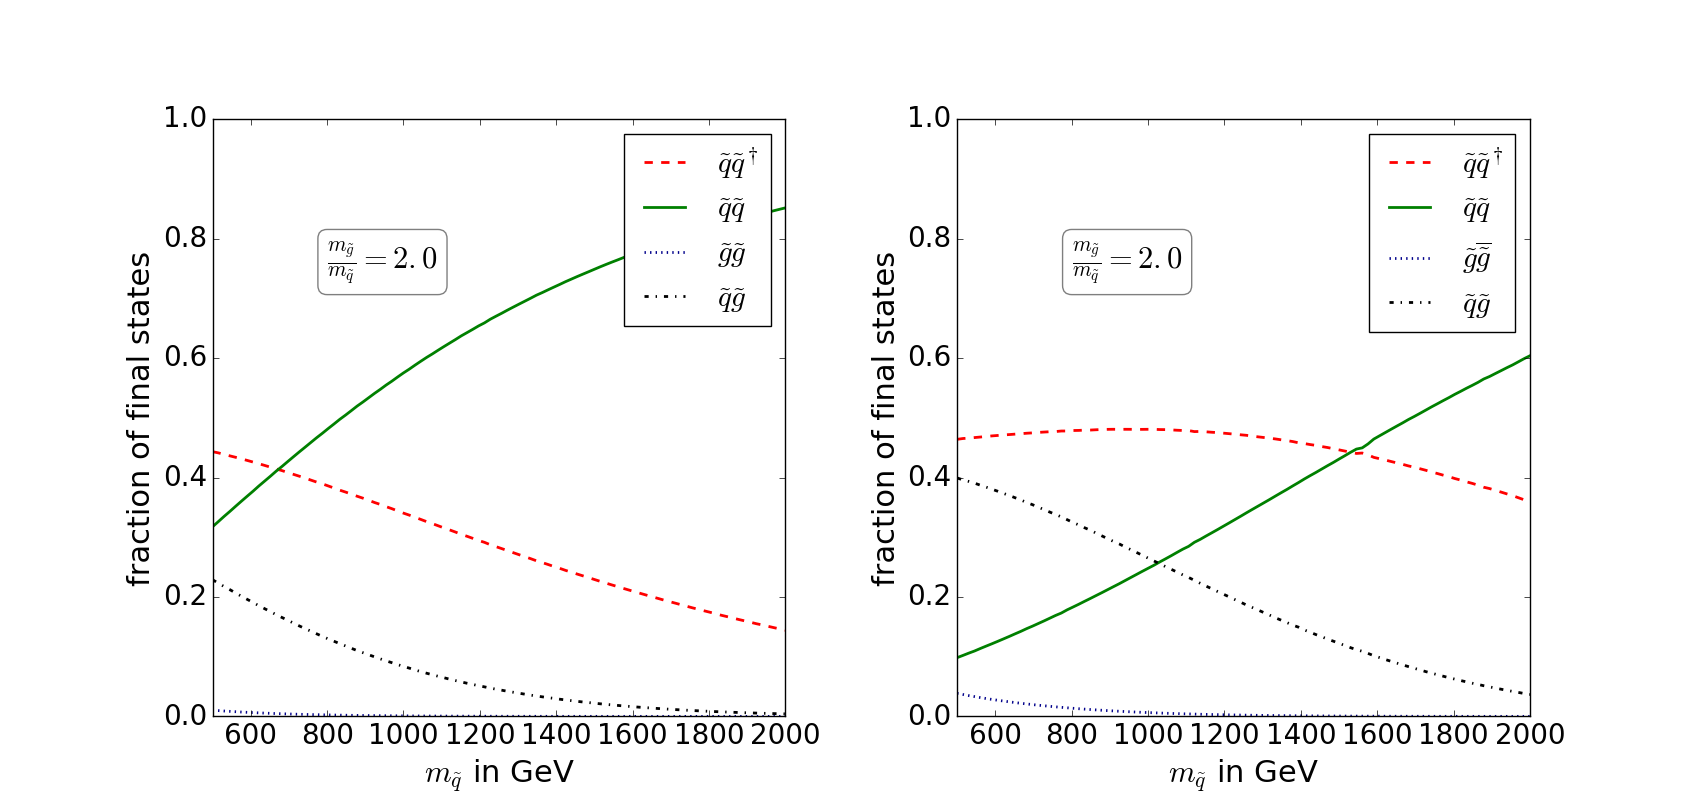
\includegraphics[scale=.45]{figures/rel_weights_mr=2_MSSM+MRSSM}
\caption{Relative contributions of the indicated final states on the total hadronic cross section in the MSSM (left-hand side) and MRSSM (right-hand side) at the LHC at $\sqrt{S} = \unit[13]{GeV}$. The ratio of gluino and squark mass is fixed to 0.9 (first row) and 2 (second row). In the final state it has been summed over all squark flavors expect for staus. For the channels $qq \to \tilde{q}\tilde{q}$ and $qG \to \tilde{q}\tilde{G}$ also the charge conjugated process is included. The parton densities and the renormalization and factorization scale are chosen as in fig. \ref{fig:TreeXsection}.}\label{fig:TreeLevelSigma_0,9_2}
\end{center}
\end{figure}

\begin{figure}[!htpb]
\begin{center}
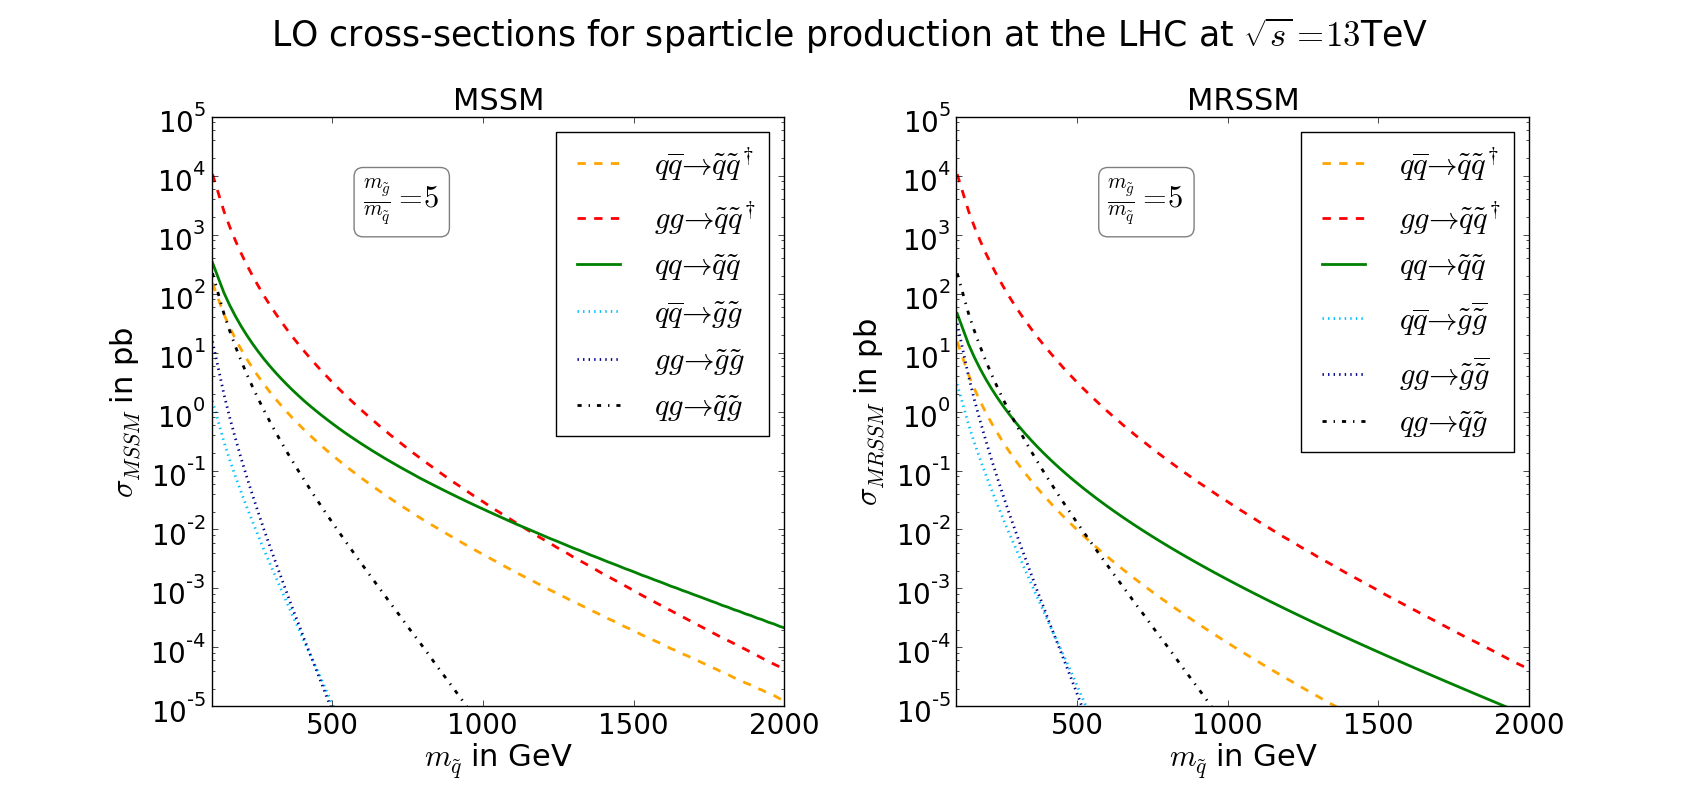
\includegraphics[scale=.4]{figures/mr=5_MSSM+MRSSM}
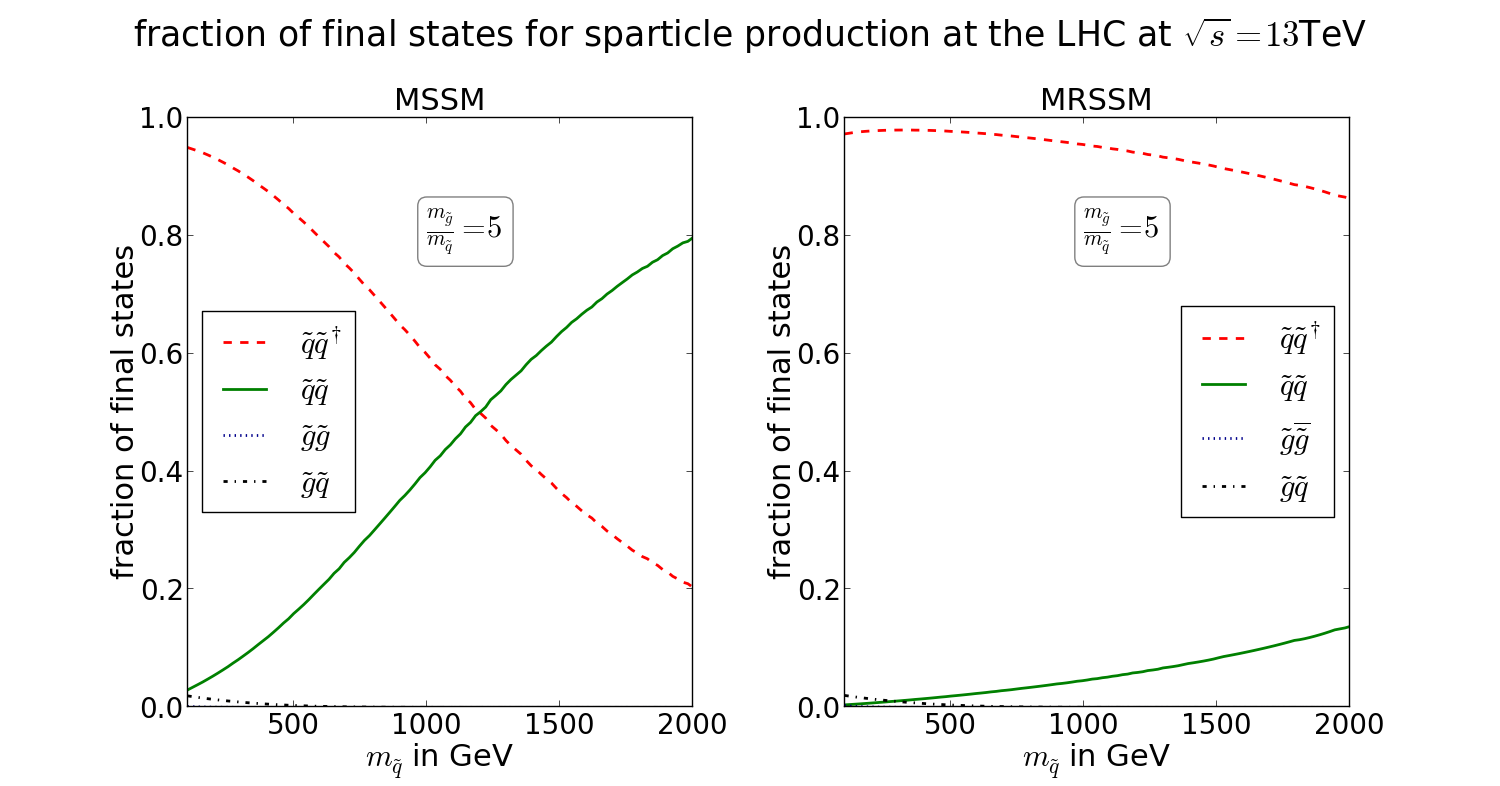
\includegraphics[scale=.45]{figures/rel_weights_mr=5_MSSM+MRSSM}
\caption{Hadronic cross section for squark and gluino production (in the first row) and relative contributions of the indicated final states on the total hadronic cross section in the MSSM (left-hand side) and MRSSM (right-hand side) at the LHC at $\sqrt{S} = \unit[13]{GeV}$. The ratio of gluino and squark mass is fixed to 5. In the final state it has been summed over all squark flavors expect for staus. For the channels $qq \to \tilde{q}\tilde{q}$ and $qG \to \tilde{q}\tilde{G}$ also the charge conjugated process is included. The parton densities and the renormalization and factorization scale are chosen as in fig. \ref{fig:TreeXsection}.}
\end{center}
\end{figure}


\begin{figure}[!htpb]
\begin{center}
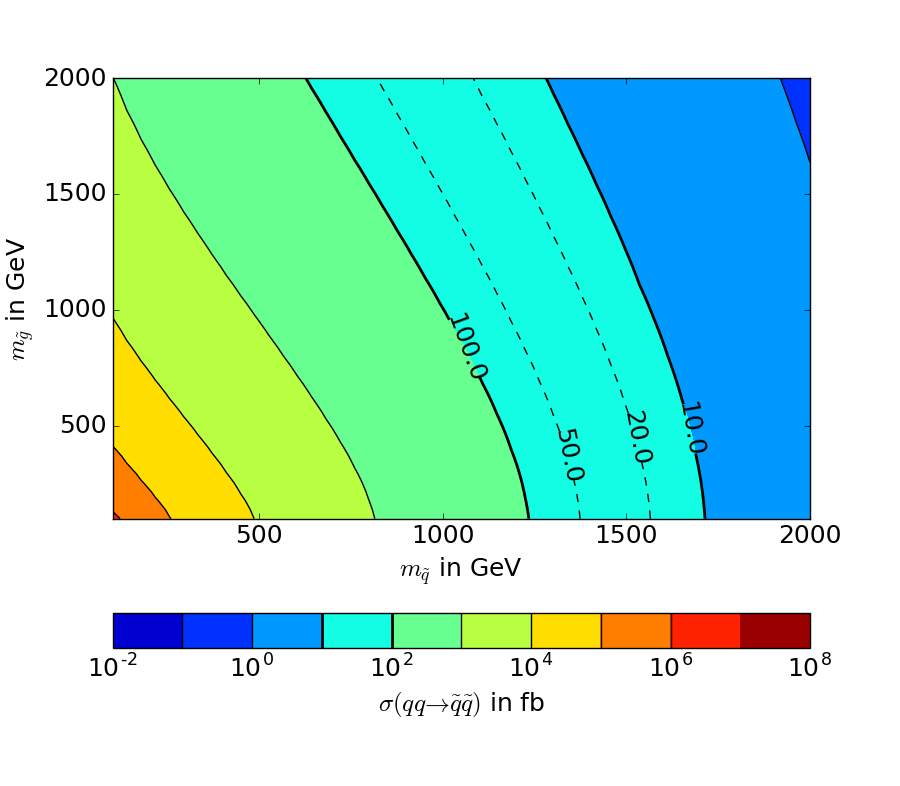
\includegraphics[scale=.6]{figures/contour_MRSSM_squarks}
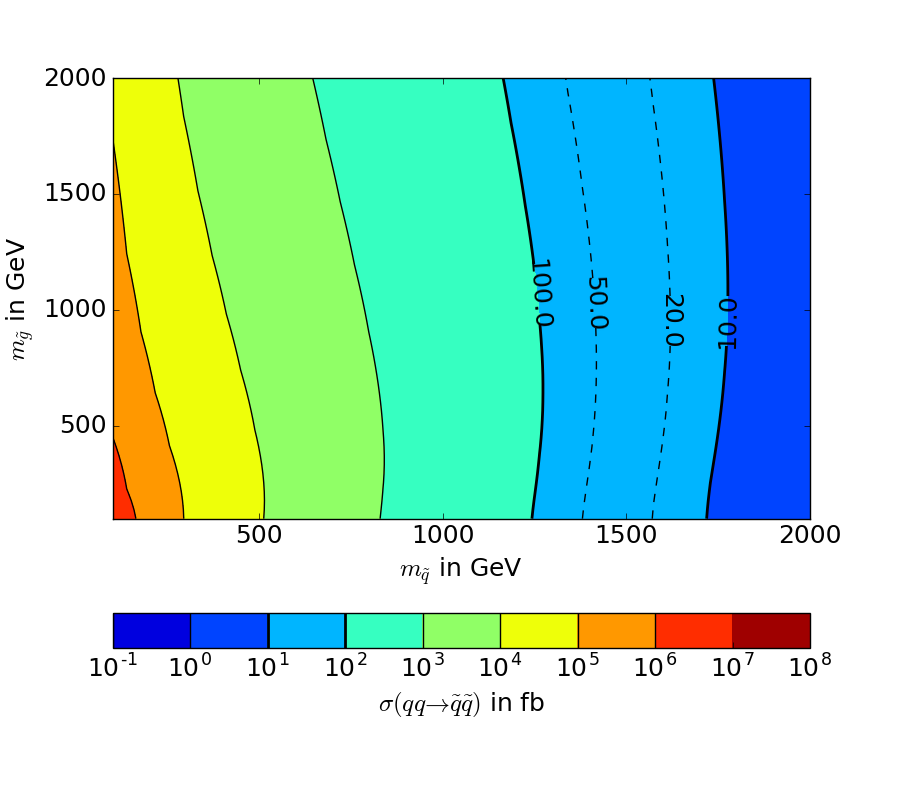
\includegraphics[scale=.6]{figures/contour_MSSM_squarks}
\caption{}
\end{center}
\end{figure}

\begin{figure}[!htpb]
\begin{center}
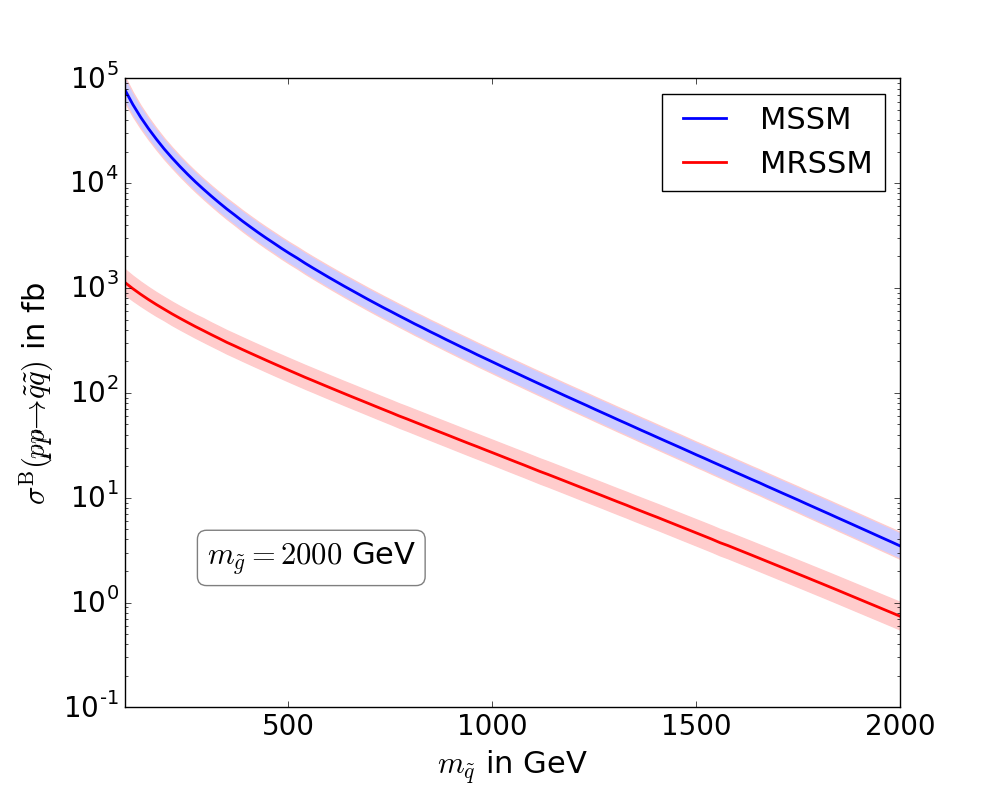
\includegraphics[scale=.5]{figures/MSSM+MRSSM_msg=2000}
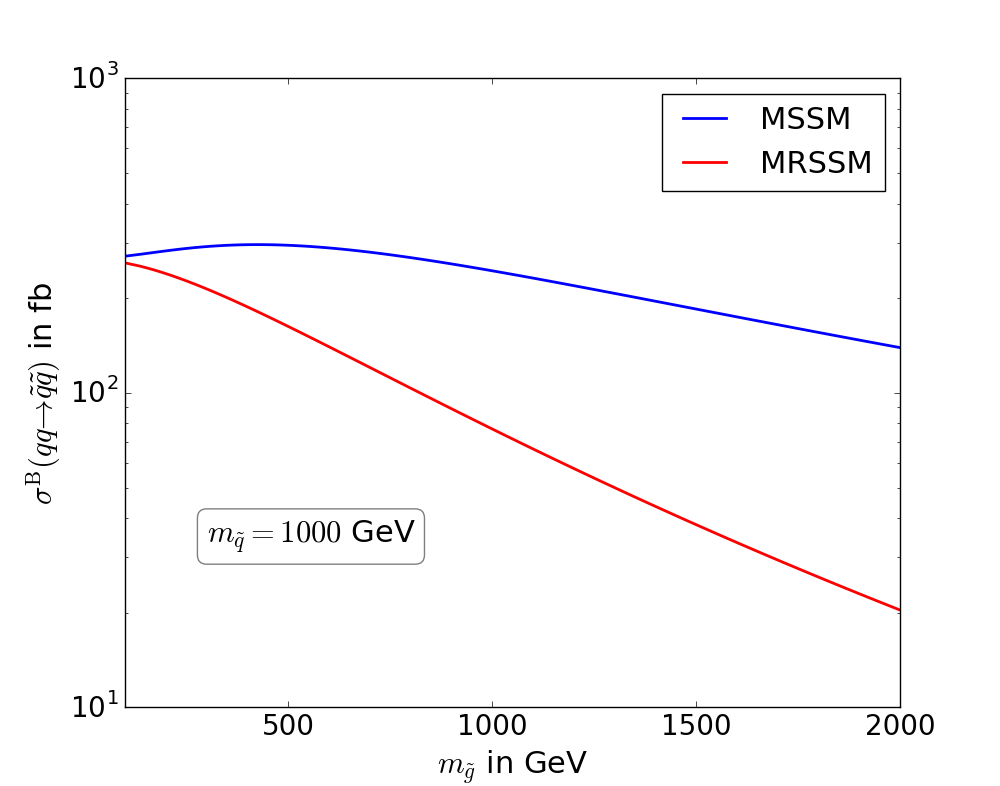
\includegraphics[scale=.5]{figures/MSSM+MRSSM_msq=1000}
\caption{add error bars}
\end{center}
\end{figure}

\newpage
\section{Renormalization of the MRSSM}
In order to improve the prediction of the cross section of the previous chapter one has to take quantum corrections into account. These are associated with loops in the corresponding Feynman diagrams. Computing these loop diagrams one might encounter infinities which arise from certain momentum configurations of the unspecified loop momentum. These infinities can be classified due to their origin. Infinities which are associated with loop momenta which tend to infinity are referred to as ultraviolet(UV) divergences. Infinities arising from loop momenta approaching zero can occur in loops with massless particles and are called infrared(IR) singularities. Furthermore there are collinear singularities with occur when a massless particle splits into two massless collinear particles.\\
These infinities are not physical and must therefore be removed to get sensible predictions. To this end one regularizes them to extract them from the quantity in question. UV-divergences can be removed by means of renormalization, i.e. counterterms are inserted into the Lagrangian to cancel UV-divergences. Infrared and collinear divergenves are removed by adding up all possible contributions which give rise to the considered observable.

\subsection{Regularization Schemes}\label{sec:RegSchemes}
\subsubsection*{Dimensional Regularization(DREG)}
Dimensional regularization(DREG) is a very common procedure for regularizing infinities which was devised by t'Hooft and Veltman~\cite{'tHooft:1972fi}. In this scheme loop momenta, gamma- and epsilon-tensors, phase space and fields are defined in $D$ dimensions. As in every regularization scheme a parameter with mass dimension needs to be introduced. In DREG that is the $\mu$ parameter which ensures that the loop integrals still have mass dimension 4:
\begin{align}
\int \frac{\mbox{d}^4p}{(2\pi)^4} \to \mu^{4-D} \int \frac{\mbox{d}^Dp}{(2\pi)^D}.
\end{align}
One often writes $D=4-2\epsilon$. Then the divergences of the loop integral manifest in $\frac{1}{\epsilon}$ poles.\\
However DREG suffers a flaw in supersymmetry. As the degrees of freedom for a massless gauge boson are $D-2$ but the degrees of freedom for its superpartner are 2 there is a mismatch if $D \neq 4$. As a consequence there are $2\epsilon$ degrees of freedom associated with the gluon\footnote{These degrees of freedom are identified with scalars and are therefore referred to as $\epsilon$ scalars} which do not have a supersymmetric partner. Therefore DREG violates supersymmetry.

\subsubsection*{Dimensional Reduction (DRED)}
Dimensional reduction (DRED) was introduced to rectify the imperfections of DREG, i.e. it preserves supersymmetry\footnote{It is not clear if DRED preserves supersymmetry at all orders in perturbation theory but it does preserve supersymmetry at the 1-loop level.}. DRED promotes only loop momenta to $D$ dimensions. All other quantities which are $D$ dimensional in DREG stay in 4 dimensions.\\
maybe refer to Collins: Renormalization


\subsection{Regularization Scheme Dependences}\label{sec:RegSchemeDep}
It is useful to introduce the effective action $\Gamma$ to discuss the subject of this and ensuing subchapters. A formal introduction of $\Gamma$ can be found in~\cite{Peskin}. In short $\Gamma$ can be viewed as a modification of the classical action $\Gamma_{cl} = \int \mathcal{L}_{cl}$ by quantum effects:
\begin{align}
\Gamma = \Gamma_{cl} + \mathcal{O}(\hbar)
\end{align}
This means that in addition to the vertices in the classical Lagrangian new vertices arise due to loop effects. As already suggested loop corrections might a priori not be finite and then need to be made finite by the addition of counterterms. For $\mathcal{O}(\hbar)$ corrections one writes
\begin{align}
\Gamma^{(\leq 1)} \to \Gamma^{(\leq 1)} + \Gamma^{(1),ct}
\end{align} 
These counterterms depend on the regularization (and renormalization) scheme. If one chooses to work with DREG supersymmetry will not be preserved at 1-loop order, i.e. $\Gamma^{(\leq 1)}_{DREG}$ is not supersymmetric. To maintain supersymmetry invariance of the renormalized effective action the counterterms will not only consist of supersymmetric counterterms $\Gamma^{(1),ct,sym}_{DREG}$ but also of counterterms restoring supersymmetry $\Gamma^{(1),ct,restore}_{DREG}$. 
\begin{align}
\Gamma^{(1),ct}_{DREG} = \Gamma^{(1),ct,sym}_{DREG} + \Gamma^{(1),ct,restore}_{DREG}
\end{align}
Fortunately a supersymmetry conserving regularization scheme (at 1-loop level) is given by DRED \cite{Hollik:2001cz}. One way to acquire supersymmetry restoring counterterms is therefore given by
\begin{align}
\Gamma^{(\leq 1)}_{DRED} + \Gamma^{(1),ct}_{DRED} \overset{!}{=} \Gamma^{(\leq 1)}_{DREG} + \Gamma^{(1),ct}_{DREG}.
\end{align}
Setting also the finite terms in $\Gamma^{(1),ct,sym}$ equal in DRED and DREG the choice of the supersymmetry restoring counterterms is fixed by:
\begin{align}
\Gamma^{(1),ct,restore}_{DREG} = \Gamma^{(\leq 1)}_{DRED} - \Gamma^{(\leq 1)}_{DREG}.\label{eq:GammaCtRestore}
\end{align} 
This way supersymmetry is preserved by the renormalization constants.\\ 
In the case of the MRSSM it will turn out that the only supersymmetry violation comes from correction associated with the gluon as already alluded to in \ref{sec:RegSchemes}. However supersymmetry restoring is always already included in $\delta Z^{\mathrm{DREG}}$. This is $\delta Z^{\mathrm{DREG}} = \delta Z^{\mathrm{DREG,sym}} + \delta Z^{\mathrm{trans}}$ where $\delta Z^{\mathrm{trans}} = \delta Z^{\mathrm{DREG}} - \delta Z^{\mathrm{DRED}}$ is the supersymmetry restoring renormalization constant. The only point where particularly care is required is the coupling: The  gauge coupling $g_s$ and the Yukawa coupling $\hat{g}_s$ receive different supersymmetry restoring counterterms. Therefore one has to make a difference between these couplings at 1-loop level. In order to match $g_s$ to the experimentally measured coupling it is renormalized in $\overline{\mathrm{MS}}$. The Yukawa coupling $\hat{g}_s$ therefore needs to be added with the difference of the supersymmetry restoring counterterms at 1-loop in order to be renormalized the same way.


%An alternative procedure is used in \cite{Beenakker:1996ch}, where only one supersymmetry restoring counterterm, which translates between the renormalized gauge coupling $g_s$ and the renormalized Yukawa coupling $\hat{G}_s$ is needed. That is possible because the only supersymmetry violation comes from the gauge sector. For a comprehensive discussion of this issue see [Philipp Vasros Diplomarbeit and the paper with Dominik]\\
%SUSY restoring is always already in $\delta Z^{DREG}$ included. Only important thing is the coupling: $g_s$ and $\hat{g}_s$ receive different SUSY restoring counterterm. Therefore one has to make a difference between these couplings at 1-loop level. In order to match $g_s$ to the experimentaly measured coupling it is renormalized in $\overline{\mathrm{MS}}$. The Yukawa coupling $\hat{g}_s$ therefore needs to be added with the difference of the SUSY-restoring counterterms at 1-loop in order to be renormalized the same way.


\subsection{On-Shell Renormalization}\label{sec:QuarkSE}
A part of the computation of NLO processes is the calculation of renormalization constants. The field and mass renormalization constants have been calculated in DREG in the on-shell scheme. This has the advantaged that when turning to the cross section no manipulation of the Green function to the S-matrix element has to be done. 

\subsubsection{The Quark Self-Energy}
The quark self-energy splits into contribution from the SM as well as a supersymmetric analogue which is already present in the MSSM.
\begin{figure}[!htbp]
\begin{center}
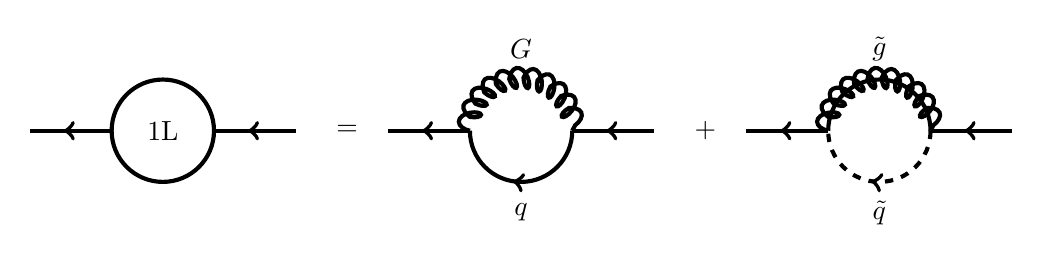
\begin{tikzpicture}[line width=1.5 pt, scale=1.3]
	\draw[fermionbar](180:1.3)--(180:0.5);
	\draw[fermionnoarrow] (-0.5,0) arc (180:0:.5);
	\draw[fermionnoarrow] (0.5,0) arc (0:-180:.5);	
	\node at (0,0) {1L};
	\draw[fermionbar](0:0.5)--(0:1.3);
	\node at (1.8,0) {=};
\begin{scope}[shift={(3.5,0)}]
	\draw[fermionbar](180:1.3)--(180:0.5);
	\draw[gluon] (-0.5,0) arc (180:0:.5);
	\node at (0,0.8) {$G$};
	\draw[fermion] (0.5,0) arc (0:-180:.5);
	\node at (0,-0.8) {$q$};	
	\draw[fermionbar](0:0.5)--(0:1.3);
	\node at (1.8,0) {+};
\end{scope}
\begin{scope}[shift={(7,0)}]
	\draw[fermionbar](180:1.3)--(180:0.5);
	\draw[gluon] (-0.5,0) arc (180:0:.5);
	\draw[fermionnoarrow] (-0.5,0) arc (180:0:.5);
	\node at (0,0.8) {$\tilde{g}$};
	\draw[scalar] (0.5,0) arc (0:-180:.5);
	\node at (0,-0.8) {$\tilde{q}$};	
	\draw[fermionbar](0:0.5)--(0:1.3);
\end{scope}
\end{tikzpicture}
\caption{diagrammatic contributions to the self-energy of the quark at 1-loop level}\label{fig:QuarkSelfEnergy}
\end{center}
\end{figure}\\
The 1-PI diagrams evaluate to
\begin{align}
i\Gamma^{1L}_{q_i\overline{q}_j} = i \frac{g_s^2}{16\pi^2}\delta_{ij} C(F) \left[ 2 \left( B_0(p^2,0,0) + B_1(p^2,0,0)-\frac{1}{2}\right)\slashed{p} - 2 B_1(p^2,m_{\tilde{g}}^2,m_{\tilde{q}}^2)\slashed{p}\right].
\end{align}
With the counterterm Feynman rule\\
\\
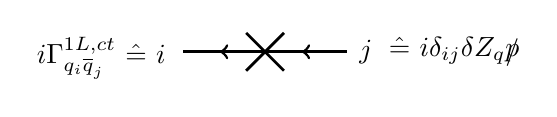
\begin{tikzpicture}[line width=1.0 pt, scale=0.8]
	\node at (-2.5,-0.1) {$i\Gamma^{1L,ct}_{q_i\overline{q}_j}\ \hat{=}\ i$};
\begin{scope}[shift={(0.1,0)}]	
	\draw[fermionbar] (-1.3,0) --(0,0);
	\draw[fermionnoarrow] (-0.3,0.3) -- (0.3,-0.3);
	\draw[fermionnoarrow] (-0.3,-0.3) -- (0.3,0.3);
	\draw[fermionbar] (0,0) --(1.3,0);
	\node at (1.6,0) {$j$};
	\node at (3,0) {$\hat{=}\ i\delta_{ij}\delta Z_q \slashed{p} $};	
\end{scope}
\end{tikzpicture}\\
and the on-shell renormalization condition
\begin{align}
\frac{\partial}{\partial \slashed{p}} \left[ \Re (\Gamma^{\mathrm{1L}}_{q_i\overline{q}_j}) + \Gamma^{\mathrm{1L,ct}}_{q_i\overline{q}_j}  \right]_{p^2 = 0} = 0
\end{align}
where $\Re (\hdots)$ denotes the real part of $\hdots$ one finds
\begin{align}
\delta Z_q = 2 C(F) \frac{g_s^2}{16\pi^2} \Re \left[ B_1(p^2,m_{\tilde{g}}^2,m_{\tilde{q}}^2) + \frac{1}{2} \right].
\end{align}
Doing the same calculation in DRED one finds that the second term in the squared brackets is absent. Therefore the transition counterterm between DREG and DRED is given by
\begin{align}
\delta Z_q^{\mathrm{trans}} = \delta Z_q^{\mathrm{DREG}} - \delta Z_q^{\mathrm{DRED}} = C(F) \frac{g_s^2}{16\pi^2}.\label{eq:QuarkSC}
\end{align}

\subsubsection{The Squark Self-Energy}
The contributions to the self-energy of the left- and right-handed squark are the same. Therefore to avoid unnecessary labeling $\Gamma_{\tilde{q}\tilde{q}^\dagger}$ stands in the following for $\Gamma_{\tilde{q}_L\tilde{q}_L^\dagger} = \Gamma_{\tilde{q}_R\tilde{q}_R^\dagger}$.
\begin{figure}[!htbp]
\begin{center}
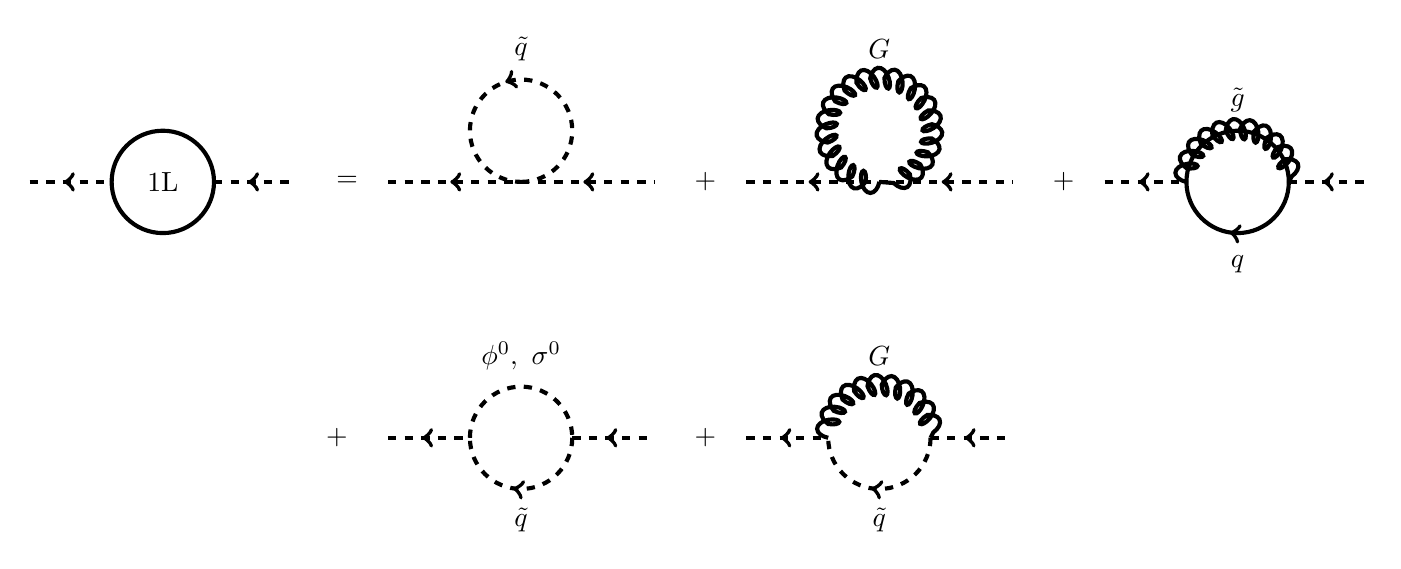
\begin{tikzpicture}[line width=1.5 pt, scale=1.3]
	\draw[scalarbar](180:1.3)--(180:0.5);
	\draw[fermionnoarrow] (-0.5,0) arc (180:0:.5);
	\draw[fermionnoarrow] (0.5,0) arc (0:-180:.5);	
	\node at (0,0) {1L};
	\draw[scalarbar](0:0.5)--(0:1.3);
	\node at (1.8,0) {=};
\begin{scope}[shift={(3.5,0)}]
	\draw[scalarbar](-1.3,0)--(0,0);
	\draw[scalarbar](0,0)--(1.3,0);
	\draw[scalar] (0,0) arc (-90:270:.5);
	\node at (0,1.3) {$\tilde{q}$};
	\node at (1.8,0) {+};
\end{scope}
\begin{scope}[shift={(7.0,0)}]
	\draw[scalarbar](-1.3,0)--(0,0);
	\draw[scalarbar](0,0)--(1.3,0);
	\draw[gluon] (0,0) arc (270:-90:.5);
	\node at (0,1.3) {$G$};
	\node at (1.8,0) {+};
\end{scope}
\begin{scope}[shift={(10.5,0)}]
	\draw[scalarbar](180:1.3)--(180:0.5);
	\draw[gluon] (-0.5,0) arc (180:0:.5);
	\draw[fermionnoarrow] (-0.5,0) arc (180:0:.5);
	\node at (0,0.8) {$\tilde{g}$};
	\draw[fermion] (0.5,0) arc (0:-180:.5);
	\node at (0,-0.8) {$q$};	
	\draw[scalarbar](0:0.5)--(0:1.3);
\end{scope}
\begin{scope}[shift={(3.5,-2.5)}]
	\node at (-1.8,0) {+};
	\draw[scalarbar](180:1.3)--(180:0.5);
	\draw[scalarnoarrow] (-0.5,0) arc (180:0:.5);
	\node at (0,0.8) {$\phi^0,\ \sigma^0$};
	\draw[scalar] (0.5,0) arc (0:-180:.5);
	\node at (0,-0.8) {$\tilde{q}$};	
	\draw[scalarbar](0:0.5)--(0:1.3);
	\node at (1.8,0) {+};
\end{scope}
\begin{scope}[shift={(7,-2.5)}]
	\draw[scalarbar](180:1.3)--(180:0.5);
	\draw[gluon] (-0.5,0) arc (180:0:.5);
	\node at (0,0.8) {$G$};
	\draw[scalar] (0.5,0) arc (0:-180:.5);
	\node at (0,-0.8) {$\tilde{q}$};	
	\draw[scalarbar](0:0.5)--(0:1.3);
\end{scope}
\end{tikzpicture}
\caption{diagrammatic contributions to the self-energy of the squark at 1-loop level}
\end{center}
\end{figure}\\
\begin{align}
i\Gamma^{1L}_{\tilde{q}_{i}\tilde{q}^\dagger_j} &= i \frac{g_s^2}{16\pi^2}\delta_{ij}C(F) \left[  A_0(m_{\tilde{q}}^2) + 0 - \left( 4A_0(m_{\tilde{g}}^2) + 4B_1(p^2,0,m_{\tilde{g}}^2)p^2 \right) \right.\nonumber\\
& \left.+ 4m_{\tilde{g}}^2B_0(p^2,m_{\phi^0}^2,m_{\tilde{q}}^2) - \left(2B_1(p^2,0,m_{\tilde{q}}^2)p^2 + B_0(p^2,0,m_{\tilde{q}}^2)(m_{\tilde{q}}^2+3p^2) \right) \right].
\end{align}
Suppressing $\delta_{AB}$ with $A,B = L,R$ which is present in the tree level propagator the counterterm Feynman rule is given by\\
\\
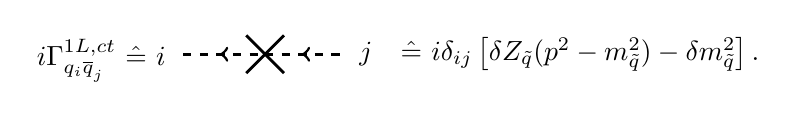
\begin{tikzpicture}[line width=1.0 pt, scale=0.8]
	\node at (-2.5,-0.1) {$i\Gamma^{1L,ct}_{q_i\overline{q}_j}\ \hat{=}\ i$};
\begin{scope}[shift={(0.1,0)}]	
	\draw[scalarbar] (-1.3,0) --(0,0);
	\draw[fermionnoarrow] (-0.3,0.3) -- (0.3,-0.3);
	\draw[fermionnoarrow] (-0.3,-0.3) -- (0.3,0.3);
	\draw[scalarbar] (0,0) --(1.3,0);
	\node at (1.6,0) {$j$};
	\node at (5,0) {$\hat{=}\ i\delta_{ij} \left[ \delta Z_{\tilde{q}}(p^2-m_{\tilde{q}}^2) - \delta m_{\tilde{q}}^2 \right] .$};	
\end{scope}
\end{tikzpicture}\\
The on-shell renormalization conditions read
\begin{align}
&\frac{\partial}{\partial p^2} \left[ \Re (\Gamma^{\mathrm{1L}}_{\tilde{q}_{i}\tilde{q}^\dagger_j}) + \Gamma^{\mathrm{1L,ct}}_{\tilde{q}_{i}\tilde{q}^\dagger_j}  \right]_{p^2 = m_{\tilde{q}}^2} = 0 && \left[ \Re (\Gamma^{\mathrm{1L}}_{\tilde{q}_{i}\tilde{q}^\dagger_j}) + \Gamma^{\mathrm{1L,ct}}_{\tilde{q}_{i}\tilde{q}^\dagger_j}  \right]_{p^2 = m_{\tilde{q}}^2} = 0.
\end{align}
This results in the following renormalization constants
\begin{align}
\delta Z_{\tilde{q}} &= \frac{g_s^2}{16\pi^2}C(F) \Re \left[ 4B_1(p^2,0,m_{\tilde{g}}^2) + 2B_1(B_1(p^2,0,m_{\tilde{q}}^2)) + 3B_0(p^2,0,m_{\tilde{q}}^2) \right.\nonumber\\
& + 4m_{\tilde{q}}^2 \frac{\partial}{\partial p^2}B_1(p^2,0,m_{\tilde{g}}^2) - 4m_{\tilde{g}}^2\frac{\partial}{\partial p^2}B_0(p^2,m_{\phi^0}^2,m_{\tilde{q}}^2) + 2m_{\tilde{q}}^2 \frac{\partial}{\partial p^2}B_1(p^2,0,m_{\tilde{q}}^2)\nonumber\\
& \left. + 4m_{\tilde{q}}^2 \frac{\partial}{\partial p^2}B_0(p^2,0,m_{\tilde{q}}^2)\right]_{p^2 = m_{\tilde{q}}^2}
\end{align}
\begin{align}
\delta m_{\tilde{q}}^2 = \frac{g_s^2}{16\pi^2}C(F)&\left[ A_0(m_{\tilde{q}}^2) - (4A_0(m_{\tilde{g}}^2) + 4B_1(m_{\tilde{q}}^2,0,m_{\tilde{g}}^2)m_{\tilde{q}}^2) + 4 m_{\tilde{g}}^2 B_0(m_{\tilde{q}}^2,m_{\phi^0}^2,m_{\tilde{q}}^2) \right.\nonumber\\
&\left. -(2B_1(m_{\tilde{q}}^2,0,m_{\tilde{q}}^2) m_{\tilde{q}}^2 + 4 B_0(m_{\tilde{q}}^2,0,m_{\tilde{q}}^2)m_{\tilde{q}}^2) \right]
\end{align}
The squark self-energy exhibits no regularization dependence. The transition counterterms are therefore 
\begin{align}
\delta Z_{\tilde{q}}^{\mathrm{trans}} = \delta m_{\tilde{q}}^{2\ \mathrm{trans}} = 0. \label{eq:SquarkSC}
\end{align}

\subsubsection{The Glunio Self-Energy}
The 4-spinor of the gluino comprises two Weyl spinors which describe very different particles.
\begin{align}
\tilde{g}^a = \begin{pmatrix}
\lambda^a \\
\overline{\chi}^a
\end{pmatrix}
\end{align}
The left-handed part $\lambda^a$ is associated with the superpartner of the gluon and therefore the "actual" gluino whereas the right-handed part $\overline{\chi}^a$ was introduced to assign a Dirac-mass to the gluino and is referred to as the octino.\\
From the Lagrangian \ref{eq:L_RSQCD} one can see that the couplings of the two particles are quite distinct. This is reflected by different field renormalization constants of the left- and right-handed part of the gluino.
\begin{figure}[!htbp]
\begin{center}
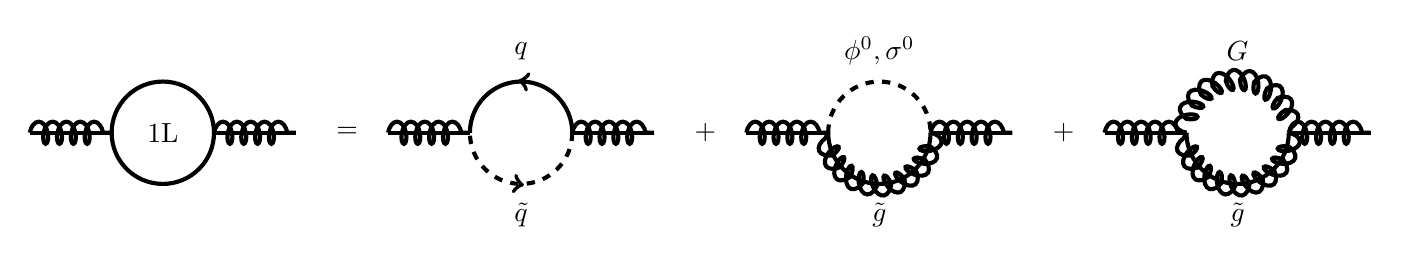
\begin{tikzpicture}[line width=1.5 pt, scale=1.3]
	\draw[fermionnoarrow](180:1.3)--(180:0.5);
	\draw[gluon](180:1.3)--(180:0.5);
	\draw[fermionnoarrow] (-0.5,0) arc (180:0:.5);
	\draw[fermionnoarrow] (0.5,0) arc (0:-180:.5);	
	\node at (0,0) {1L};
	\draw[fermionnoarrow](0:0.5)--(0:1.3);
	\draw[gluon](0:0.5)--(0:1.3);
	\node at (1.8,0) {=};
\begin{scope}[shift={(3.5,0)}]
	\draw[fermionnoarrow](180:1.3)--(180:0.5);
	\draw[gluon](180:1.3)--(180:0.5);
	\draw[fermionbar] (-0.5,0) arc (180:0:.5);
	\node at (0,0.8) {$q$};
	\draw[scalarbar] (0.5,0) arc (0:-180:.5);
	\node at (0,-0.8) {$\tilde{q}$};	
	\draw[fermionnoarrow](0:0.5)--(0:1.3);
	\draw[gluon](0:0.5)--(0:1.3);
	\node at (1.8,0) {+};
\end{scope}
\begin{scope}[shift={(7.0,0)}]
	\draw[gluon](180:1.3)--(180:0.5);
	\draw[fermionnoarrow](180:1.3)--(180:0.5);
	\draw[scalarnoarrow] (-0.5,0) arc (180:0:.5);
	\node at (0,0.8) {$\phi^0,\sigma^0$};
	\draw[fermionnoarrow] (0.5,0) arc (0:-180:.5);
	\draw[gluon] (0.5,0) arc (0:-180:.5);
	\node at (0,-0.8) {$\tilde{g}$};	
	\draw[gluon](0:0.5)--(0:1.3);
	\draw[fermionnoarrow](0:0.5)--(0:1.3);
	\node at (1.8,0) {+};
\end{scope}
\begin{scope}[shift={(10.5,0)}]
	\draw[gluon](180:1.3)--(180:0.5);
	\draw[fermionnoarrow](180:1.3)--(180:0.5);
	\draw[gluon] (-0.5,0) arc (180:0:.5);
	\node at (0,0.8) {$G$};
	\draw[fermionnoarrow] (0.5,0) arc (0:-180:.5);	
	\draw[gluon] (0.5,0) arc (0:-180:.5);
	\node at (0,-0.8) {$\tilde{g}$};	
	\draw[fermionnoarrow](0:0.5)--(0:1.3);
	\draw[gluon](0:0.5)--(0:1.3);
\end{scope}
\end{tikzpicture}
\caption{diagrammatic contributions to the self-energy of the squark at 1-loop level}
\end{center}
\end{figure}
As for the quarks the fermion (and momentum) flow is from the right to the left.
\begin{align}
i\Gamma^{1L}_{\tilde{g}^a \overline{\tilde{g}}^b} &= i \frac{g_s^2}{16\pi^2}\delta_{ab} \left[-4T(F)\left( (n_f-1) B_1(p^2,0,m_{\tilde{q}}^2) + B_1(p^2,m_t^2,m_{\tilde{q}}^2) \right)P_L \slashed{p} \right.\nonumber\\
& + C(A)\left( (B_0(p^2,m_{\tilde{g}}^2,m_{\phi^0}^2) - B_0(p^2,m_{\tilde{g}}^2,m_{\sigma^0}^2))m_{\tilde{g}} - (B_1(p^2,m_{\tilde{g}}^2,m_{\phi^0}^2) + B_1(p^2,m_{\tilde{g}}^2,m_{\sigma^0}^2))\slashed{p} \right) \nonumber\\
&\left.+ C(A)\left( (2 - 4 B_0(p^2,0,m_{\tilde{g}}^2)) m_{\tilde{g}} - (1-2(B_0(p^2,0,m_{\tilde{g}}^2) + B_1(p^2,0,m_{\tilde{g}}^2)))\slashed{p} \right)\right]
\end{align}
Where $n_f = 6$ is the number of quark flavors.\\
The counterterm Feynman rule reads\\
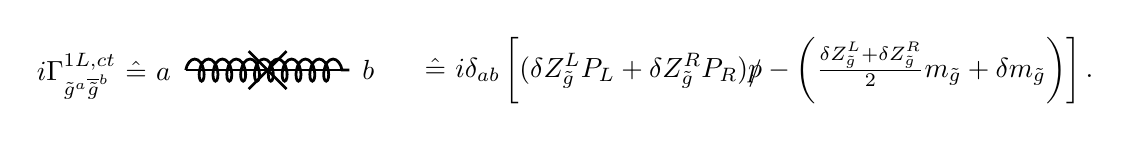
\begin{tikzpicture}[line width=1.0 pt, scale=0.8]
	\node at (-2.5,-0.1) {$i\Gamma^{1L,ct}_{\tilde{g}^a \overline{\tilde{g}}^b}\ \hat{=}\ a$};
\begin{scope}[shift={(0.1,0)}]	
	\draw[gluon] (-1.3,0) --(1.3,0);
	\draw[fermionnoarrow] (-0.3,0.3) -- (0.3,-0.3);
	\draw[fermionnoarrow] (-0.3,-0.3) -- (0.3,0.3);
	\draw[fermionnoarrow] (-1.3,0) --(1.3,0);
	\node at (1.6,0) {$b$};
	\node at (7.8,0) {$\hat{=}\ i\delta_{ab}\left[ (\delta Z_{\tilde{g}}^L P_L + \delta Z_{\tilde{g}}^R P_R)\slashed{p} - \left(\frac{\delta Z_{\tilde{g}}^L+\delta Z_{\tilde{g}}^R}{2} m_{\tilde{g}} +\delta m_{\tilde{g}}\right) \right]. $};	
\end{scope}
\end{tikzpicture}\\
The on-shell renormalization conditions for the fields are
\begin{align}
& \frac{\partial}{\partial (P_L\slashed{p})} \left[ \Re (\Gamma^{\mathrm{1L}}_{\tilde{g}^a \overline{\tilde{g}}^b}) + \Gamma^{\mathrm{1L,ct}}_{\tilde{g}^a \overline{\tilde{g}}^b}  \right]_{\slashed{p} = m_{\tilde{g}}} = 0
&& \frac{\partial}{\partial (P_R\slashed{p})} \left[ \Re (\Gamma^{\mathrm{1L}}_{\tilde{g}^a \overline{\tilde{g}}^b}) + \Gamma^{\mathrm{1L,ct}}_{\tilde{g}^a \overline{\tilde{g}}^b}  \right]_{\slashed{p} = m_{\tilde{g}}} = 0
\end{align}
where the derivative of $\Sigma = \Sigma^{VL}P_L\slashed{p} + \Sigma^{VR}P_R\slashed{p} + \Sigma^{SL}P_L + \Sigma^{SR}P_R$ with respect to $P_A\slashed{p}$ \\
($A = L,R$) is defined by
\begin{align}
\left.\frac{\partial}{\partial (P_A\slashed{p})} \Sigma\right|_{\slashed{p} = m} = \Sigma^{VA} + \frac{\partial}{\partial p^2} \left( m^2 \Sigma^{VL} + m^2 \Sigma^{VR} + m \Sigma^{SL} + m \Sigma^{SR}\right).
\end{align}
This leads to the following renormalization constants
\begin{align}
\delta Z_{\tilde{g}}^L &= \frac{g_s^2}{16\pi^2}\Re \left[ 4T(F)\left( (n_f-1) B_1(m_{\tilde{g}}^2,0,m_{\tilde{q}}^2) + B_1(m_{\tilde{g}}^2,m_t^2,m_{\tilde{q}}^2) \right) \right.\nonumber\\
&+C(A) (B_1(m_{\tilde{g}}^2,m_{\tilde{g}}^2,m_{\phi^0}^2) + B_1(m_{\tilde{g}}^2,m_{\tilde{g}}^2,m_{\sigma^0}^2))\nonumber\\
&+C(A)(1-2(B_0(m_{\tilde{g}}^2,0,m_{\tilde{g}}^2) + B_1(m_{\tilde{g}}^2,0,m_{\tilde{g}}^2)))\nonumber\\
&+ 4T(F) m_{\tilde{g}}^2 \frac{\partial}{\partial p^2} \left( ((n_f-1))  B_1(p^2,0,m_{\tilde{q}}^2) +  B_1(p^2,m_t^2,m_{\tilde{q}}^2) \right)\nonumber\\
&-2 C(A) m_{\tilde{g}} \frac{\partial}{\partial p^2} \left( B_0(p^2,m_{\tilde{g}}^2,m_{\phi^0}^2)-B_0(p^2,m_{\tilde{g}}^2,m_{\sigma^0}^2) - B_1(p^2,m_{\tilde{g}}^2,m_{\phi^0}^2) - B_1(p^2,m_{\tilde{g}}^2,m_{\sigma^0}^2) \right)\nonumber\\
&-4 C(A) m_{\tilde{g}}^2 \frac{\partial}{\partial p^2} \left.\left( -B_0(p^2,0,m_{\tilde{g}}^2) + B_0(p^2,0,m_{\tilde{g}}^2) \right)\right]_{p^2=m_{\tilde{g}}^2}
\end{align}
and 
\begin{align}
\delta Z_{\tilde{g}}^R &= \frac{g_s^2}{16\pi^2}\Re \left[C(A) (B_1(m_{\tilde{g}}^2,m_{\tilde{g}}^2,m_{\phi^0}^2) + B_1(m_{\tilde{g}}^2,m_{\tilde{g}}^2,m_{\sigma^0}^2)) \right.\nonumber\\
&+C(A)(1-2(B_0(m_{\tilde{g}}^2,0,m_{\tilde{g}}^2) + B_1(m_{\tilde{g}}^2,0,m_{\tilde{g}}^2)))\nonumber\\
&+ 4T(F) m_{\tilde{g}}^2 \frac{\partial}{\partial p^2} \left( ((n_f-1))  B_1(p^2,0,m_{\tilde{q}}^2) +  B_1(p^2,m_t^2,m_{\tilde{q}}^2) \right)\nonumber\\
&-2 C(A) m_{\tilde{g}} \frac{\partial}{\partial p^2} \left( B_0(p^2,m_{\tilde{g}}^2,m_{\phi^0}^2)-B_0(p^2,m_{\tilde{g}}^2,m_{\sigma^0}^2) - B_1(p^2,m_{\tilde{g}}^2,m_{\phi^0}^2) - B_1(p^2,m_{\tilde{g}}^2,m_{\sigma^0}^2) \right)\nonumber\\
&-4 C(A) m_{\tilde{g}}^2 \frac{\partial}{\partial p^2} \left.\left( -B_0(p^2,0,m_{\tilde{g}}^2) + B_0(p^2,0,m_{\tilde{g}}^2) \right)\right]_{p^2=m_{\tilde{g}}^2}.
\end{align}
As for the quark there are constant terms amid the Passarino-Veltman integrals. These arise only in DREG and not in DRED. The transition counterterms are
\begin{align}
\delta Z_{\tilde{g}}^{A\ \mathrm{trans}} = \delta Z_{\tilde{g}}^{A\ \mathrm{DREG}} - \delta Z_{\tilde{g}}^{A\ \mathrm{DRED}} = C(A) \frac{g_s^2}{16\pi^2}\label{eq:GluinoSC}
\end{align}
for $A = L,R$. The gluino mass counterterm is ascertained by the condition
\begin{align}
\left[ \Re (\Gamma^{\mathrm{1L}}_{\tilde{g}^a \overline{\tilde{g}}^b}) + \Gamma^{\mathrm{1L,ct}}_{\tilde{g}^a \overline{\tilde{g}}^b}  \right]_{\slashed{p} = m_{\tilde{g}}} = 0
\end{align}
which is equivalent to 
\begin{align}
\delta m_{\tilde{g}} = \Re\left( m_{\tilde{g}}\frac{\Sigma^{VL}+\Sigma^{VR}}{2} + \frac{\Sigma^{SL}+\Sigma^{SR}}{2} \right)
\end{align}
and yields
\begin{align}
\delta m_{\tilde{g}} &= \frac{g_s^2}{16\pi^2} m_{\tilde{g}}^2\ \Re \left[ -2T(F) \left( (n_f-1)B_1(m_{\tilde{g}}^2,0,m_{\tilde{q}}^2) + B_1(m_{\tilde{g}}^2,m_t^2,m_{\tilde{q}}^2) \right) \right.\nonumber\\
& + C(A) \left( B_0(m_{\tilde{g}}^2,m_{\tilde{g}}^2,m_{\phi^0}^2) - B_0(m_{\tilde{g}}^2,m_{\tilde{g}}^2,m_{\sigma^0}^2) - B_1(m_{\tilde{g}}^2,m_{\tilde{g}}^2,m_{\phi^0}^2) -
B_1(m_{\tilde{g}}^2,m_{\tilde{g}}^2,m_{\sigma^0}^2) \right)\nonumber\\
& + C(A) \left.\left( 1 - 2 B_0(m_{\tilde{g}}^2,0,m_{\tilde{g}}^2) + 2 B_1(m_{\tilde{g}}^2,0,m_{\tilde{g}}^2) \right)\right].
\end{align}
Again there is a transition counterterm 
\begin{align}
\delta m_{\tilde{g}}^{\mathrm{trans}} = \delta m_{\tilde{g}}^{\mathrm{DREG}} - \delta m_{\tilde{g}}^{\mathrm{DRED}} = C(A) \frac{g_s^2}{16\pi^2} m_{\tilde{g}}.
\end{align}


\subsection{Renormalization of the Gauge Coupling}
The gauge coupling $g_s$ is renormalized in the $\overline{\mathrm{MS}}$-scheme with the modification that additional logarithms are substracted. This is to decouple heavy particles from the running of $\alpha_s = \frac{g_s^2}{4\pi}$. This renormalization procedure allows to adopt the experimental values of $\alpha_s$ from the PDF's. The running due to effects of heavy particles is then encoded in the logarithms of $\delta g_s$.\\
Extracting $\delta g_s$ from the quark-quark-gluon vertex requires not only the computation of $i\Gamma^{1L}_{q_i\overline{q}_jG^a}$ but also the (re)evaluation  of the auxiliary field renormalization constants $\delta Z_q^{\mathrm{aux}}$ and $\delta Z_G^{\mathrm{aux}}$. These will not be the same as the on-shell field renormalization.

\subsubsection{The Quark Self-Energy Revisited}
The quark self-energy has two contribution which are shown in figure \ref{fig:QuarkSelfEnergy}. The first one corresponds to light particles the second one to heavy particles: $i\Gamma^{\mathrm{1L}}_{q_i\overline{q}_j} = i\Gamma^{\mathrm{1L,light}}_{q_i\overline{q}_j} + i\Gamma^{\mathrm{1L,heavy}}_{q_i\overline{q}_j}$. For light particles only the UV-divergent part is kept. For heavy particles also the $\mu$-dependent terms are kept:
\begin{align}
i\Gamma^{\mathrm{1L,light}}_{q_i\overline{q}_j}|_{\mathrm{UV-div}} &= i \frac{g_s^2}{16\pi^2}\delta_{ij} \slashed{p} C(F) \frac{1}{\epsilon_{\mathrm{UV}}}\\
i\Gamma^{\mathrm{1L,heavy}}_{q_i\overline{q}_j}|_{\mathrm{UV-div,\mu-dep}} &= i \frac{g_s^2}{16\pi^2}\delta_{ij} \slashed{p} C(F)\left( \frac{1}{\epsilon_{\mathrm{UV}}} -\ln\frac{m_{\tilde{q}}^2}{\mu^2} \right)
\end{align}
The renormalization constant for the evaluation of $\delta g_s$ is determined by the condition
\begin{align}
\frac{\partial}{\partial \slashed{p}} \left[  \Gamma^{\mathrm{1L,light}}_{q_i\overline{q}_j}|_{\mathrm{UV-div}} + \Gamma^{\mathrm{1L,heavy}}_{q_i\overline{q}_j}|_{\mathrm{UV-div,\mu-dep}} + \Gamma^{\mathrm{1L,ct}}_{q_i\overline{q}_j}  \right]_{p^2 = 0} = 0
\end{align}
and computes to
\begin{align}
\delta Z_q^{\mathrm{aux}} = -\frac{g_s^2}{16\pi^2} C(F)\left[\left( \frac{1}{\epsilon_{\mathrm{UV}}} \right) + \left( \frac{1}{\epsilon_{\mathrm{UV}}} - \ln\frac{m_{\tilde{q}}^2}{\mu^2} \right) \right]
\end{align}
The first curved bracket corresponds to contributions from light particles in the loop whereas the second curved bracket corresponds to contributions from heavy particles in the loop.

\subsubsection{The Gluon Self-Energy}
As for the quark self-energy there are again contributions to the self-energy originating from light and heavy particles. As for the quark only specific terms are kept in calculating the auxiliary renormalization constants.  
\begin{figure}[!htbp]
\begin{center}
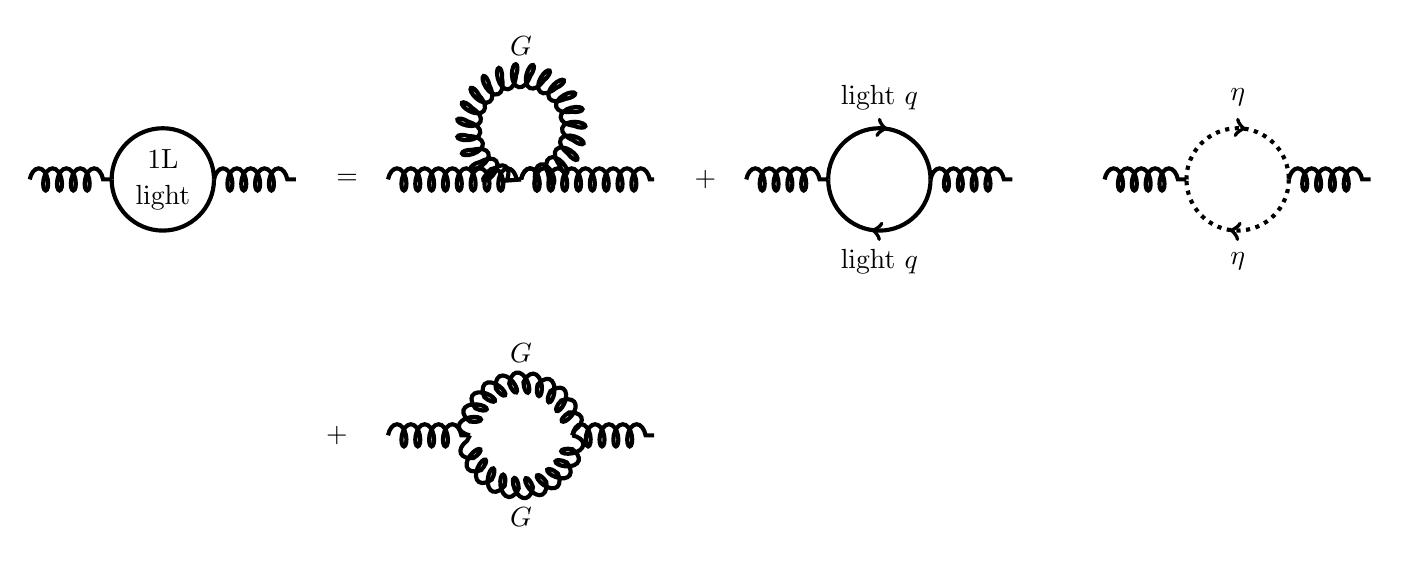
\begin{tikzpicture}[line width=1.5 pt, scale=1.3]
	\draw[gluon](180:1.3)--(180:0.5);
	\draw[fermionnoarrow] (-0.5,0) arc (180:0:.5);
	\draw[fermionnoarrow] (0.5,0) arc (0:-180:.5);	
	\node at (0,0.2) {1L};
	\node at (0,-0.18) {light};
	\draw[gluon](0:0.5)--(0:1.3);
	\node at (1.8,0) {=};
\begin{scope}[shift={(3.5,0)}]
	\draw[gluon](-1.3,0)--(0,0);
	\draw[gluon](0,0)--(1.3,0);
	\draw[gluon] (0,0) arc (-90:270:.5);
	\node at (0,1.3) {$G$};
	\node at (1.8,0) {+};
\end{scope}
\begin{scope}[shift={(7.0,0)}]
	\draw[gluon](180:1.3)--(180:0.5);
	\draw[fermion] (-0.5,0) arc (180:0:.5);
	\node at (0,0.8) {light $q$};
	\draw[fermion] (0.5,0) arc (0:-180:.5);
	\node at (0,-0.8) {light $q$};	
	\draw[gluon](0:0.5)--(0:1.3);
\end{scope}
\begin{scope}[shift={(10.5,0)}]
	\draw[gluon](180:1.3)--(180:0.5);
	\draw[ghost] (-0.5,0) arc (180:0:.5);
	\node at (0,0.8) {$\eta$};
	\draw[ghost] (0.5,0) arc (0:-180:.5);
	\node at (0,-0.8) {$\eta$};	
	\draw[gluon](0:0.5)--(0:1.3);
\end{scope}
\begin{scope}[shift={(3.5,-2.5)}]
	\node at (-1.8,0) {+};
	\draw[gluon](180:1.3)--(180:0.5);
	\draw[gluon] (-0.5,0) arc (180:0:.5);
	\node at (0,0.8) {$G$};
	\draw[gluon] (0.5,0) arc (0:-180:.5);
	\node at (0,-0.8) {$G$};	
	\draw[gluon](0:0.5)--(0:1.3);
\end{scope}
\end{tikzpicture}
\caption{contribution to the self-energy of the gluon originating from light particles}\label{fig:lightGluonSelfEnergy}
\end{center}
\end{figure}
\begin{align}
i\Gamma^{\mathrm{1L,light}}_{G_\mu^a G_\nu^b}|_{\mathrm{UV-div}} &= i\frac{g_s^2}{16\pi^2 \epsilon_{\mathrm{UV}}}\delta_{ab} \left[ 0 - \frac{4 (n_{f}-1)}{3} T(F) (p^2g^{\mu\nu}-p^\mu p^\nu) + \frac{C(A)}{12}(p^2g^{\mu\nu} + 2 p^\mu p^\nu) \right.\nonumber\\
&+\left. \frac{C(A)}{12}(19 p^2g^{\mu\nu} - 22 p^\mu p^\nu) \right]\nonumber\\
&=i\frac{g_s^2}{16\pi^2 \epsilon_{\mathrm{UV}}}\delta_{ab} \left[ - \frac{4 (n_{f}-1)}{3} T(F) + \frac{5}{3} C(A) \right](p^2g^{\mu\nu}-p^\mu p^\nu)
\end{align}
\begin{figure}[!htbp]
\begin{center}
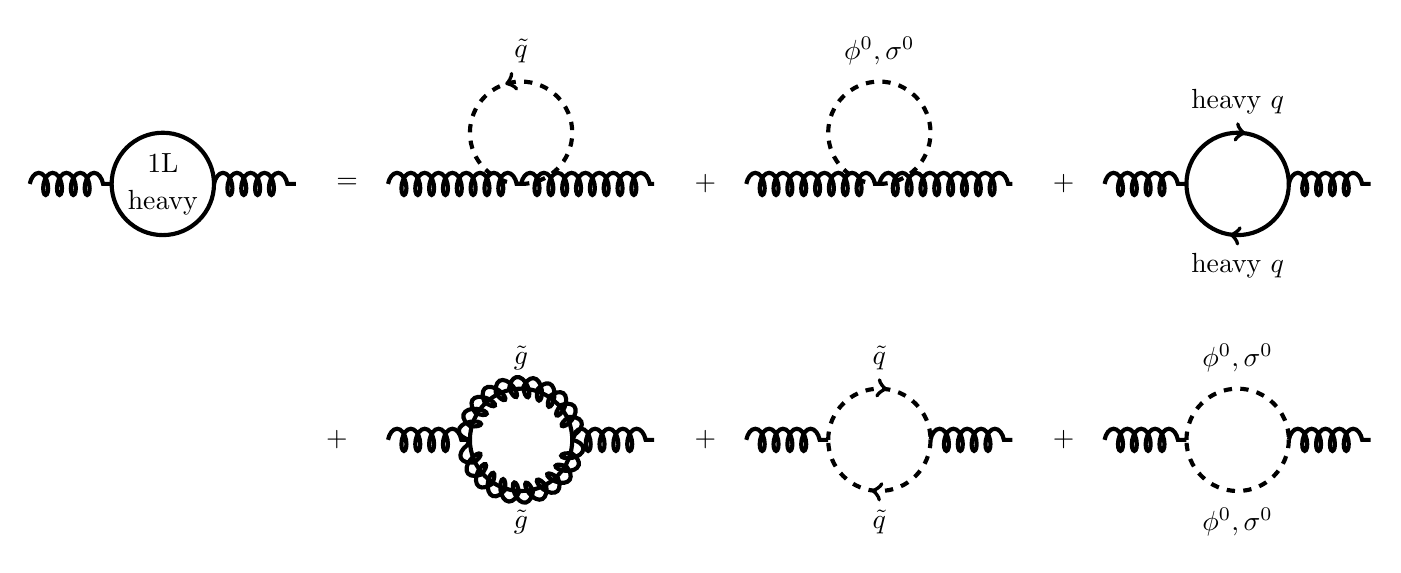
\begin{tikzpicture}[line width=1.5 pt, scale=1.3]
	\draw[gluon](180:1.3)--(180:0.5);
	\draw[fermionnoarrow] (-0.5,0) arc (180:0:.5);
	\draw[fermionnoarrow] (0.5,0) arc (0:-180:.5);	
	\node at (0,0.2) {1L};
	\node at (0,-0.18) {heavy};
	\draw[gluon](0:0.5)--(0:1.3);
	\node at (1.8,0) {=};
\begin{scope}[shift={(3.5,0)}]
	\draw[gluon](-1.3,0)--(0,0);
	\draw[gluon](0,0)--(1.3,0);
	\draw[scalar] (0,0) arc (-90:270:.5);
	\node at (0,1.3) {$\tilde{q}$};
	\node at (1.8,0) {+};
\end{scope}
\begin{scope}[shift={(7.0,0)}]
	\draw[gluon](-1.3,0)--(0,0);
	\draw[gluon](0,0)--(1.3,0);
	\draw[scalarnoarrow] (0,0) arc (-90:270:.5);
	\node at (0,1.3) {$\phi^0,\sigma^0$};
	\node at (1.8,0) {+};
\end{scope}
\begin{scope}[shift={(10.5,0)}]
	\draw[gluon](180:1.3)--(180:0.5);
	\draw[fermion] (-0.5,0) arc (180:0:.5);
	\node at (0,0.8) {heavy $q$};
	\draw[fermion] (0.5,0) arc (0:-180:.5);
	\node at (0,-0.8) {heavy $q$};	
	\draw[gluon](0:0.5)--(0:1.3);
\end{scope}
\begin{scope}[shift={(3.5,-2.5)}]
	\node at (-1.8,0) {+};
	\draw[gluon](180:1.3)--(180:0.5);
	\draw[gluon] (-0.5,0) arc (180:0:.5);
	\draw[fermionnoarrow] (-0.5,0) arc (180:0:.5);
	\node at (0,0.8) {$\tilde{g}$};
	\draw[gluon] (0.5,0) arc (0:-180:.5);
	\draw[fermionnoarrow] (0.5,0) arc (0:-180:.5);
	\node at (0,-0.8) {$\tilde{g}$};	
	\draw[gluon](0:0.5)--(0:1.3);
	\node at (1.8,0) {+};
\end{scope}
\begin{scope}[shift={(7,-2.5)}]
	\draw[gluon](180:1.3)--(180:0.5);
	\draw[scalar] (-0.5,0) arc (180:0:.5);
	\node at (0,0.8) {$\tilde{q}$};
	\draw[scalar] (0.5,0) arc (0:-180:.5);
	\node at (0,-0.8) {$\tilde{q}$};	
	\draw[gluon](0:0.5)--(0:1.3);
	\node at (1.8,0) {+};
\end{scope}
\begin{scope}[shift={(10.5,-2.5)}]
	\draw[gluon](180:1.3)--(180:0.5);
	\draw[scalarnoarrow] (-0.5,0) arc (180:0:.5);
	\node at (0,0.8) {$\phi^0,\sigma^0$};
	\draw[scalarnoarrow] (0.5,0) arc (0:-180:.5);
	\node at (0,-0.8) {$\phi^0,\sigma^0$};	
	\draw[gluon](0:0.5)--(0:1.3);
\end{scope}
\end{tikzpicture}
\caption{contribution to the self-energy of the gluon originating from heavy particles, in the last diagram either $\phi^0$ or $\sigma^0$ are running in the loop}
\end{center}
\end{figure}
The heavy particle contributions are given by\\
\begin{align}
i\Gamma^{\mathrm{1L,heavy}}_{G_\mu^a G_\nu^b}|_{\mathrm{UV-div, \mu-dep}} &= i\frac{g_s^2}{16\pi^2}\delta_{ab} \left[ - 4 T(F)n_f \left( \frac{1}{\epsilon_{\mathrm{UV}}} - \ln \frac{m_{\tilde{q}}^2}{\mu2} \right)m_{\tilde{q}}^2 g^{\mu\nu} - C(A) \left( \frac{1}{\epsilon_{\mathrm{UV}}} - \ln \frac{m_{\phi^0}^2}{\mu2} \right)m_{\phi^0}^2 g^{\mu\nu} \right.\nonumber\\
&- C(A) \left( \frac{1}{\epsilon_{\mathrm{UV}}} - \ln \frac{m_{\sigma^0}^2}{\mu2} \right)m_{\sigma^0}^2 g^{\mu\nu} - \frac{4}{3}T(F)\left( \frac{1}{\epsilon_{\mathrm{UV}}} - \ln \frac{m_t^2}{\mu2} \right)(p^2g^{\mu\nu}-p^\mu p^\nu)\nonumber\\
& - \frac{4}{3} C(A) \left( \frac{1}{\epsilon_{\mathrm{UV}}} - \ln \frac{m_{\tilde{g}}^2}{\mu2} \right)(p^2g^{\mu\nu}-p^\mu p^\nu)\nonumber\\
& -\frac{2}{3}T(F) n_f \left( \frac{1}{\epsilon_{\mathrm{UV}}} - \ln \frac{m_{\tilde{q}}^2}{\mu2} \right)(p^2g^{\mu\nu}-p^\mu p^\nu) + 4T(F)n_f \left( \frac{1}{\epsilon_{\mathrm{UV}}} - \ln \frac{m_{\tilde{q}}^2}{\mu2} \right)m_{\tilde{q}}^2 g^{\mu\nu} \nonumber\\
&-\frac{1}{6} C(A) \left( \frac{1}{\epsilon_{\mathrm{UV}}} - \ln \frac{m_{\phi^0}^2}{\mu2} \right)(p^2g^{\mu\nu}-p^\mu p^\nu) + C(A) \left( \frac{1}{\epsilon_{\mathrm{UV}}} - \ln \frac{m_{\phi^0}^2}{\mu2} \right)m_{\phi^0}^2 g^{\mu\nu} \nonumber\\
&\left.-\frac{1}{6} C(A) \left( \frac{1}{\epsilon_{\mathrm{UV}}} - \ln \frac{m_{\phi^0}^2}{\mu2} \right)(p^2g^{\mu\nu}-p^\mu p^\nu) + C(A) \left( \frac{1}{\epsilon_{\mathrm{UV}}} - \ln \frac{m_{\phi^0}^2}{\mu2} \right)m_{\phi^0}^2 g^{\mu\nu}\right]\nonumber\\
&= i\frac{g_s^2}{16\pi^2}\delta_{ab} \left[- \frac{4}{3}T(F)\left( \frac{1}{\epsilon_{\mathrm{UV}}} - \ln \frac{m_t^2}{\mu2} \right)(p^2g^{\mu\nu}-p^\mu p^\nu)\right.\nonumber\\
& - \frac{4}{3} C(A) \left( \frac{1}{\epsilon_{\mathrm{UV}}} - \ln \frac{m_{\tilde{g}}^2}{\mu2} \right)(p^2g^{\mu\nu}-p^\mu p^\nu)\nonumber\\
& -\frac{2}{3}T(F) n_f \left( \frac{1}{\epsilon_{\mathrm{UV}}} - \ln \frac{m_{\tilde{q}}^2}{\mu2} \right)(p^2g^{\mu\nu}-p^\mu p^\nu) \nonumber\\
&-\frac{1}{6} C(A) \left( \frac{1}{\epsilon_{\mathrm{UV}}} - \ln \frac{m_{\phi^0}^2}{\mu2} \right)(p^2g^{\mu\nu}-p^\mu p^\nu)  \nonumber\\
&\left.-\frac{1}{6} C(A) \left( \frac{1}{\epsilon_{\mathrm{UV}}} - \ln \frac{m_{\phi^0}^2}{\mu2} \right)(p^2g^{\mu\nu}-p^\mu p^\nu) \right]
\end{align}
The counterterm Feynman rule for the gluon propagator is\\
\\
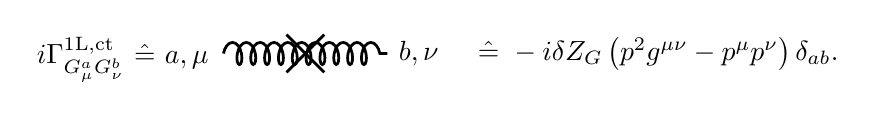
\begin{tikzpicture}[line width=1.0 pt, scale=0.8]
	\node at (-2.5,-0.1) {$i\Gamma^{\mathrm{1L,ct}}_{G_\mu^a G_\nu^b}\ \hat{=}\ a,\mu$};
\begin{scope}[shift={(0.4,0)}]	
	\draw[gluon] (-1.3,0) --(1.3,0);
	\draw[fermionnoarrow] (-0.3,0.3) -- (0.3,-0.3);
	\draw[fermionnoarrow] (-0.3,-0.3) -- (0.3,0.3);
	\node at (1.8,0) {$b,\nu$};
	\node at (5.6,0) {$\hat{=}\ -i \delta Z_G\left(p^2 g^{\mu\nu} - p^\mu p^\nu \right)\delta_{ab}.$};	
\end{scope}
\end{tikzpicture}\\
The renormalization condition for $\delta Z^{\mathrm{aux}}_G$ reads
\begin{align}
 \Gamma^{\mathrm{1L,light}}_{G_\mu^a G_\nu^b}|_{\mathrm{UV-div}} + \Gamma^{\mathrm{1L,heavy}}_{G_\mu^a G_\nu^b}|_{\mathrm{UV-div,\mu-dep}} - \delta Z_G^{\mathrm{aux}}\left(p^2 g^{\mu\nu} - p^\mu p^\nu \right)\delta_{ab} = 0
\end{align}
and yields
\begin{align}
\delta Z^{aux}_G &= \frac{g_s^2}{16\pi^2} \left\{\left[-\frac{4}{3}T(F)(n_f-1) + \frac{5}{3} C(A) \right] \frac{1}{\epsilon_{\mathrm{UV}}} + \left[ - \frac{4}{3}T(F) \left( \frac{1}{\epsilon_{\mathrm{UV}}} - \ln \frac{m_t^2}{\mu^2} \right)  \right.\right.\nonumber\\
&- \frac{4}{3} C(A) \left( \frac{1}{\epsilon_{\mathrm{UV}}} - \ln \frac{m_{\tilde{g}}^2}{\mu^2} \right) -\frac{2}{3}T(F) n_f \left( \frac{1}{\epsilon_{\mathrm{UV}}} - \ln \frac{m_{\tilde{q}}^2}{\mu^2} \right)\nonumber\\
& - \frac{1}{6} C(A) \left( \frac{1}{\epsilon_{\mathrm{UV}}} - \ln \frac{m_{\phi^0}^2}{\mu^2} \right) - \frac{1}{6} C(A) \left( \frac{1}{\epsilon_{\mathrm{UV}}} - \ln \frac{m_{\sigma^0}^2}{\mu^2} \right).
\end{align}



\subsubsection{The $q\overline{q}G$ Vertex Correction}
\begin{figure}[!htbp]
\begin{center}
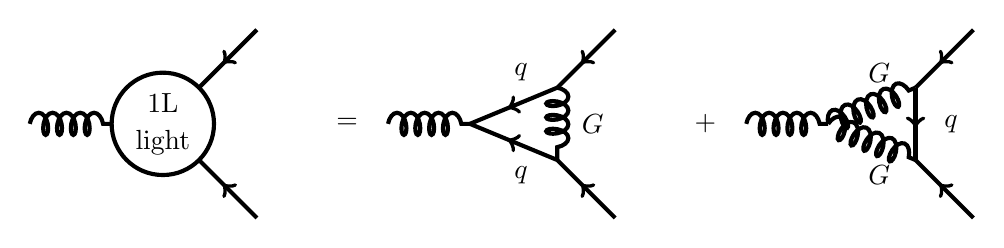
\begin{tikzpicture}[line width=1.5 pt, scale=1.3]
	\draw[gluon](180:1.3)--(180:0.5);
	\draw[fermionnoarrow] (-0.5,0) arc (180:0:.5);
	\draw[fermionnoarrow] (0.5,0) arc (0:-180:.5);	
	\node at (0,0.2) {1L};
	\node at (0,-0.18) {light};
	\draw[fermionbar](45:0.5)--(45:1.3);
	\draw[fermionbar](-45:0.5)--(-45:1.3);
	\node at (1.8,0) {=};
\begin{scope}[shift={(3.5,0)}]
	\draw[gluon](180:1.3)--(180:0.5);
	\draw[fermionbar](180:0.5)--(45:0.5);
	\node at (0,0.5) {$q$};
	\draw[fermionbar](180:0.5)--(-45:0.5);
	\node at (0,-0.5) {$q$};
	\draw[gluon](45:0.5)--(-45:0.5);
	\node at (0.7,0) {$G$};
	\draw[fermionbar](45:0.5)--(45:1.3);
	\draw[fermionbar](-45:0.5)--(-45:1.3);
	\node at (1.8,0) {+};
\end{scope}
\begin{scope}[shift={(7,0)}]
	\draw[gluon](180:1.3)--(180:0.5);
	\draw[gluon](180:0.5)--(45:0.5);
	\node at (0,0.5) {$G$};
	\draw[gluon](180:0.5)--(-45:0.5);
	\node at (0,-0.5) {$G$};
	\draw[fermion](45:0.5)--(-45:0.5);
	\node at (0.7,0) {$q$};
	\draw[fermionbar](45:0.5)--(45:1.3);
	\draw[fermionbar](-45:0.5)--(-45:1.3);
\end{scope}
\end{tikzpicture}
\caption{contribution from light particles to the $q\overline{q}G$ vertex correction}\label{fig:GaugeCouplingCorrection}
\end{center}
\end{figure}
\begin{align}
i\Gamma^{\mathrm{1L,light}}_{q_i \overline{q}_j G_\mu^a}|_{\mathrm{UV-div}} &= -i g_s T^a_{ij} \gamma^\mu \frac{g_s^2}{16\pi^2 \epsilon_{\mathrm{UV}}} \left[ \left(C(F) -\frac{C(A)}{2}\right) + \frac{3}{2} C(A) \right]
\end{align}
\begin{figure}[!htbp]
\begin{center}
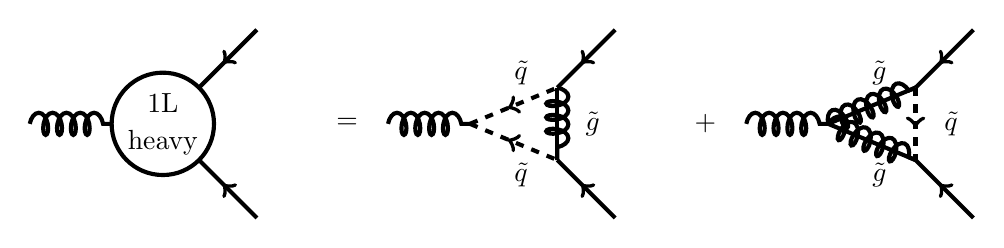
\begin{tikzpicture}[line width=1.5 pt, scale=1.3]
	\draw[gluon](180:1.3)--(180:0.5);
	\draw[fermionnoarrow] (-0.5,0) arc (180:0:.5);
	\draw[fermionnoarrow] (0.5,0) arc (0:-180:.5);	
	\node at (0,0.2) {1L};
	\node at (0,-0.18) {heavy};
	\draw[fermionbar](45:0.5)--(45:1.3);
	\draw[fermionbar](-45:0.5)--(-45:1.3);
	\node at (1.8,0) {=};
\begin{scope}[shift={(3.5,0)}]
	\draw[gluon](180:1.3)--(180:0.5);
	\draw[scalarbar](180:0.5)--(45:0.5);
	\node at (0,0.5) {$\tilde{q}$};
	\draw[scalarbar](180:0.5)--(-45:0.5);
	\node at (0,-0.5) {$\tilde{q}$};
	\draw[gluon](45:0.5)--(-45:0.5);
	\draw[fermionnoarrow](45:0.5)--(-45:0.5);
	\node at (0.7,0) {$\tilde{g}$};
	\draw[fermionbar](45:0.5)--(45:1.3);
	\draw[fermionbar](-45:0.5)--(-45:1.3);
	\node at (1.8,0) {+};
\end{scope}
\begin{scope}[shift={(7,0)}]
	\draw[gluon](180:1.3)--(180:0.5);
	\draw[gluon](180:0.5)--(45:0.5);
	\draw[fermionnoarrow](180:0.5)--(45:0.5);
	\node at (0,0.5) {$\tilde{g}$};
	\draw[gluon](180:0.5)--(-45:0.5);
	\draw[fermionnoarrow](180:0.5)--(-45:0.5);
	\node at (0,-0.5) {$\tilde{g}$};
	\draw[scalar](45:0.5)--(-45:0.5);
	\node at (0.7,0) {$\tilde{q}$};
	\draw[fermionbar](45:0.5)--(45:1.3);
	\draw[fermionbar](-45:0.5)--(-45:1.3);
\end{scope}
\end{tikzpicture}
\caption{contribution from heavy particles to the $q\overline{q}G$ vertex correction}
\end{center}
\end{figure}
\begin{align}
i\Gamma^{\mathrm{1L,heavy}}_{q_i \overline{q}_j G_\mu^a}|_{\mathrm{UV-div,\mu-dep}} = -i g_s T^a_{ij} \gamma^\mu \frac{g_s^2}{16\pi^2} &\left[ \left(C(F) -\frac{C(A)}{2}\right) \left( \frac{1}{\epsilon_{\mathrm{UV}}} - \ln \frac{m_{\tilde{g}}^2}{\mu^2} \right) \right.\nonumber\\
&+ \left.\frac{1}{2} C(A)\left( \frac{1}{\epsilon_{\mathrm{UV}}} - \ln \frac{m_{\tilde{g}}^2}{\mu^2} \right) \right]
\end{align}
The sum of the 1-loop corrections and the counterterm should be set to zero:
\begin{align}
i\Gamma^{\mathrm{1L,light}}_{q_i \overline{q}_j G_\mu^a}|_{\mathrm{UV-div}} + i\Gamma^{\mathrm{1L,heavy}}_{q_i \overline{q}_j G_\mu^a}|_{\mathrm{UV-div,\mu-dep}} + \left[ -ig_s T^a_{ij}\gamma^\mu\left( \frac{\delta g_s}{g_s} + \delta Z_q^{\mathrm{aux}} + \frac{\delta Z_G^{\mathrm{aux}}}{2} \right)\right] = 0.
\end{align}
Finally one can read off the $\frac{\delta g_s}{g_s}$
\begin{align}
\frac{\delta g_s}{g_s} &= \frac{g_s^2}{16\pi^2} \left[ \left( \frac{2}{3}T(F)(n_f-1) - \frac{11}{6}C(A) \right) \frac{1}{\epsilon_{\mathrm{UV}}} + \left( \frac{5}{6}C(A) + \frac{2}{3}T(F) + \frac{1}{3}T(F)n_f \right)\frac{1}{\epsilon_{\mathrm{UV}}}  \right.\nonumber\\
&- \frac{2}{3} C(A) \ln \frac{m_{\tilde{g}}^2}{\mu^2} - \frac{1}{3}T(F)n_f \ln \frac{m_{\tilde{q}}^2}{\mu^2} - \frac{2}{3}T(F) \ln \frac{m_t^2}{\mu^2}-\frac{1}{12} C(A) \left( \ln \frac{m_{\phi^0}^2}{\mu^2} + \ln \frac{m_{\sigma^0}^2}{\mu^2} \right)\label{eq:deltaGs}
\end{align}

\subsubsection{The Beta Function}
The beta function describes the dependence of the gauge coupling $g_s$ upon the energy scale $\mu$.\\
Writing down the action of a theory in $D$ dimensions one needs to introduce an energy scale $\mu$ in order to keep the action dimensionless. But $\mu$ is no physical parameter and can be absorped into the fields and parameters. To this end one defines
\begin{align}
g_{sB} = \mu^\epsilon g_s \left( 1 + \frac{\delta g_s}{g_s} \right)
\end{align}
which must not depend upon the unphysical scale $\mu$, ergo
\begin{align}
0 = \frac{\mathrm{d}g_{sB}}{\mathrm{d}\ln\mu} = \frac{\partial g_{sB}}{\partial \ln\mu} + \beta \frac{\partial g_{sB}}{\partial g_s}\label{eq:beta_func}
\end{align}
where the definition of the beta function $\frac{\partial g_s}{\partial\ln\mu}$ has been inserted. Equation \ref{eq:beta_func} serves to calculate $\beta(g_s,\epsilon)$.  By equating coefficients and using the shortcuts
\begin{align*}
\frac{\beta_0^L}{2} &= \frac{2}{3}T(F)(n_f-1) - \frac{11}{6}C(A)\\
\frac{\beta_0^H}{2} &= \frac{5}{6}C(A) + \frac{2}{3}T(F) + \frac{1}{3}T(F)n_f\\
L &= - \frac{2}{3} C(A) \ln \frac{m_{\tilde{g}}^2}{\mu^2} - \frac{1}{3}T(F)n_f \ln \frac{m_{\tilde{q}}^2}{\mu^2} - \frac{2}{3}T(F) \ln \frac{m_t^2}{\mu^2}-\frac{1}{12} C(A) \left( \ln \frac{m_{\phi^0}^2}{\mu^2} + \ln \frac{m_{\sigma^0}^2}{\mu^2} \right)
\end{align*}
so that 
\begin{align}
\frac{\delta g_s}{g_s} = \frac{g_s^2}{16\pi^2}\left( \frac{\beta^L_0}{2\epsilon_{\mathrm{UV}}} + \frac{\beta^H_0}{2\epsilon_{\mathrm{UV}}} + L \right)
\end{align}
one finds
\begin{align}
\beta(g_s,\epsilon) &= -\epsilon g_s \left( 1 + \frac{g_s^2}{16\pi^2} L \right) + \beta(g_s) + \mathcal{O}(\mathrm{2-loop})\\
\beta(g_s) &= \frac{g_s^3}{16\pi^2} \beta_0^L + \mathcal{O}(\mathrm{2-loop}).
\end{align}
This is the beta function from QCD first found by [Gross, Politzer, Wil]


\subsection{Supersymmetry Restoring Counterterm}
As already discussed in section \ref{sec:RegSchemeDep} care is required in terms of supersymmetry restoring when renormalizing  the gauge coupling $g_s$ and the Yukawa coupling $\hat{g}_s$. In doing so one needs the already calculated supersymmetry restoring counterterms of the quark, squark and gluino from \ref{eq:QuarkSC}, \ref{eq:SquarkSC} and \ref{eq:GluinoSC}
as well as the supersymmetry restoring counterterm of the gluon.
\subsubsection*{The Gluon Self-Energy Revisited}
The only regularization dependence of the gluon self-energy arises from the gluon loop, i.e. the last diagram in figure \ref{fig:lightGluonSelfEnergy}. With the definition of $\Gamma^{\mathrm{(1),ct,restore}}_{\mathrm{DREG}}$ in \ref{eq:GammaCtRestore} one obtains
\begin{align}
i\Gamma^{\mathrm{(1),ct,restore}}_{\mathrm{DREG},G_\mu^a G_\nu^b} = -i\frac{1}{3} C(A) \frac{g_s^2}{16\pi^2}(p^2 g^{\mu\nu}-p^\mu p^\nu)\delta_{ab}
\end{align}
which translates to the transition counterterm
\begin{align}
\delta Z^{\mathrm{trans}}_G = \frac{C(A)}{3}\frac{g_s^2}{16\pi^2}.
\end{align}

\subsubsection*{The $q\overline{q}G$ Vertex Correction Revisited}
The supersymmetry restoring contributions to the gauge coupling correction are shown in figure \ref{fig:GaugeCouplingCorrection} and evaluate to
\begin{align}
i\Gamma^{\mathrm{(1),ct,restore}}_{\mathrm{DREG}, q_i\overline{q}_jG_\mu^a} &= -ig_s T^a_{ij} \gamma^\mu \frac{g_s^2}{16\pi^2}\left[ \left( C(F) - \frac{C(A)}{2} \right) + \frac{C(A)}{2} \right]\\
&= -ig_s T^a_{ij} \gamma^\mu \left[ \frac{\delta g_s^{\mathrm{trans}}}{g_s} + \delta Z^{\mathrm{trans}}_q + \frac{\delta Z^{\mathrm{trans}}_G}{2} \right]
\end{align}
where in the second line the equation with the supersymmetry restoring counterterms has been performed. This yields
\begin{align}
\frac{\delta g_s^{\mathrm{trans}}}{g_s} = -\frac{C(A)}{6} \frac{g_s^2}{16\pi^2}.
\end{align}

\subsubsection*{The $q\tilde{q}^\dagger\tilde{g}$ Vertex Correction}
The supersymmetry restoring corrections to the Yukawa coupling origin from the below diagram 
\begin{figure}[!htbp]
\begin{center}
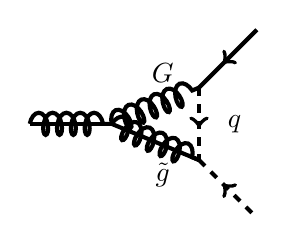
\begin{tikzpicture}[line width=1.5 pt, scale=1.3]
	\draw[gluon](180:1.3)--(180:0.5);
	\draw[fermionnoarrow](180:1.3)--(180:0.5);
	\draw[gluon](180:0.5)--(45:0.5);
	\node at (0,0.5) {$G$};
	\draw[fermionnoarrow](180:0.5)--(-45:0.5);
	\draw[gluon](180:0.5)--(-45:0.5);
	\node at (0,-0.5) {$\tilde{g}$};
	\draw[scalar](45:0.5)--(-45:0.5);
	\node at (0.7,0) {$q$};
	\draw[fermionbar](45:0.5)--(45:1.3);
	\draw[scalarbar](-45:0.5)--(-45:1.3);
\end{tikzpicture}
\caption{diagram of the supersymmetry restoring correction of  the $q\tilde{q}\tilde{g}$ vertex}
\end{center}
\end{figure}
The supersymmetry restoring part is
\begin{align}
i\Gamma^{\mathrm{(1),ct,restore}}_{\mathrm{DREG}, q_i\tilde{q}_j\tilde{g}^a} &= -ig_s \sqrt{2} P_L T^a_{ij}  \frac{g_s^2}{16\pi^2}C(A)\\
&= -ig_s \sqrt{2} P_L T^a_{ij}  \left[ \frac{\delta \hat{g}_s^{\mathrm{trans}}}{g_s} + \frac{\delta Z^{\mathrm{trans}}_q + \delta Z^{\mathrm{trans}}_{\tilde{q}} + \delta Z^{\mathrm{trans}}_{\tilde{g}}}{2} \right].
\end{align}
The supersymmetry restoring part of the Yukawa renormalization constants is therefore
\begin{align}
\frac{\delta \hat{g}_s^{\mathrm{trans}}}{g_s} = -\frac{C(F)-C(A)}{2} \frac{g_s^2}{16\pi^2}.
\end{align}
As a consequence of the two different supersymmetry restoring parts of the coupling renormalization constants an additional renormalization constant $\delta g_s^{\mathrm{restore}}$ needs to be introduced. As described in section \label{sec:RegSchemeDep} it is given by
\begin{align}
\frac{\delta g_s^{\mathrm{restore}}}{g_s} = \frac{\delta \hat{g}_s^{\mathrm{trans}}}{g_s} -\frac{\delta g_s^{\mathrm{trans}}}{g_s} = \frac{g_s^2}{16\pi^2}\left( \frac{2C(A)}{3} - \frac{C(F)}{2} \right).
\end{align}
In short this means that the gauge coupling $g_s$ is renormalized with $\delta g_s$ given in \ref{eq:deltaGs} and the Yukawa coupling $\hat{g}_s$ is renormilzed with $\delta \hat{g}_s = \delta g_s + \delta g_s^{\mathrm{restore}}$.\\
The finite correction $g_s^{\mathrm{restore}}$ is the same as in supersymmetric QCD which should not surprise too much as all its contributions origin from loops with gluons. So there are no new contributions in RSQCD with respect to SQCD. 


\subsection{$\overline{\mathrm{MS}}$ - Renormalization}
To check for UV-finiteness it might prove useful to summarize the UV-divergent part of all renormalization constants. In order to obtain these the Passarino-Veltman integrals need to be substituted by their $\frac{1}{\epsilon}$ coefficient. These  had been taken from \cite{Denner} and checked with \texttt{FeynArts} and \texttt{FormCalc} \cite{Hahn:2000}, \cite{Nejad2013}, \cite{Hahn:2000}.
\newpage
\section{Squark Production at One-Loop}


\subsection{The LSZ Theorem}\label{sec:LSZ}
The LSZ theorem\cite{Lehmann:1954rq} or LSZ reduction formula prescribes how to obtain the S-matrix element, i.e. a physical observable, from the time ordered correlation function of the respective field operators. The time ordered correlation function of fields in an interacting theory can be calculated perturbatively with the aid of the Gell-Mann and Low theorem and the Wick theorem. \\
Considering a physical process with kinematics $\vec{k}_1 \hdots \vec{k}_n \to \vec{p}_1 \hdots \vec{p}_m$ and taking for the sake of simplicity only one scalar field $\phi$ the Fourier transform of the time ordered product of a correlation function is related to the corresponding S-matrix element like\footnote{In this subsection the $\sim$ indicates that the poles on either side are the same provided that all momenta are close to their mass shell, i.e. $p_i^0 \to E_{\vec{p}_i}$ and $k_j^0 \to E_{\vec{k}_j}$.}
\begin{align}
\prod_{i=1}^n \int \mathrm{d}x_i\ \mathrm{e}^{ip_i x_i} \prod_{j=1}^m \int \mathrm{d}y_j\ \mathrm{e}^{ik_j y_j} \left\langle \Omega | \mathcal{T} \left[ \phi(x_1) \hdots \phi(x_n) \phi(y_1) \hdots \phi(y_m) \right] | \Omega\right\rangle \nonumber\\
\sim \prod_{i=1}^n \frac{i\sqrt{Z}}{p_i^2 - m^2 + i\epsilon} \prod_{j=1}^m \frac{i\sqrt{Z}}{k_j^2 - m^2 + i\epsilon} \left\langle \left.\left.\vec{p}_1 \hdots \vec{p}_n \right| S \right| \vec{k}_1 \hdots \vec{k}_m \right\rangle .\label{eq:LSZ}
\end{align}
Here $\mathcal{T}$ denotes the time ordering operator, $\left.| \Omega \right\rangle$ is the ground state of the interacting theory and $\sqrt{Z}$ is the residue of the single particle pole in the two-point function 
\begin{align}
\int \mathrm{d}x\ \mathrm{e}^{ip x} \left\langle \Omega | \mathcal{T} \left[ \phi(x) \phi(0) \right] | \Omega\right\rangle &= \frac{i}{p^2-m_0^2} + \frac{i}{p^2-m_0^2} \left(\frac{i\Sigma(p^2)}{p^2-m_0^2}\right) + \frac{i}{p^2-m_0^2} \left(\frac{\Sigma(p^2)}{p^2-m_0^2}\right)^2 + \hdots\nonumber\\
&= \frac{i}{p^2 - m_0^2 - \Sigma(p^2)}.\label{eq:propagator}
\end{align}
\begin{figure}[!htbp]
\begin{center}
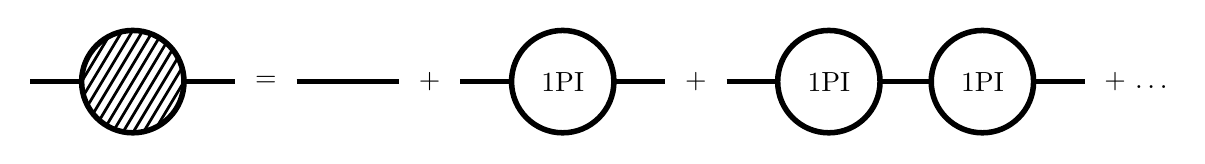
\begin{tikzpicture}[line width=2.0 pt, scale=1.3]
	\draw[fermionnoarrow](180:1)--(180:0.5);	
	\draw (0,0) circle (.5cm);
		\begin{scope}
	    	\clip (0,0) circle (.5cm);
	    	\foreach \x in {-1.0,-0.9,...,1.0}
        \draw[line width=1 pt] (\x,-.5) -- (\x+.6,.5);
	  	\end{scope}
	\draw[fermionnoarrow](0:0.5)--(0:1);
	\node at (1.3,0) {=};
	\draw[fermionnoarrow](0:1.6)--(0:2.6);
	\node at (2.9,0) {+};
    \draw[fermionnoarrow](0:3.2)--(0:3.7);	
	\draw (4.2,0) circle (.5cm);
	\node at (4.2,0) {1PI};
	\draw[fermionnoarrow](0:4.7)--(0:5.2);
	\node at (5.5,0) {+};	
	\draw[fermionnoarrow](0:5.8)--(0:6.3);	
	\draw (6.8,0) circle (.5cm);
	\node at (6.8,0) {1PI};
	\draw[fermionnoarrow](0:7.3)--(0:7.8);
	\draw (8.3,0) circle (.5cm);
	\node at (8.3,0) {1PI};
	\draw[fermionnoarrow](0:8.8)--(0:9.3);
	\node at (9.8,0) {+ $\hdots$};
\end{tikzpicture}
\caption{Diagrammatic figure of the two-point function of a scalar field: The propagator in an interaction theory can be calculated in a perturbation series in the coupling constant.}\label{fig:fullpropagator}
\end{center}
\end{figure}
The parameter $m_0$ is the tree-level mass and the quantity $-i \Sigma(p^2)$ denotes the sum of all one-particle-irreducible contributions to the particle's self-energy. From eq. \eqref{eq:propagator} one can read off the physical mass $m^2$ of the particle which is associated with the field $\phi$. It is determined as the value of $p^2$ where the propagator has a pole, i.e. 
\begin{align}
\left[ p^2 - m_0^2 - \Sigma(p^2)\right]_{p^2 = m^2} = 0
\end{align}
Close to the pole the denominator of eq. \eqref{eq:propagator} can by expanded like
\begin{align}
p^2 - m_0^2 - \Sigma(p^2) = (p^2 - m^2)\left( 1 - \frac{\partial \Sigma(p^2)}{\partial p^2} \right)_{p^2 = m^2} + \mathcal{O}((p^2 - m^2)^2).
\end{align}
The residue of the propagator can therefore be written as 
\begin{align}
Z = \left( 1 - \frac{\partial \Sigma(p^2)}{\partial p^2} \right)_{p^2 = m^2}^{-1}.
\end{align}
Now considers the full $(n+m)$-point function in scalar theory. One can decompose it into an amputated $(n+m)$-point function and "full" propagators like written in eq. \eqref{eq:propagator} and depicted in fig. \ref{fig:fullpropagator}.
\begin{figure}[!htbp]
\begin{center}
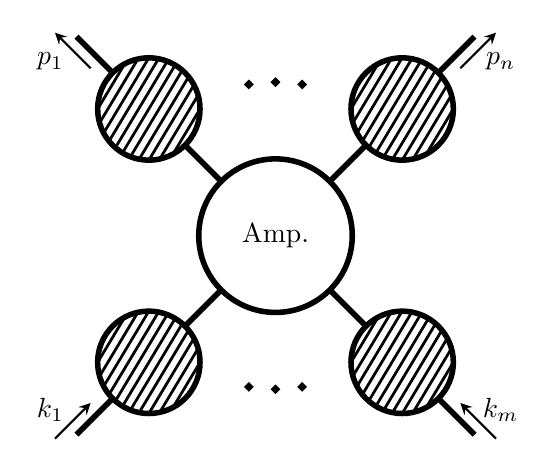
\begin{tikzpicture}[line width=2.0 pt, scale=1.3, arrow/.style={thick,->,shorten >=2pt,shorten <=2pt,>=stealth}]
	\draw (0,0) circle (.75);
	\node at (0,0) {Amp.};
	\draw (45:0.75)--(45:1.25);
	\draw (45:1.75) circle (.5);
		\begin{scope}[shift={(45:1.75)}]
	    	\clip (0,0) circle (.5cm);
	    	\foreach \x in {-1.0,-0.9,...,1.0}
        \draw[line width=1 pt] (\x,-.5) -- (\x+.6,.5);
	  	\end{scope}
	\draw (45:2.25)--(45:2.75);
	\draw[arrow] (1.768,1.597)--(2.192,2.021);
	\node at (2.2,1.7){$p_n$};

	\draw (135:0.75)--(135:1.25);
	\draw (135:1.75) circle (.5);
		\begin{scope}[shift={(135:1.75)}]
	    	\clip (0,0) circle (.5cm);
	    	\foreach \x in {-1.0,-0.9,...,1.0}
        \draw[line width=1 pt] (\x,-.5) -- (\x+.6,.5);
	  	\end{scope}
	\draw (135:2.25)--(135:2.75);
	\draw[arrow] (-1.768,1.597)--(-2.192,2.021);
	\node at (-2.2,1.7){$p_1$};	
	
	\draw (225:0.75)--(225:1.25);
	\draw (225:1.75) circle (.5);
		\begin{scope}[shift={(225:1.75)}]
	    	\clip (0,0) circle (.5cm);
	    	\foreach \x in {-1.0,-0.9,...,1.0}
        \draw[line width=1 pt] (\x,-.5) -- (\x+.6,.5);
	  	\end{scope}
	\draw (225:2.25)--(225:2.75);
	\draw[arrow] (-2.192,-2.021)--(-1.768,-1.597);
	\node at (-2.2,-1.7){$k_1$};	
	
	\draw (315:0.75)--(315:1.25);
	\draw (315:1.75) circle (.5);
		\begin{scope}[shift={(315:1.75)}]
	    	\clip (0,0) circle (.5cm);
	    	\foreach \x in {-1.0,-0.9,...,1.0}
        \draw[line width=1 pt] (\x,-.5) -- (\x+.6,.5);
	  	\end{scope}
	\draw (315:2.25)--(315:2.75);
	\draw[arrow] (2.192,-2.021)--(1.768,-1.597);
	\node at (2.2,-1.7){$k_m$};
	
	\draw[fill=black] (80:1.5) circle (.01);
	\draw[fill=black] (90:1.5) circle (.01);
	\draw[fill=black] (100:1.5) circle (.01);
	\draw[fill=black] (-80:1.5) circle (.01);
	\draw[fill=black] (-90:1.5) circle (.01);
	\draw[fill=black] (-100:1.5) circle (.01);
\end{tikzpicture}
\caption{Diagrammatic figure of a "full" $(n+m)$-point function. Apart from the "full" propagators there is the "full" amputated $(n+m)$-point function}
\end{center}
\end{figure}\\
Inserting the expression
\begin{align}
\frac{i}{p^2 - m_0^2 - \Sigma(p^2)} \sim \frac{i Z}{p^2 - m^2}
\end{align}
for the full propagators one notices the same singularity as in eq. \eqref{eq:LSZ}. If one now compares the coefficients of these poles in eq. \eqref{eq:LSZ} one finds
\begin{figure}[!htbp]
\begin{center}
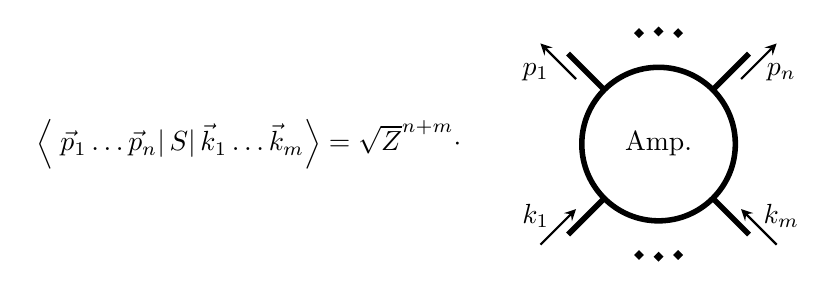
\begin{tikzpicture}[line width=2.0 pt, scale=1.3, arrow/.style={thick,->,shorten >=2pt,shorten <=2pt,>=stealth}]
	\node at (-4,0) {$\left\langle \left.\left.\vec{p}_1 \hdots \vec{p}_n \right| S \right| \vec{k}_1 \hdots \vec{k}_m \right\rangle =\sqrt{Z}^{n+m} \cdot$};
	\draw (0,0) circle (.75);
	\node at (0,0) {Amp.};

	\draw (45:0.75)--(45:1.25);
	\draw[arrow] (0.768,0.597)--(1.192,1.021);
	\node at (1.2,0.7){$p_n$};

	\draw (135:0.75)--(135:1.25);
	\draw[arrow] (-0.768,0.597)--(-1.192,1.021);
	\node at (-1.2,0.7){$p_1$};	
	
	\draw (225:0.75)--(225:1.25);
	\draw[arrow] (-1.192,-1.021)--(-0.768,-0.597);
	\node at (-1.2,-0.7){$k_1$};	
	
	\draw (315:0.75)--(315:1.25);
	\draw[arrow] (1.192,-1.021)--(0.768,-0.597);
	\node at (1.2,-0.7){$k_m$};
	
	\draw[fill=black] (80:1.1) circle (.01);
	\draw[fill=black] (90:1.1) circle (.01);
	\draw[fill=black] (100:1.1) circle (.01);
	\draw[fill=black] (-80:1.1) circle (.01);
	\draw[fill=black] (-90:1.1) circle (.01);
	\draw[fill=black] (-100:1.1) circle (.01);
\end{tikzpicture}
\end{center}
\end{figure}\\
Now it becomes visible why the renormalization in the on-shell scheme
\begin{align}
\left.\frac{\partial \Sigma(p^2)}{\partial p^2}\right|_{p^2 = m^2} \stackrel{!}{=} 0
\end{align}
introduces no further manipulation when turning from the correlation function to the S-matrix-element because $Z = 1$ in on-shell renormalization. Furthermore the on-shell condition for the mass renormalization
\begin{align}
\Sigma(p^2)|_{p^2 = m^2} = 0
\end{align}
means that the physical mass equals the tree level mass.

\subsection{The Squark Production Cross Section at Next-to-Leading Order}
The squark production cross section at next-to-leading order is composed out of three contributions. These are the Born or tree-level cross section, the virtual correction and the real correction. 
\begin{align}
\sigma^{\mathrm{NLO}} = \sigma^{\mathrm{B}} + \sigma^{\mathrm{V}} + \sigma^{\mathrm{R}}\label{eq:BVR}
\end{align}
All three contributions have to be calculated with next-to-leading parton density functions.\\
It has been checked that for multiple different and quite distinct choices of the parameters $m_{\tilde{q}}$ and $m_{\tilde{g}}$ the double as well as the single poles of the virtual and real correction cancel up to machine precision. As the real corrections have been calculated analytically it is possible to quote the double pole. With
\begin{align}
\sigma^{\mathrm{R}}_{\mathrm{double\ pole}} = -\sigma^{\mathrm{V}}_{\mathrm{double\ pole}} = C(F)\frac{\alpha_s}{\pi}\sigma^{\mathrm{B}} \frac{1}{\epsilon^2}
\end{align}
it has a very succinct form. \\
The setup of the calculation is summarized in fig. \ref{fig:CalcSetup}. Both the virtual and the Born matrix amplitude have been generated with the \texttt{Mathematica} package \texttt{FeynArts}. To this end a modelfile generated by the \texttt{Mathematica} package \texttt{SARAH} has been adjusted by hand to include counterterm Feynman rules and the definition of those counterterms. The matrix amplitudes have been processed further to the absolute squared matrix amplitudes by the \texttt{Mathematica} package \texttt{FormCalc} which have then been converted to \texttt{C++} and stored in an output file.\\
This output file is in turn invoked by a \texttt{C++} code which evaluates the scalar integrals of the absolute squared matrix amplitudes numerically by using the package \texttt{LoopTools} \cite{Hahn:1998}. Finally the phase space integration is performed by the integration routine "Cuhre" which is part of the \texttt{CUBA} library\cite{Hahn:2004fe}.\\
Comment on how real corrections are processed.\\
\begin{figure}[!htbp]
\begin{center}
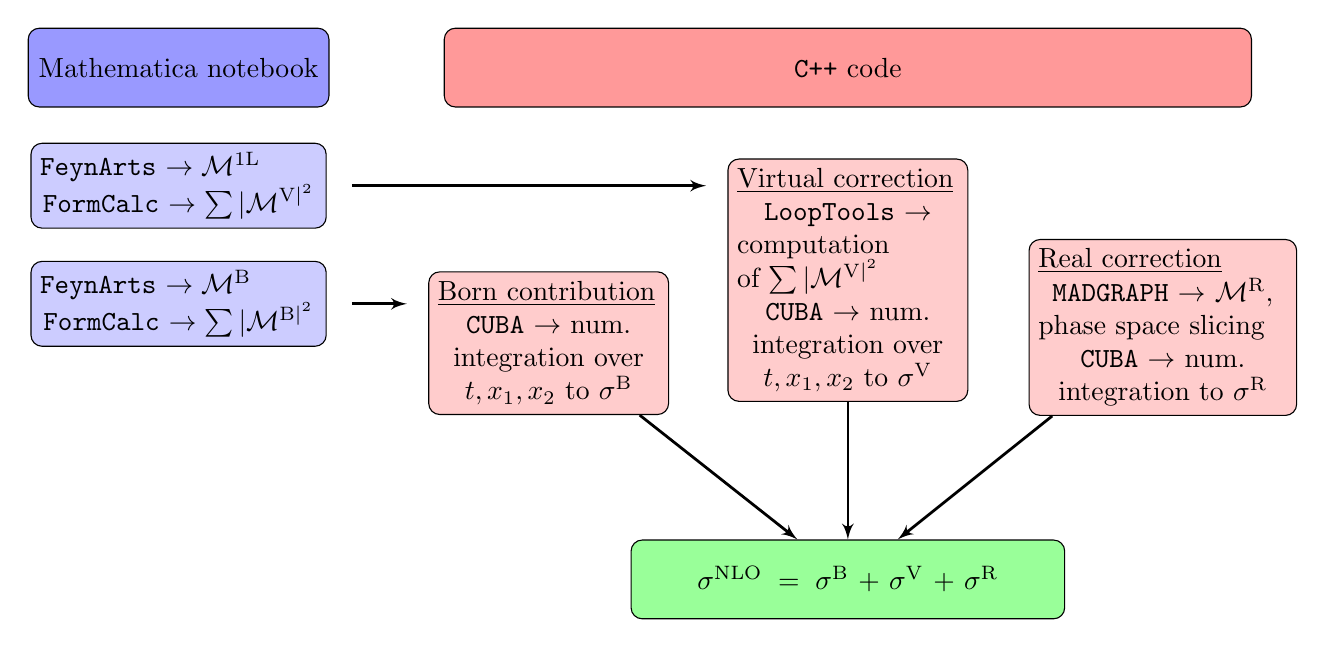
\begin{tikzpicture}
	\node [block4] at (-1,0) (Mathematica) {Mathematica notebook};
	\node [block1a] at (-1,-3) (notebookB) {\texttt{FeynArts} $\to \mathcal{M}^{\mathrm{B}}$ \newline \texttt{FormCalc} $\to \sum |\mathcal{M}^{\mathrm{B}|^2}$};	
	\node [block1a] at (-1,-1.5) (notebookV) {\texttt{FeynArts} $\to \mathcal{M}^{\mathrm{1L}}$ \newline \texttt{FormCalc} $\to \sum |\mathcal{M}^{\mathrm{V}|^2}$};
	\node [block5a] at (7.5,0) (C++) {\texttt{C++} code};
	\node [block5b] at (3.7,-3.5) (Born) {\underline{Born contribution} \newline \texttt{CUBA} $\to$ num. integration over $t, x_1, x_2$ to $\sigma^{\mathrm{B}}$};
	\node [block5b] at (7.5,-2.7) (Virt) {\underline{Virtual correction}\newline \texttt{LoopTools} $\to$ computation \newline of $ \sum |\mathcal{M}^{\mathrm{V}|^2}$ \newline \texttt{CUBA} $\to$ num. integration over $t, x_1, x_2$ to $\sigma^{\mathrm{V}}$};
	\node [block5c] at (11.5,-3.3) (Real) {\underline{Real correction}\newline \texttt{MADGRAPH} $\to$ $\mathcal{M}^{\mathrm{R}}$, phase space slicing\newline \texttt{CUBA} $\to$ num. integration to $\sigma^{\mathrm{R}}$};
	\path [line, line width = 1] (1.2,-3) -- (1.9,-3);
	\path [line, line width = 1] (1.2,-1.5) -- (5.7,-1.5);
	\node [block6a] at (7.5,-6.5) (Sigma) {$\sigma^{\mathrm{NLO}} = \sigma^{\mathrm{B}} + \sigma^{\mathrm{V}} + \sigma^{\mathrm{R}}$};
	\path [line, line width = 1] (Born) -- (Sigma);
	\path [line, line width = 1] (Virt) -- (Sigma);
	\path [line, line width = 1] (Real) -- (Sigma);
\end{tikzpicture}
\caption{This scheme illustrates the setup of the computation of the next-to-leading order cross section. The absolute squared matrix amplitudes of the Born or tree-level contribution and the virtual correction are generated by \texttt{Mathematica} packages and imported into a \texttt{C++} code. Loop integrals are evaluated numerically using \texttt{Looptools}. For all three contributions the \texttt{CUBA}-library was used for the phase space and $x_1$ and $x_2$ integration to arrive at the cross sections $\sigma^{\mathrm{B}}$, $\sigma^{\mathrm{V}}$ and $\sigma^{\mathrm{V}}$.  The real corrections have been calculated by Wojciech Kotlarski, another member of the group.}\label{fig:CalcSetup}
\end{center}
\end{figure}

\subsubsection{Remark on Prefactors in the Calculation}
For the discussion of results it will not been distinguished between virtual and real corrections. This is because they have not been separated strictly in the calculation: As already discussed both $\sigma^{\mathrm{V}}$ and $\sigma^{\mathrm{R}}$ are divergent, i.e. there are poles of the form $\frac{1}{\epsilon}$ and $\frac{1}{\epsilon^2}$. But these pole cancel completely. On the other hand there are also prefactors from the phase space integral and the loop integral, with can be expanded in a power series in $\epsilon$. In short, the virtual and real correction to the cross section can be expressed with some coefficients $A - E$, which are functions of the parameters $m_{\tilde{g}}$ and $m_{\tilde{q}}$, in the following way
\begin{align}
\sigma^{\mathrm{V}} &= \left( 1 + (A^{\mathrm{V}} + P_1)\epsilon + (B^{\mathrm{V}} + P_2)\epsilon^2 + \mathcal{O}(\epsilon^3) \right)\left( C^{\mathrm{V}} - \frac{D}{\epsilon} - \frac{E}{\epsilon^2} \right),\\
\sigma^{\mathrm{R}} &= \left( 1 + (A^{\mathrm{R}} + P_1)\epsilon + (B^{\mathrm{R}} + P_2)\epsilon^2 + \mathcal{O}(\epsilon^3) \right)\left( C^{\mathrm{R}} + \frac{D}{\epsilon} + \frac{E}{\epsilon^2} \right).\label{eq:prefactoredecomp}
\end{align}
Here, the coefficients $A$, $B$ and $C$ are in general distinct in the virtual and real part, but $D$ and $E$ are the same as the poles of both contributions cancel exactly.\\
Now some of the prefactors, namely $P_1$ and $P_2$, are the same in both contributions. Just keeping them like in eq. \eqref{eq:prefactoredecomp} would slow the computation of the real part down by a factor 5 because this part of the calculation is done analytically. Therefore a speed-up has been achieved by discarding the common prefactors at the cost of loosing track about the origin of the next-to-leading order correction.\\
A common prefactor comes from the two-body phase space integral in eq. \eqref{eq:diffsigma}
\begin{align}
\frac{(4\pi)^\epsilon}{\Gamma(1-\epsilon)}\left( \frac{tu - m_{\tilde{q}}^4}{\mu^2 s} \right)^{-\epsilon} = 1 &+ \epsilon\left( \ln 4\pi -\gamma_E - \ln \frac{tu - m_{\tilde{q}}^4}{\mu^2 s} \right) 
+ \epsilon^2\left( \frac{1}{2}\left( \ln 4\pi - \ln \frac{tu - m_{\tilde{q}}^4}{\mu^2 s} \right)^2 \right.\nonumber\\
&+ \left.\frac{\gamma_E^2}{2} - \frac{\pi^2}{12} - \gamma_E\left( \ln 4\pi - \ln \frac{tu - m_{\tilde{q}}^4}{\mu^2 s} \right) \right) + \mathcal{O}(\epsilon^3).\label{eq:PhasePrefactor}
\end{align}
In addition the prefactor of a loop integral defined in \texttt{LoopTools} differs from the one usually, and therefore also here, used. The \texttt{LoopTools} definition\cite{LoopToolsManual} of a loop integral is 
\begin{align}
T^N_{\mu_1\hdots\mu_P} = \frac{\mu^{4-D}}{i\pi^{\frac{D}{2}}r_\Gamma}\int\mathrm{d}^Dq\frac{q_{\mu_1} \hdots q_{\mu_P}}{[q^2-m_1^2] [(q+p_1)^2-m_2^2] \hdots [(q+p_1+ \hdots +p_{N-1})^2-m_N^2]}\label{eq:LoopToolsInt}
\end{align}
where $T^1$ is an $A$-integral, $T^2$ is an $B$-integral, etc. and $r_\Gamma = \frac{\Gamma(1-\epsilon)^2\Gamma(1+\epsilon)}{\Gamma(1-2\epsilon)}$, where $\Gamma(z)$ is the Gamma function. Comparing the prefactors of eq. \eqref{eq:LoopToolsInt} and eq.  \eqref{eq:LoopInt} one finds that one has to multiply the \texttt{LoopTools} output by
\begin{align}
r_\Gamma (4\pi)^\epsilon = 1 + \epsilon(\ln 4\pi -\gamma_E) + \epsilon^2\left( \frac{\gamma_E^2}{2} - \frac{\pi^2}{12} + \frac{\ln^2 4\pi}{2} - \gamma_E\ln 4\pi \right) + \mathcal{O}(\epsilon^3)\label{eq:LoopPrefactor}
\end{align}
in order to have the same prefactors as in eq. \eqref{eq:LoopInt}. The right hand side of eq. \eqref{eq:PhasePrefactor} and eq. \eqref{eq:LoopPrefactor} are the prefactors discarded in the computation. Instead the prefactor ??? has been included in the virtual correction.


\subsubsection{$K$-factors for Squark Production in the MRSSM}
A common way to describe next-to-leading order corrections is stating the $K$-factor, which is defined to be the ratio of the complete next-to-leading order cross section $\sigma^{\mathrm{NLO}}$, see eq. \eqref{eq:BVR} and the leading order cross section $\sigma^{\mathrm{LO}}$:
\begin{align}
K(X \to Y) = \frac{\sigma^{\mathrm{NLO}}(X \to Y)}{\sigma^{\mathrm{LO}}(X \to Y)}.
\end{align}
The process in question is described by $X \to Y$.
Figure \ref{fig:1LXsection_fixed_m} shows the $K$-factor for the production of up-squarks in the MRSSM for varying masses of both the squark ($m_{\tilde{g}} = \unit[2000]{GeV}$) and the gluino $m_{\tilde{q}} = \unit[1000]{GeV}$. The mass of the pseudoscalar has been fixed to $m_{\sigma} = \unit[5000]{GeV}$ in both plots. It can be seen that the  $K$-factor increases with increasing squark mass and decreases with increasing gluino mass. Note that the sum of virtual and real corrections gets negative for very light squarks. But this region of parameter space is already excluded phenomenologically.
\begin{figure}[!htpb]
\begin{center}
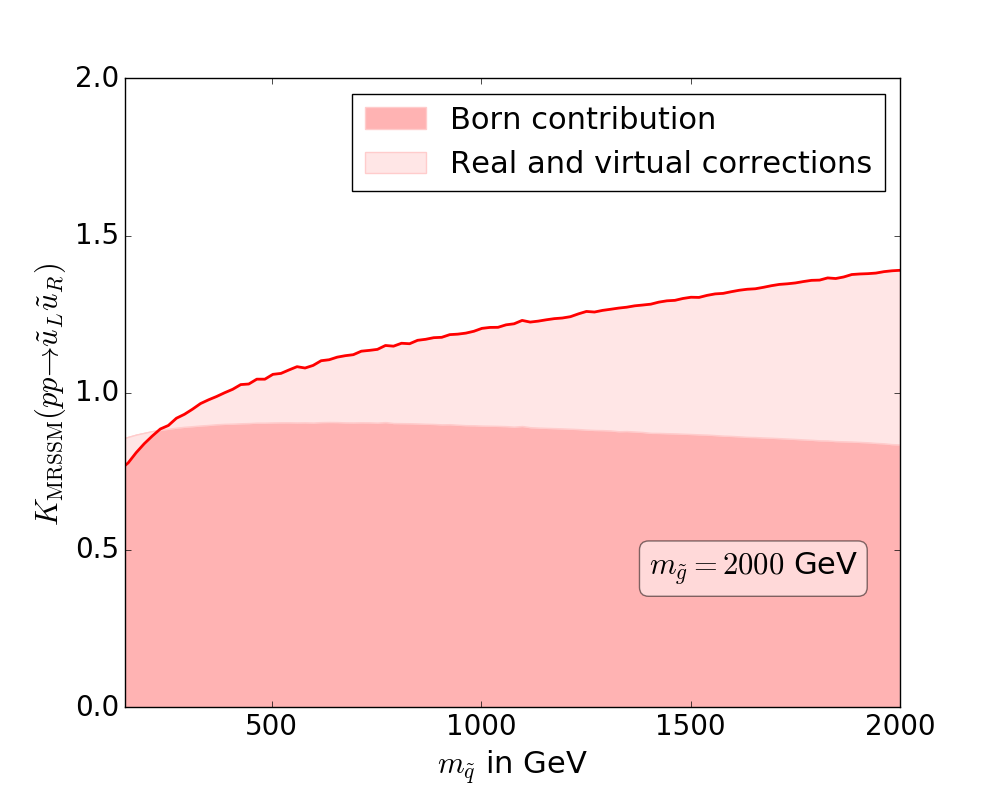
\includegraphics[scale=.5]{figures/MRSSM_uu_susu_Kfactors_msg=2000GeV.png}
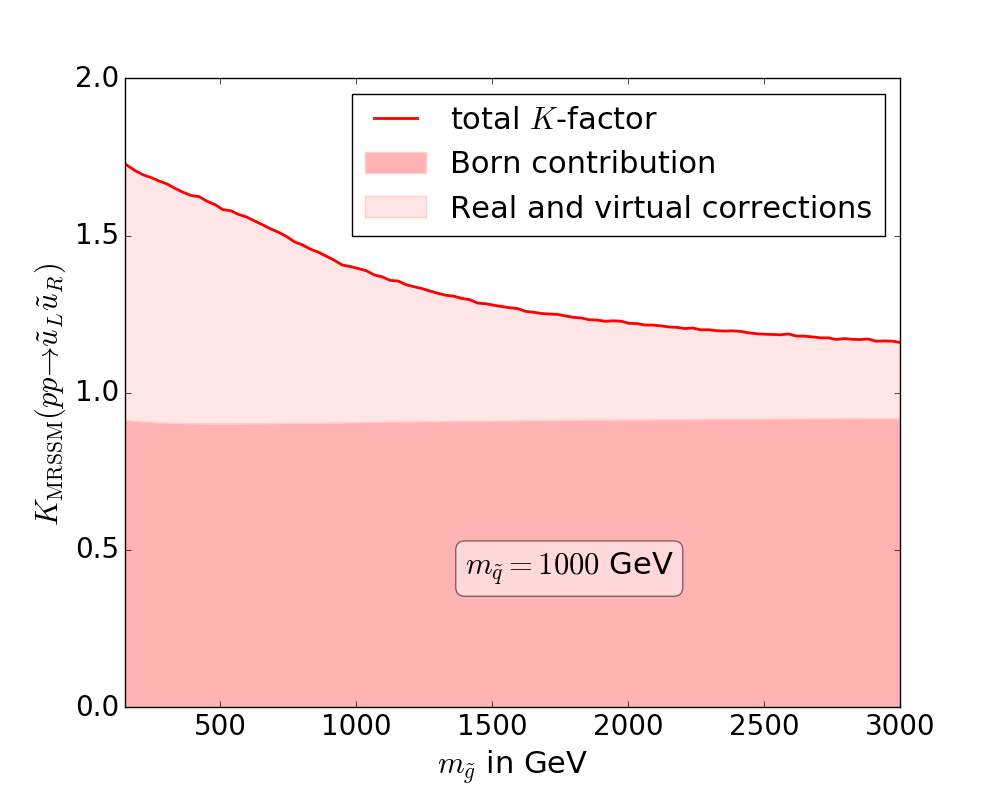
\includegraphics[scale=.5]{figures/MRSSM_uu_susu_Kfactors_msq=1000GeV.png}
\caption{Dependence of the $K$-factor for the process $uu \to \tilde{u}\tilde{u}$ on the squark mass $m_{\tilde{q}}$ for fixed $m_{\tilde{g}} = \unit[2000]{GeV}$ (top) and on the gluino mass $m_{\tilde{g}}$ for fixed $m_{\tilde{q}} = \unit[1000]{GeV}$ (bottom).}\label{fig:1LXsection_fixed_m}
\end{center}
\end{figure}
Calculate uncertainties for multiple points(pdf, scale, integration)


\subsection{The Cross Section in the Limit of Large Sgluon Masses}
The cross section for squark production does not exist in the limit of an infinitely large sgluon mass, instead it was found that it diverges logarithmically.\\
\begin{align}
\lim_{m_{\sigma}\to\infty} \sigma(qq \to \tilde{q}\tilde{q}) \sim \ln \frac{m_{\sigma}^2}{\mu^2}
\end{align}
This is actually expected as an effective field theory of the MRSSM where the sgluon is integrated out is no longer supersymmetric. This is because the sgluon is together with the octino part of a supermultiplet. Integrating out only the sgluon means that the octino misses its superpartner in the effective field theory. In this case the decoupling theorem \cite{Appelquist:1974tg} does no longer hold.\\
It is even possible to predict the  logarithmic scaling of $\sigma(qq \to \tilde{q}\tilde{q})$ quantitatively. The coefficient of the logarithm is proportional to the difference of the one-loop $\beta$ function coefficients of $g_s$ and $\hat{g}_s$ in the effective theory with the heavy particle integrated out, see eq. (4) in \cite{Cheng:1997sq}.
\begin{figure}[!htpb]
\begin{center}
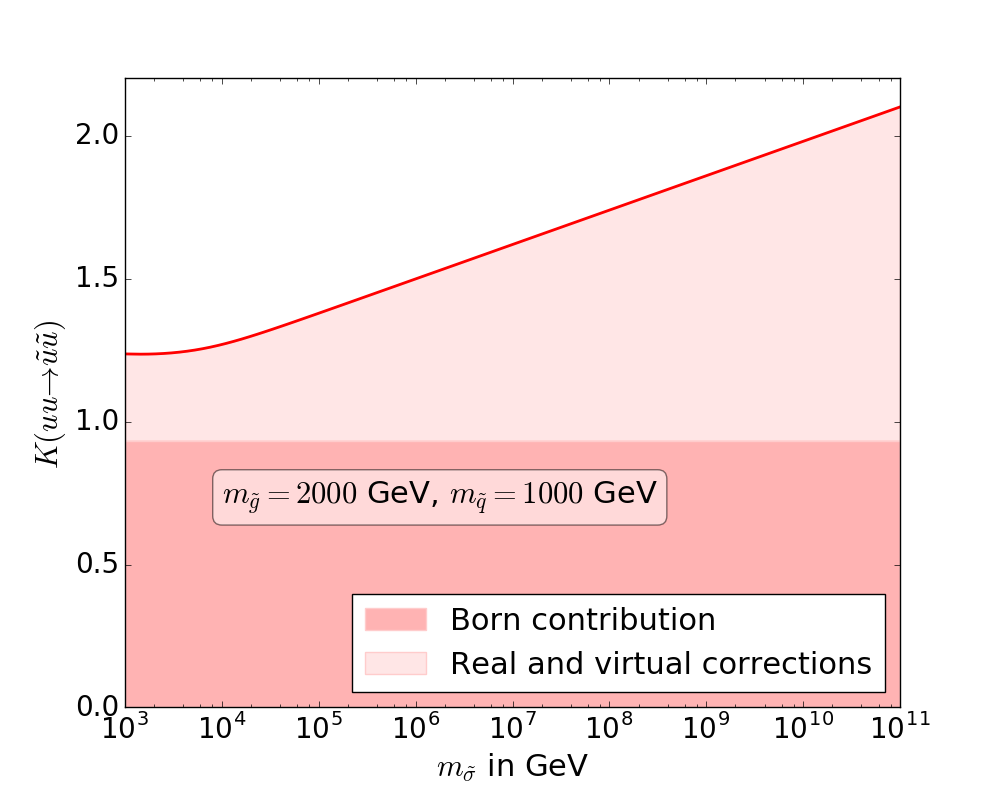
\includegraphics[scale=.5]{figures/MRSSM_uu_susu_Kfactors_msq=1000GeV_msg=2000GeV.png}
\caption{Dependence of the $K$-factor for the process $uu \to \tilde{u}\tilde{u}$ on the mass of the pseudoscalar sgluon. For $m_{\sigma} \approx \unit[10^5]{GeV}$ onwards want find a logarithmic scaling as predicted by \cite{Cheng:1997sq}.}
\end{center}
\end{figure}


\newpage
\section{Summary and Outlook}
\newpage
\section{Appendix}


\subsection{System of Units and Metric}
In this thesis the natural units are used, i.e. $c= \hbar (= k_B) = 1$. Furthermore the Minkowski metric is chosen to be
\begin{align}
g^{\mu\nu} = \mathrm{diag}(1, -1, -1, -1).
\end{align}


\subsection{Constants of the Color Algebra $SU(N)$}\label{sec:coloralgebra}
[Marina von Steinkirch]\\
Tha Casimir operator $C(R)\mathbbm{1}$ of a semi-simple Lie algebra in the irreducible representation $R$ is given by
\begin{align}
g^{ab} T^a(R)T^b(R) = C(R)\mathbbm{1} \label{eq:Casimir}
\end{align}
where $T^a(R)$ is the $a$-th generator of the matrix valued representation $R$, $g^{ab}$ is the metric of group, $C(R)$ is the Quadratic Casimir invariant of the representation $R$ and $\mathbbm{1}$ is the identity in the representation space.\\
Apart from $C(R)$ it is common to define the Dynkin-Index $T(R)$:
\begin{align}
\mathrm{Tr}\left[T^a(R)T^b(R)\right] = T(R)\delta^{ab}.
\end{align}
The two constants are connected by
\begin{align}
C(R) \cdot \mathrm{dim}(R) = T(R) \cdot \mathrm{dim}(G)
\end{align}
where $\mathrm{dim}(G)$ is the dimension of the group and $\mathrm{dim}(R)$ is the dimension of the irreducible representation $R$.\\
In the case of $SU(N)$ one has a diagonal metric $g^{ab} = \delta^{ab}$ and therefore \ref{eq:Casimir} turns to
\begin{align}
\sum_a (T^a(R))^2 = C(R)\mathbbm{1}_{\mathrm{dim}(R) \times \mathrm{dim}(R)}
\end{align}
and one can write down the following useful formulae for the fundamental representation $R=F$: $T^a_{ij} = \frac{\lambda^a_{ij}}{2}$ and the adjoint representation $R=A$: $(T^a_{ij})^{adj} = -if_{aij}$
\begin{align}
T^a_{ik} T^a_{kj} &= C(F)\mathbbm{1}_{ij} && \mbox{with}\ C(F) = \frac{N^2-1}{2N} = \frac{4}{3}\nonumber\\
f^{abc} f^{dbc} &= C(A)\delta^{ad} && \mbox{with}\ C(A) = N = 3\nonumber\\
\mathrm{Tr}\left[T^aT^b\right] &= T(F)\delta^{ab} && \mbox{with}\ T(F) = \frac{1}{2}\label{eq:DynkinIndex}
\end{align}
where $\lambda^a_{ij}$ are for $N_c = 3$ the Gell-Mann matrices and $f_{abc}$ are the structure constants of $SU(N_c)$.
%\begin{tabular}{c|c|c}
%Quadratic Casimir Invariant and $T(R)$ & $SU(N)_c$ & $SU(3)_c$\\
%\hline
%$C_2(3)$ & $\frac{N^2-1}{2N}$ & $\frac{4}{3}$\\
%$C_2(8)$ & $N$ & $3$\\
%$T(3)$ & $\frac{1}{2}$ & $\frac{1}{2}$ \\
%$T(8)$ & $N$ & $3$ 
%\end{tabular}



\subsection{Weyl Basis and 2-Spinor Notation}\label{sec:2spinor_notation}
As representation of the $\gamma$-matrices the Weyl or chiral representation is chosen:
\begin{align}
&\gamma^\mu = \begin{pmatrix}
0 && \sigma^\mu\\
\overline{\sigma}^\mu && 0
\end{pmatrix} &&
\gamma_5 = \begin{pmatrix}
-\mathbbm{1}_2 && 0\\
0 && \mathbbm{1}_2
\end{pmatrix}
\end{align}
with
\begin{align}
&\sigma^\mu = \begin{pmatrix}
\mathbbm{1}_2 && \sigma^i
\end{pmatrix}, &&
\overline{\sigma}^\mu = \begin{pmatrix}
\mathbbm{1}_2 && -\sigma^i
\end{pmatrix},\label{eq:Pauli}
\end{align}
where $\sigma^i$ are the Pauli matrices and $\mathbbm{1}_n$ is the $n \times n$ unit matrix. The left and right handed projectors are then given by
\begin{align}
P_L = \frac{1}{2}(\mathbbm{1}_4 - \gamma_5)\begin{pmatrix}
\mathbbm{1}_2 && 0\\
0 && 0
\end{pmatrix} && 
P_R = \frac{1}{2}(\mathbbm{1}_4 + \gamma_5)\begin{pmatrix}
0 && 0\\
0 && \mathbbm{1}_2
\end{pmatrix}\label{eq:projectors}
\end{align}
The representation of generators of the Lorentz group on 4-spinor space are composed of the above matrices. Because of the block form of those it is not surprising that the representation on 4-spinor space is reducible to two representations on 2-spinor (Weyl spinor) spaces. It is therefore sensible to decompose a 4 spinor into a left and a right handed Weyl spinor\footnote{The projectors in the chiral basis (eq. \ref{eq:projectors}) explain the names left and right handed Weyl spinors.}
\begin{align}
\Psi = \begin{pmatrix}
\psi_\alpha \\
\overline{\chi}^{\dot{\alpha}}
\end{pmatrix}
\end{align}
where $\alpha,\dot{\alpha} \in \left\{ 1,2 \right\}$. Left handed Weyl spinors are labeled with undotted and right handed Weyl spinors with dotted indices. One distinguishes 4 different Weyl spinors:
\begin{align}
\psi^\alpha, \hspace{1cm} 
\overline{\psi}^{\dot{\alpha}} = (\psi^\alpha)^\ast, \hspace{1cm} \psi_\alpha = \epsilon_{\alpha\beta}\psi^\beta, \hspace{1cm} \mathrm{and} \hspace{1cm} \psi_{\dot{\alpha}} = \epsilon_{\dot{\alpha}\dot{\beta}}\psi^{\dot{\beta}} = (\psi_\alpha)^\ast,
\end{align}
where $^\ast$ denotes complex conjugation and indices are lowered with the antisymmetric $\epsilon_{\alpha\beta}$ ($\epsilon_{\dot{\alpha}\dot{\beta}}$), which obeys
\begin{align}
\epsilon^{\alpha\beta} = \epsilon_{\beta\alpha},\ \epsilon^{\dot{\alpha}\dot{\beta}} = \epsilon_{\dot{\beta}\dot{\alpha}} \hspace{3cm} \mathrm{and} \hspace{3cm} \epsilon_{12} = \epsilon_{\dot{1}\dot{2}}= 1.
\end{align}
By virtue of the antisymmetry of $\epsilon$ one finds the Lorentz invariant products:
\begin{align}
\psi\chi &:= \psi^\alpha\chi_\alpha = -\chi_\alpha\psi^\alpha = \chi^\alpha\psi_\alpha = \chi\psi,\nonumber\\
\overline{\psi}\overline{\chi} &:= \overline{\psi}_{\dot{\alpha}} \overline{\chi}^{\dot{\alpha}} = -\overline{\chi}^{\dot{\alpha}}\overline{\psi}_{\dot{\alpha}} = \overline{\chi}_{\dot{\alpha}}\overline{\psi}^{\dot{\alpha}} = \overline{\chi}\overline{\psi} \label{eq:Weylspinorproduct}
\end{align}
To make the index structure of the Pauli matrices explicit one writes $\sigma^\mu_{\alpha\dot{\alpha}}$ and $\overline{\sigma}^{\mu\dot{\alpha}\alpha}$ for the formulae in \ref{eq:Pauli}. For the definition of the supersymmetry algebra in section \ref{sec:SUSYalgebra} the representation of the generators of the Lorentz group on the left and right handed Weyl spinor space are introduced:
\begin{align}
\frac{1}{2}(\sigma^{\mu\nu})_\alpha^{\ \beta} := \frac{i}{4}(\sigma^\mu\overline{\sigma}^\nu - \sigma^\nu\overline{\sigma}^\mu)_\alpha^{\ \beta}\nonumber\\
\frac{1}{2}(\overline{\sigma}^{\mu\nu})^{\dot{\alpha}}_{\ \dot{\beta}} := \frac{i}{4}(\overline{\sigma}^\mu\sigma^\nu - \overline{\sigma}^\nu\sigma^\mu)^{\dot{\alpha}}_{\ \dot{\beta}}
\end{align}

 
With the definition of bared and charge conjugated 4-spinors\footnote{$\Psi^T$ denotes the transpose of the spinor $\Psi$ and $\Psi^\dagger$ is the Hermitian adjoint of $\Psi$.}
\begin{align}
&\overline{\Psi} := \Psi^\dagger \gamma^0, && \Psi^C := i\gamma^2\gamma^0 \overline{\Psi}^T  
\end{align}
one obtains:
\begin{align}
\Psi &= \begin{pmatrix}
\psi_\alpha \\
\overline{\chi}^{\dot{\alpha}}
\end{pmatrix}, && \ \ 
\overline{\Psi} = \begin{pmatrix}
\chi^\alpha & \overline{\psi}_{\dot{\alpha}}
\end{pmatrix},\nonumber\\
\Psi^C &= \begin{pmatrix}
\chi_\alpha \\
\overline{\psi}^{\dot{\alpha}}
\end{pmatrix}, && 
\overline{\Psi}^C = \begin{pmatrix}
\psi^\alpha & \overline{\chi}_{\dot{\alpha}}
\end{pmatrix}.
\end{align}
The 4-spinor of an arbitrary quark $q$ is given in terms of Weyl spinors $q_L$ and $\overline{q}_R$ by
\begin{align}
q = \begin{pmatrix}
q_L \\
\overline{q}_R
\end{pmatrix}
\end{align}
whereas the 4-spinor of the Dirac gauginos is given in terms of the Weyl spinors $\lambda$ and $\overline{\chi}$\footnote{$\lambda$ is the superpartner of the gluon, called the gluino and $\overline{\chi}$ is the Weyl spinor of the chiral superfield which is associated with the gluon, called the octino.}
\begin{align}
\tilde{g}^a = \begin{pmatrix}
-i \lambda^a \\
i \overline{\chi}^a
\end{pmatrix}
\end{align}

\subsection{Anticommuting Numbers}\label{sec:AnticommNumbers}
Anticommuting numbers $\theta^\alpha$ are also referred to as Grassmann numbers and are defined by $\theta^\alpha\theta^\beta = -\theta^\beta\theta^\alpha$ and commute with ordinary numbers.\\
They occur in superspace formalism in the form of 2 tuples, i.e. $\theta^\alpha$ with $\alpha=1,2$. The complex conjugate of this tuple is denoted with $\overline{\theta}^{\dot{\alpha}}$. 
Derivatives are defined by
\begin{align}
\partial^\alpha \theta_\beta := \frac{\partial}{\partial \theta_\alpha} \theta_\beta := \delta^\alpha_\beta \hspace{4cm} \partial_\alpha \theta^\beta := \frac{\partial}{\partial \theta^\alpha} \theta^\beta := \delta_\alpha^\beta\nonumber\\
\overline{\partial}^{\dot{\alpha}} \overline{\theta}_{\dot{\beta}} := \frac{\partial}{\partial \overline{\theta}_{\dot{\alpha}}} \overline{\theta}_{\dot{\beta}} := \delta^{\dot{\alpha}}_{\dot{\beta}} \hspace{4cm} \overline{\partial}_{\dot{\alpha}} \overline{\theta}^{\dot{\beta}} := \frac{\partial}{\partial \overline{\theta}^{\dot{\alpha}}} \overline{\theta}^{\dot{\beta}} := \delta_{\dot{\alpha}}^{\dot{\beta}}
\end{align}
whereby one needs to be cautious as these definitions imply
\begin{align}
\partial_\alpha = -\epsilon_{\alpha\beta}\partial^\beta \hspace{4cm} \partial_{\dot{\alpha}} = -\epsilon_{\dot{\alpha}\dot{\beta}}\partial^{\dot{\beta}}.
\end{align}
Integrals are defined by:
\begin{align}
\int\mathrm{d}\theta_\alpha\ (a+b \theta^\beta + c\theta^\beta \theta^\gamma) &:= b\delta_{\alpha}^{\beta} + c (\delta_\alpha^\beta \theta^\gamma - \delta_\alpha^\gamma \theta^\beta) \hspace{1cm} \mathrm{and} \nonumber\\
\int\mathrm{d}\theta_\alpha\ (a\overline{\theta}^{\dot{\beta}}) &:= (a\overline{\theta}^{\dot{\beta}}) \int\mathrm{d}\theta_\alpha\
\end{align}
where the first line mirrows the claim of translation invariance. One furthermore introduces the shortcuts
\begin{align}
\int \mathrm{d}\theta^2 &:= \int\frac{1}{4}\epsilon_{\alpha\beta} \mathrm{d}\theta^\alpha\mathrm{d}\theta^\beta, \hspace{1cm}
\int \mathrm{d}\overline{\theta}^2 := \int\frac{1}{4}\epsilon_{\dot{\alpha}\dot{\beta}} \mathrm{d}\theta^{\dot{\alpha}}\mathrm{d}\theta^{\dot{\beta}}, \hspace{1cm} \mathrm{and} \nonumber\\
\int \mathrm{d}^4\theta &:= \int \mathrm{d}\theta^2\mathrm{d}\overline{\theta}^2.
\end{align}
For the definition of (anti-)chiral superfields and the field strength chiral superfields it proves useful to introduce supersymmetry (or chiral) covariant derivatives 
\begin{align}
&\mathcal{D}_\alpha := \frac{\partial}{\partial \theta^\alpha} - i(\sigma^\mu\overline{\theta})_\alpha\partial_\mu && \mathcal{D}^{\dot{\alpha}} := \frac{\partial}{\partial \overline{\theta}_{\dot{\alpha}}} - i(\overline{\sigma}^\mu\theta)^{\dot{\alpha}} \partial_\mu\nonumber\\
&D^\alpha := \epsilon^{\alpha\beta} D_\beta = -\frac{\partial}{\partial \theta_\alpha} + i(\overline{\theta} \overline{\sigma}^\mu)^\alpha \partial_\mu && \mathcal{D}_{\dot{\alpha}} := \epsilon_{\dot{\alpha}\dot{\beta}} \mathcal{D}^{\dot{\beta}} = -\frac{\partial}{\partial \overline{\theta}^{\dot{\alpha}}} + i(\sigma^\mu\theta)_{\dot{\alpha}} \partial_\mu.
\end{align}
By construction they are supersymmetry invariant, i.e. they fulfill the following anticommutation relations with the supersymmetry generators from eq. \ref{eq:SUSYGen}:
\begin{align}
\left\{ Q_\alpha, \mathcal{D}_\beta \right\} = \left\{ \overline{Q}_{\dot{\alpha}}, \mathcal{D}_\beta \right\} = \left\{ Q_\alpha, \mathcal{\mathcal{D}}_{\dot{\beta}} \right\} = \left\{ \overline{Q}_{\dot{\alpha}}, \mathcal{\mathcal{D}}_{\dot{\beta}} \right\} = 0
\end{align}


\subsection{Feynman Rules for the RSQCD}\label{sec:FeynmanRules}
The following Feynman rules are derived from the Lagrangian of the R-symmetric supersymmetric quantum chromodynamics (RSQCD) eq. \ref{eq:L_RSQCD}. When compared with the Feynman rules of the supersymmetric QCD the diagrams involving scalar gluons are new. In addition the gluon-quark-squark vertex is different in RSQCD for the gauginos are Dirac fermions. Note that for calculations involving fermions one needs to go in the opposite direction of the fermion flow which is given by a curved arrow next to the diagrams in fig. \ref{fig:secondFeynmanRules} and does not always agree with the flow of fermion number given by the direction of the Dirac propagator. This renders the evaluation of fermion number violating processes like $qq \to \tilde{q}\tilde{q}$ unambiguous, cf. \cite{Beenakker:1996ch}.
%refer to paper cited in Beenakker(Appendix: Feynmanrules)
\begin{figure}[!htbp]
\begin{center}
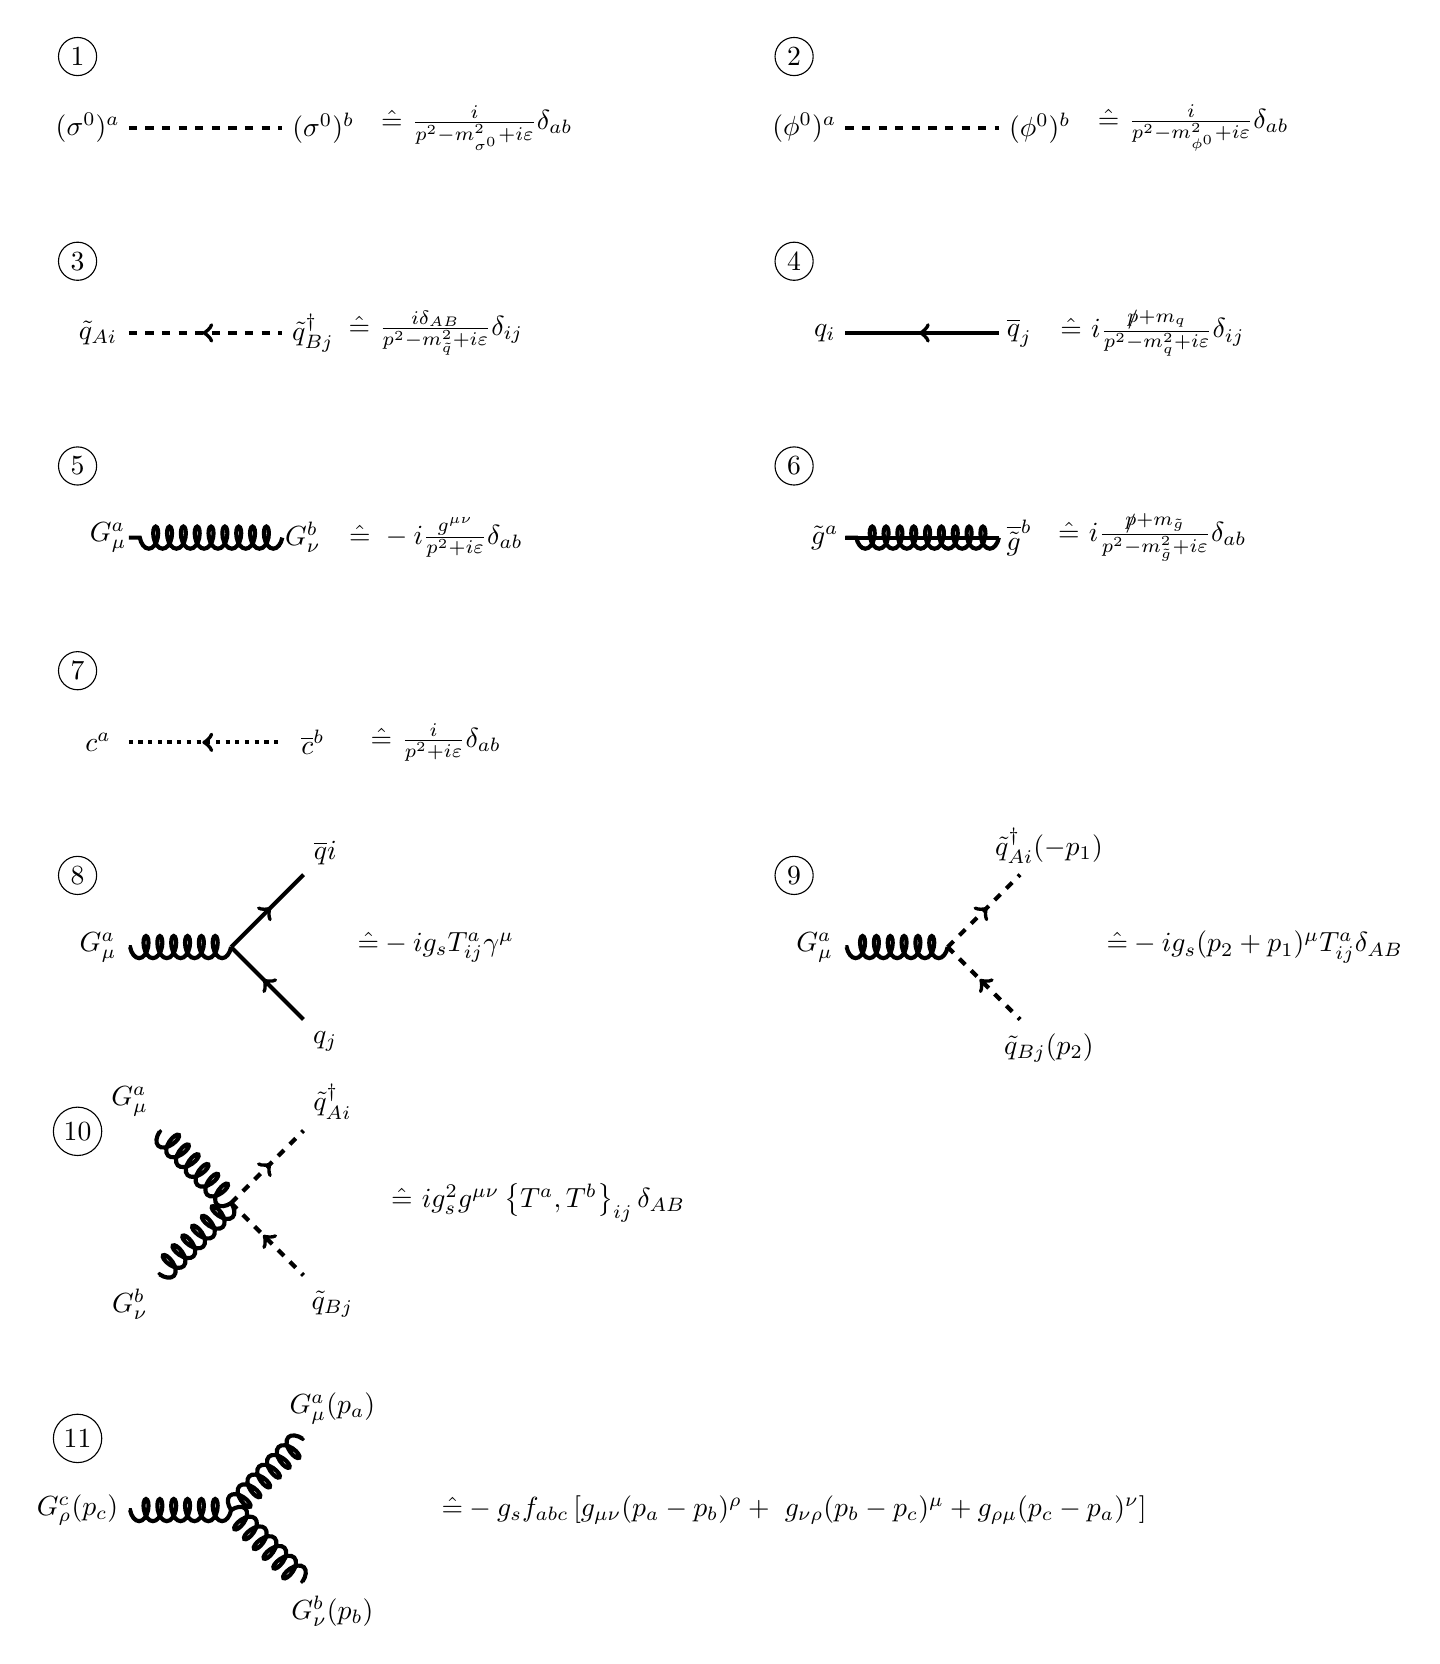
\begin{tikzpicture}[line width=1.5 pt, scale=1.3]
	\node at (-0.5,0.7) {\circled{1}};	
	\draw[scalarnoarrow](0,0)--(1.5,0);
	\node at (180:0.4) {$(\sigma^0)^a$};
	\node at (0:1.9) {$(\sigma^0)^b$};
	\node at (3.4,0) {$\hat{=}\ \frac{i}{p^2-m_{\sigma^0}^2+i\varepsilon}\delta_{ab}$};
\begin{scope}[shift={(7,0)}]
	\node at (-0.5,0.7) {\circled{2}};
	\draw[scalarnoarrow](0,0)--(1.5,0);
	\node at (180:0.4) {$(\phi^0)^a$};
	\node at (0:1.9) {$(\phi^0)^b$};
	\node at (3.4,0) {$\hat{=}\ \frac{i}{p^2-m_{\phi^0}^2+i\varepsilon}\delta_{ab}$};
\end{scope}
\begin{scope}[shift={(0,-2)}]
	\node at (-0.5,0.7) {\circled{3}};
	\draw[scalarbar](0,0)--(1.5,0);
	\node at (180:0.3) {$\tilde{q}_{Ai}$};
	\node at (0:1.8) {$\tilde{q}_{Bj}^\dagger$};
	\node at (3,0) {$\hat{=}\ \frac{i\delta_{AB}}{p^2-m_{\tilde{q}}^2+i\varepsilon}\delta_{ij}$};
\end{scope}
\begin{scope}[shift={(7,-2)}]
	\node at (-0.5,0.7) {\circled{4}};
	\draw[fermionbar](0,0)--(1.5,0);
	\node at (180:0.2) {$q_i$};
	\node at (0:1.7) {$\overline{q}_j$};
	\node at (3,0) {$\hat{=}\ i\frac{\slashed{p}+m_q}{p^2-m_q^2+i\varepsilon}\delta_{ij}$};
\end{scope}
\begin{scope}[shift={(0,-4)}]
	\draw[gluon](1.5,0)--(0,0);
	\node at (-0.5,0.7) {\circled{5}};
	\node at (180:0.2) {$G_\mu^a$};
	\node at (0:1.7) {$G_\nu^b$};
	\node at (3,0) {$\hat{=}\ -i\frac{g^{\mu\nu}}{p^2+i\varepsilon}\delta_{ab}$};
\end{scope}
\begin{scope}[shift={(7,-4)}]
	\node at (-0.5,0.7) {\circled{6}};
	\draw[gluon](1.5,0)--(0,0);
	\draw[fermionnoarrow](0,0)--(1.5,0);
	\node at (180:0.2) {$\tilde{g}^a$};
	\node at (0:1.7) {$\overline{\tilde{g}}^b$};
	\node at (3,0) {$\hat{=}\ i\frac{\slashed{p}+m_{\tilde{g}}}{p^2-m_{\tilde{g}}^2+i\varepsilon}\delta_{ab}$};
\end{scope}
\begin{scope}[shift={(0,-6)}]
	\node at (-0.5,0.7) {\circled{7}};
	\draw[ghostbar](0,0)--(1.5,0);
	\node at (180:0.3) {$c^{a}$};
	\node at (0:1.8) {$\overline{c}^{b}$};
	\node at (3,0) {$\hat{=}\ \frac{i}{p^2+i\varepsilon}\delta_{ab}$};
\end{scope}

\begin{scope}[shift={(1,-8)}]
	\node at (-1.5,0.7) {\circled{8}};
	\draw[fermion] (0,0)--(45:1);
	\draw[fermionbar] (0,0)--(-45:1);
	\draw[gluon] (0,0)--(180:1);
	\node at (45:1.3) {$\overline{q}i$};
	\node at (-45:1.3) {$q_j$};
	\node at (180:1.3) {$G_\mu^a$};
	\node at (2,0) {$\hat{=} -ig_s T^a_{ij}\gamma^\mu$};
\end{scope}
\begin{scope}[shift={(8,-8)}]
	\node at (-1.5,0.7) {\circled{9}};
	\draw[scalar] (0,0)--(45:1);
	\draw[scalarbar] (0,0)--(-45:1);
	\draw[gluon] (0,0)--(180:1);
	\node at (45:1.4) {$\tilde{q}^\dagger_{Ai}(-p_1)$};
	\node at (-45:1.4) {$\tilde{q}_{Bj}(p_2)$};
	\node at (180:1.3) {$G_\mu^a$};
	\node at (3,0) {$\hat{=} -ig_s (p_2+p_1)^\mu T^a_{ij}\delta_{AB}$};
\end{scope}
\begin{scope}[shift={(1,-10.5)}]
	\node at (-1.5,0.7) {\circled{10}};
	\draw[scalar] (0,0)--(45:1);
	\draw[scalarbar] (0,0)--(-45:1);
	\draw[gluon] (0,0)--(135:1);
	\draw[gluon] (0,0)--(-135:1);
	\node at (45:1.4) {$\tilde{q}^\dagger_{Ai}$};
	\node at (-45:1.4) {$\tilde{q}_{Bj}$};
	\node at (135:1.4) {$G_\mu^a$};
	\node at (-135:1.4) {$G_\nu^b$};
	\node at (3,0) {$\hat{=} \ ig_s^2 g^{\mu\nu} \left\{T^a,T^b\right\}_{ij}\delta_{AB}$};
\end{scope}
\begin{scope}[shift={(1,-13.5)}]
	\node at (-1.5,0.7) {\circled{11}};
	\draw[gluon] (0,0)--(45:1);
	\draw[gluon] (0,0)--(-45:1);
	\draw[gluon] (0,0)--(180:1);
	\node at (45:1.4) {$G_\mu^a(p_a)$};
	\node at (-45:1.4) {$G_\nu^b(p_b)$};
	\node at (180:1.5) {$G_\rho^c(p_c)$};
	\node at (5.5,0) {$\hat{=}  - g_s f_{abc} \left[ g_{\mu\nu}(p_a-p_b)^\rho +\  g_{\nu\rho}(p_b-p_c)^\mu +  g_{\rho\mu}(p_c-p_a)^\nu \right]$};
\end{scope}
\end{tikzpicture}
\caption{In the Feynman diagrams of the propagators the momentum is flowing from the right to the left hand side. The gluon propagator is given in Feynman gauge.\newline
In the Feynman diagrams of the vertices all momenta flow towards the vertex, i.e. in diagram 9 $-p_1$ is flowing towards the vertex.\newline
The indices $A,B \in \left\{ L,R \right\}$ label the left/right ``handedness'' of the squarks. The indices $i,j=1,2,3$ are the color indices in the (anti)fundamental representation where $a,b,c,\hdots = 1,\hdots,8$ are the color indices of the adjoint representation.}\label{fig:firstFeynmanRules}
\end{center}
\end{figure}
\newpage

%The gluino-quark-squark vertex is not much different from the one in SQCD. One only must avoid replacing $\tilde{g}$ with $\tilde{g}^C$. %See for the derivation of Feynman rules for theories with fermion number violating interaction reference [a. denner, h.eck, o. hahn, j. küblbeck]
\begin{figure}[H]
\begin{center}
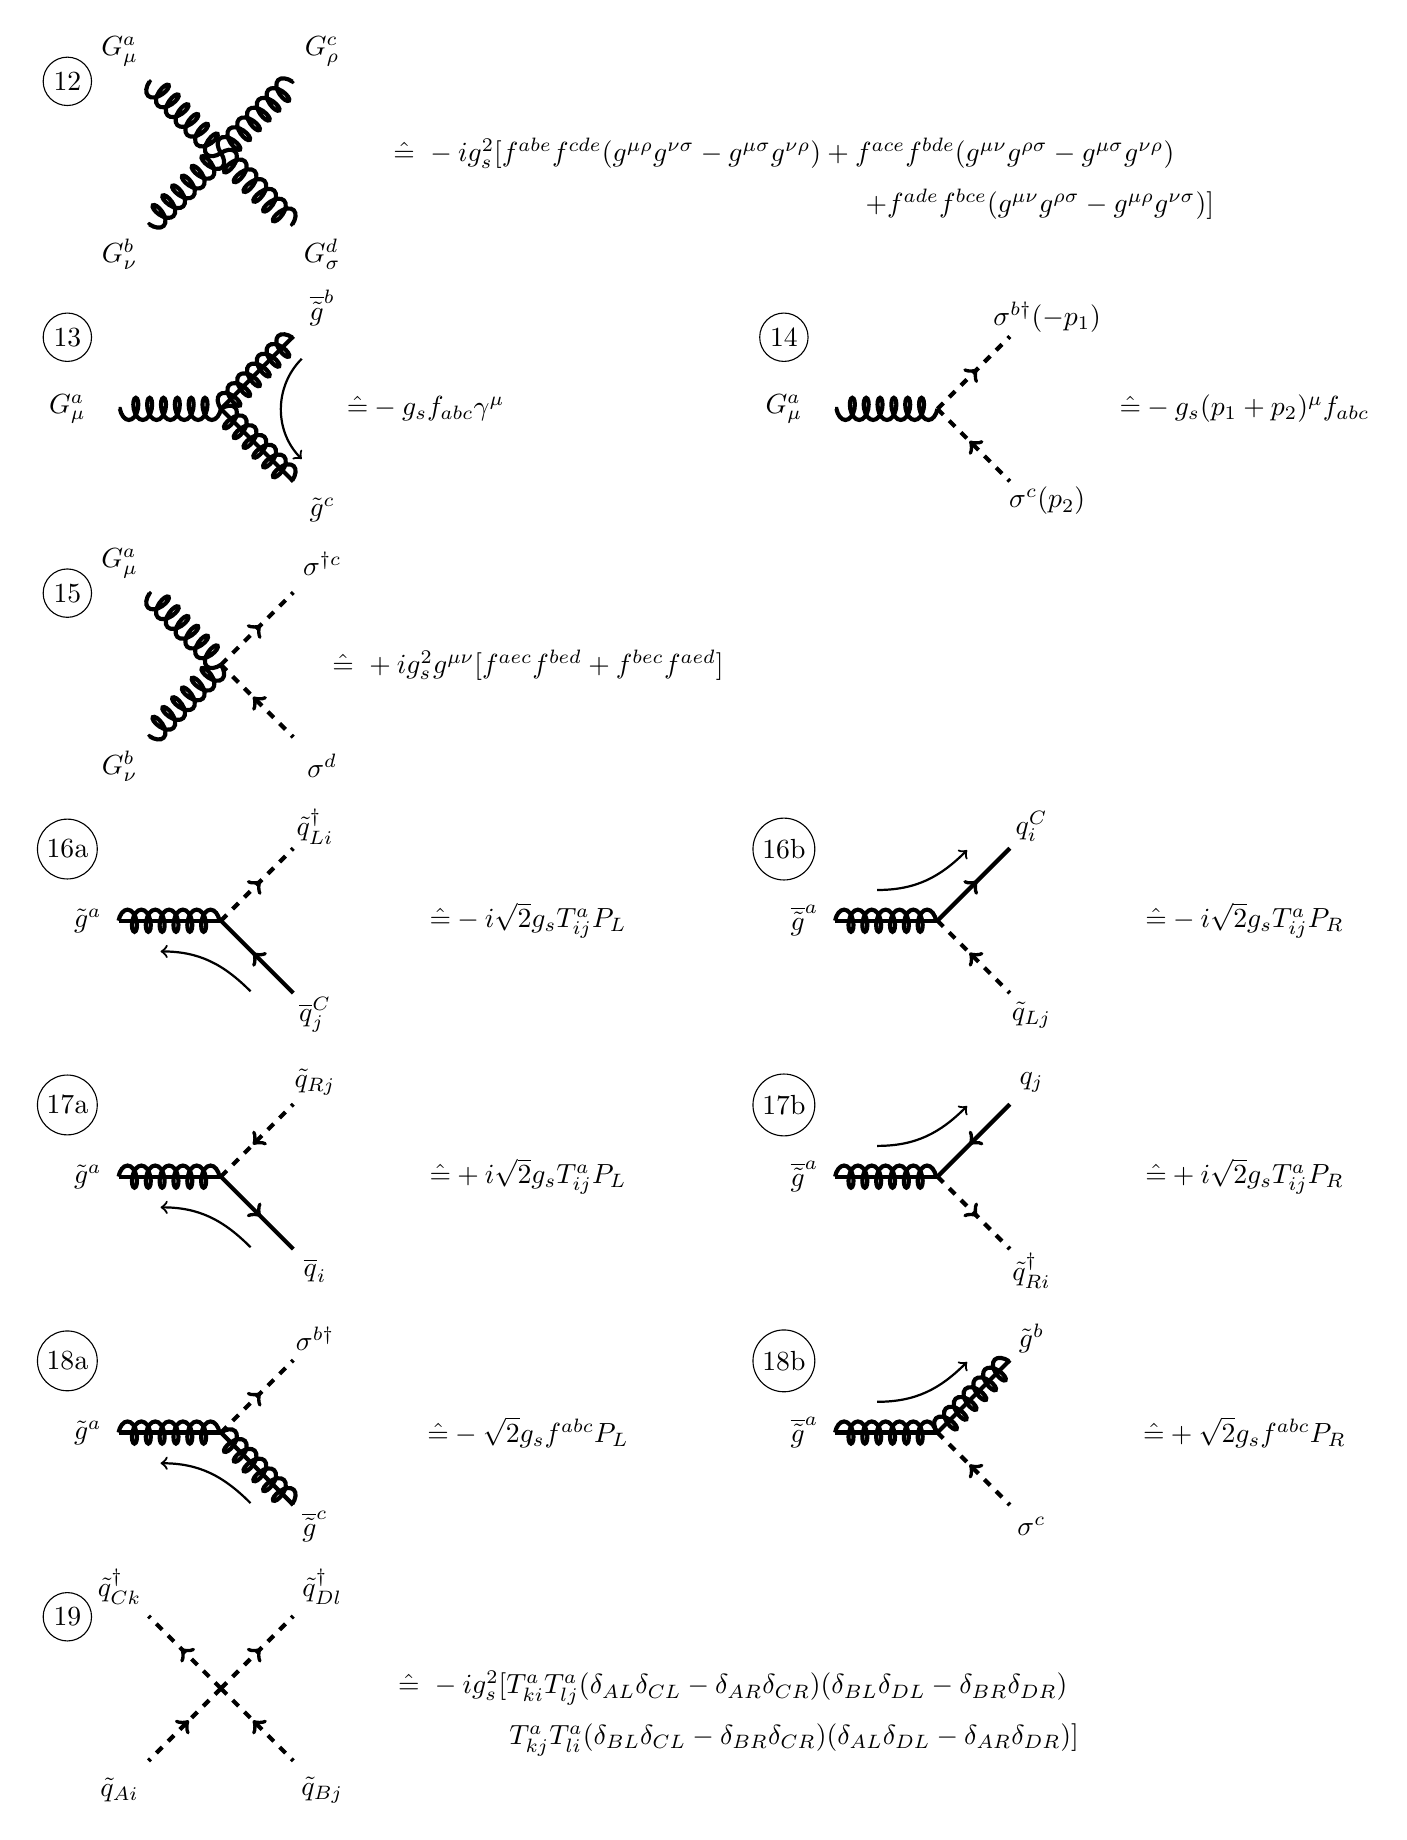
\begin{tikzpicture}[line width=1.5 pt, scale=1.3]
	\node at (-1.5,0.7) {\circled{12}};
	\draw[gluon] (0,0)--(45:1);
	\draw[gluon] (0,0)--(-45:1);
	\draw[gluon] (0,0)--(135:1);
	\draw[gluon] (0,0)--(-135:1);
	\node at (45:1.4) {$G_\rho^c$};
	\node at (-45:1.4) {$G_\sigma^d$};
	\node at (135:1.4) {$G_\mu^a$};
	\node at (-135:1.4) {$G_\nu^b$};
	\node at (5.5,0) {$\hat{=} \ -ig_s^2 [f^{abe}f^{cde}(g^{\mu\rho} g^{\nu\sigma} - g^{\mu\sigma}g^{\nu\rho}) + f^{ace}f^{bde}(g^{\mu\nu} g^{\rho\sigma} - g^{\mu\sigma}g^{\nu\rho}) $};
	\node at (8,-0.5) {$+ f^{ade}f^{bce}(g^{\mu\nu} g^{\rho\sigma} - g^{\mu\rho}g^{\nu\sigma})]$};
\begin{scope}[shift={(0,-2.5)}]
	\node at (-1.5,0.7) {\circled{13}};
	\draw[gluon] (0,0)--(180:1);
	\draw[gluon] (0,0)--(45:1);
	\draw[gluon] (0,0)--(-45:1);
	\draw[fermionnoarrow] (0,0)--(-45:1);
	\draw[fermionnoarrow] (0,0)--(45:1);
	\node at (45:1.4) {$\overline{\tilde{g}}^b$};
	\node at (-45:1.4) {$\tilde{g}^c$};
	\node at (180:1.5) {$G_\mu^a$};
	\node(gbar) at (0.9,0.6) {};
	\node(g) at (0.9,-0.6) {};
	\path[line width=0.8pt,<-] (g) edge [out=135, in=-135] (gbar);
	\node at (2,0) {$\hat{=}  - g_s f_{abc} \gamma^\mu$};
\end{scope}
\begin{scope}[shift={(7,-2.5)}]
	\node at (-1.5,0.7) {\circled{14}};
	\draw[gluon] (0,0)--(180:1);
	\draw[scalar] (0,0)--(45:1);
	\draw[scalarbar] (0,0)--(-45:1);
	\node at (40:1.4) {$\sigma^{b\dagger}(-p_1)$};
	\node at (-40:1.4) {$\sigma^c(p_2)$};
	\node at (180:1.5) {$G_\mu^a$};
	\node at (3,0) {$\hat{=}  - g_s (p_1+p_2)^\mu f_{abc} $};
\end{scope}
\begin{scope}[shift={(0,-5)}]
	\node at (-1.5,0.7) {\circled{15}};
	\draw[scalar] (0,0)--(45:1);
	\draw[scalarbar] (0,0)--(-45:1);
	\draw[gluon] (0,0)--(135:1);
	\draw[gluon] (0,0)--(-135:1);
	\node at (45:1.4) {$\sigma^{\dagger c}$};
	\node at (-45:1.4) {$\sigma^d$};
	\node at (135:1.4) {$G_\mu^a$};
	\node at (-135:1.4) {$G_\nu^b$};
	\node at (3,0) {$\hat{=} \ +ig_s^2 g^{\mu\nu}[f^{aec}f^{bed}+ f^{bec}f^{aed}]$};
\end{scope}
\begin{scope}[shift={(0,-7.5)}]
	\node at (-1.5,0.7) {\circled{16a}};
	\draw[scalar] (0,0)--(45:1);
	\draw[fermionbar] (0,0)--(-45:1);
	\draw[fermionnoarrow] (180:1)--(0,0);
	\draw[gluon] (180:1)--(0,0);
	\node at (45:1.3) {$\tilde{q}_{Li}^\dagger$};
	\node at (-45:1.3) {$\overline{q}^C_j$};
	\node at (180:1.3) {$\tilde{g}^a$};
	\node(g) at (-0.7,-0.3) {};
	\node(u) at (0.4,-0.8) {};
	\path[line width=0.8pt,<-] (g) edge [out=0, in=135] (u);
	\node at (3,0) {$\hat{=} -i\sqrt{2}g_s T^a_{ij}P_L$};
\end{scope}
\begin{scope}[shift={(7,-7.5)}]
	\node at (-1.5,0.7) {\circled{16b}};
	\draw[fermion] (0,0)--(45:1);
	\draw[scalarbar] (0,0)--(-45:1);
	\draw[fermionnoarrow] (180:1)--(0,0);
	\draw[gluon] (180:1)--(0,0);
	\node at (45:1.3) {$q^C_i$};
	\node at (-45:1.3) {$\tilde{q}_{Lj}$};
	\node at (180:1.3) {$\overline{\tilde{g}}^a$};
	\node(g) at (-0.7,0.3) {};
	\node(u) at (0.4,0.8) {};
	\path[line width=0.8pt,->] (g) edge [out=0, in=225] (u);
	\node at (3,0) {$\hat{=} -i\sqrt{2}g_s T^a_{ij}P_R$};
\end{scope}
\begin{scope}[shift={(0,-10)}]
	\node at (-1.5,0.7) {\circled{17a}};
	\draw[scalarbar] (0,0)--(45:1);
	\draw[fermion] (0,0)--(-45:1);
	\draw[fermionnoarrow] (180:1)--(0,0);
	\draw[gluon] (180:1)--(0,0);
	\node at (45:1.3) {$\tilde{q}_{Rj}$};
	\node at (-45:1.3) {$\overline{q}_i$};
	\node at (180:1.3) {$\tilde{g}^a$};
	\node(g) at (-0.7,-0.3) {};
	\node(u) at (0.4,-0.8) {};
	\path[line width=0.8pt,<-] (g) edge [out=0, in=135] (u);
	\node at (3,0) {$\hat{=} +i\sqrt{2}g_s T^a_{ij}P_L$};
\end{scope}
\begin{scope}[shift={(7,-10)}]
	\node at (-1.5,0.7) {\circled{17b}};
	\draw[fermionbar] (0,0)--(45:1);
	\draw[scalar] (0,0)--(-45:1);
	\draw[fermionnoarrow] (180:1)--(0,0);
	\draw[gluon] (180:1)--(0,0);
	\node at (45:1.3) {$q_j$};
	\node at (-45:1.3) {$\tilde{q}_{Ri}^\dagger$};
	\node at (180:1.3) {$\overline{\tilde{g}}^a$};
	\node(g) at (-0.7,0.3) {};
	\node(u) at (0.4,0.8) {};
	\path[line width=0.8pt,->] (g) edge [out=0, in=225] (u);
	\node at (3,0) {$\hat{=} +i\sqrt{2}g_s T^a_{ij}P_R$};
\end{scope}
\begin{scope}[shift={(0,-12.5)}]
	\node at (-1.5,0.7) {\circled{18a}};
	\draw[scalar] (0,0)--(45:1);
	\draw[fermionnoarrow] (0,0)--(-45:1);
	\draw[gluon] (0,0)--(-45:1);
	\draw[fermionnoarrow] (180:1)--(0,0);
	\draw[gluon] (180:1)--(0,0);
	\node at (45:1.3) {$\sigma^{b\dagger}$};
	\node at (-45:1.3) {$\overline{\tilde{g}}^c$};
	\node at (180:1.3) {$\tilde{g}^a$};
	\node(g) at (-0.7,-0.3) {};
	\node(u) at (0.4,-0.8) {};
	\path[line width=0.8pt,<-] (g) edge [out=0, in=135] (u);
	\node at (3,0) {$\hat{=} -\sqrt{2}g_s f^{abc}P_L$};
\end{scope}
\begin{scope}[shift={(7,-12.5)}]
	\node at (-1.5,0.7) {\circled{18b}};
	\draw[fermionnoarrow] (0,0)--(45:1);
	\draw[gluon] (0,0)--(45:1);
	\draw[scalarbar] (0,0)--(-45:1);
	\draw[fermionnoarrow] (180:1)--(0,0);
	\draw[gluon] (180:1)--(0,0);
	\node at (45:1.3) {$\tilde{g}^b$};
	\node at (-45:1.3) {$\sigma^c$};
	\node at (180:1.3) {$\overline{\tilde{g}}^a$};
	\node(g) at (-0.7,0.3) {};
	\node(u) at (0.4,0.8) {};
	\path[line width=0.8pt,->] (g) edge [out=0, in=225] (u);
	\node at (3,0) {$\hat{=} +\sqrt{2}g_s f^{abc} P_R$};
\end{scope}
\begin{scope}[shift={(0,-15)}]
	\node at (-1.5,0.7) {\circled{19}};
	\draw[scalar] (0,0)--(45:1);
	\draw[scalarbar] (0,0)--(-45:1);
	\draw[scalar] (0,0)--(135:1);
	\draw[scalarbar] (0,0)--(-135:1);
	\node at (45:1.4) {$\tilde{q}^\dagger_{Dl}$};
	\node at (-45:1.4) {$\tilde{q}_{Bj}$};
	\node at (135:1.4) {$\tilde{q}^\dagger_{Ck}$};
	\node at (-135:1.4) {$\tilde{q}_{Ai}$};
	\node at (5,0) {$\hat{=} \ -ig_s^2 [T_{ki}^a T_{lj}^a(\delta_{AL}\delta_{CL} - \delta_{AR}\delta_{CR})(\delta_{BL}\delta_{DL}-\delta_{BR}\delta_{DR})$};
	\node at (5.6,-0.5) {$T_{kj}^a T_{li}^a(\delta_{BL}\delta_{CL} - \delta_{BR}\delta_{CR})(\delta_{AL}\delta_{DL}-\delta_{AR}\delta_{DR})]$};
\end{scope}
\end{tikzpicture}
\end{center}
\caption{The curved arrows indicate the fermion flow. The Feynman rules 16b, 17b and 18b are the complex conjugates of 16a, 17a and 18a respectively. Applying a flipping rule to a vertex one has to reverse the curved arrow, i.e. the fermion flow and replace $\Psi$ with $\bar{\Psi}^C$. In addition one has to add a minus sign for Feynman rule 13.}\label{fig:secondFeynmanRules}
\end{figure}
\begin{figure}[H]
\begin{center}
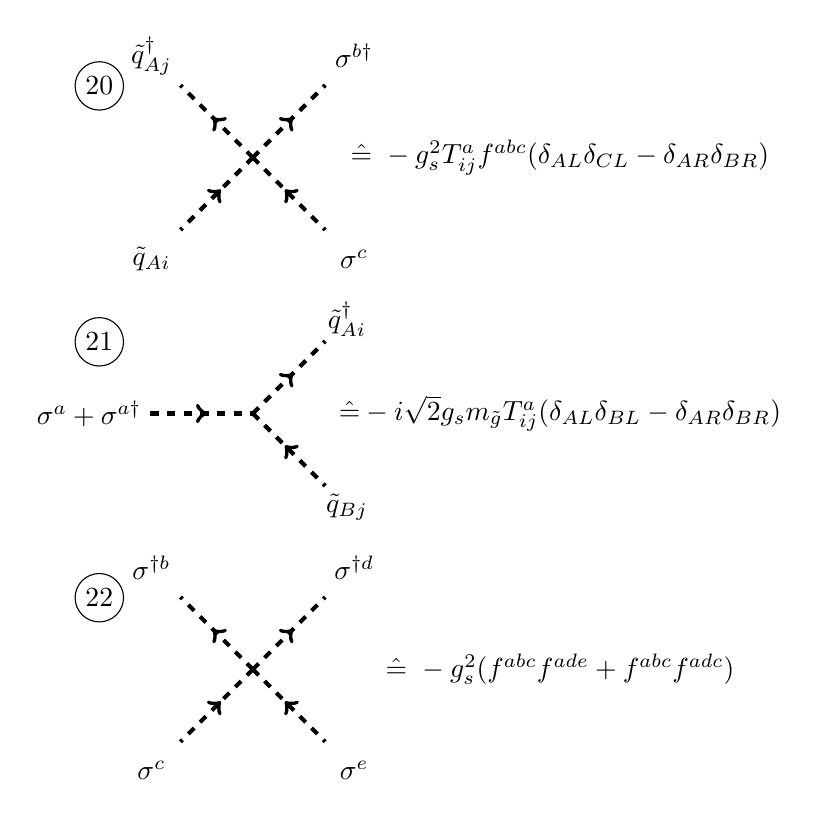
\begin{tikzpicture}[line width=1.5 pt, scale=1.3]
	\node at (-1.5,0.7) {\circled{20}};
	\draw[scalar] (0,0)--(45:1);
	\draw[scalarbar] (0,0)--(-45:1);
	\draw[scalar] (0,0)--(135:1);
	\draw[scalarbar] (0,0)--(-135:1);
	\node at (45:1.4) {$\sigma^{b\dagger}$};
	\node at (-45:1.4) {$\sigma^c$};
	\node at (135:1.4) {$\tilde{q}^\dagger_{Aj}$};
	\node at (-135:1.4) {$\tilde{q}_{Ai}$};
	\node at (3,0) {$\hat{=} \ -g_s^2 T_{ij}^a f^{abc}(\delta_{AL}\delta_{CL} - \delta_{AR}\delta_{BR})$};
\begin{scope}[shift={(0,-2.5)}]
	\node at (-1.5,0.7) {\circled{21}};
	\draw[scalar] (0,0)--(45:1);
	\draw[scalarbar] (0,0)--(-45:1);
	\draw[scalar] (180:1)--(0,0);
	\node at (45:1.3) {$\tilde{q}^\dagger_{Ai}$};
	\node at (-45:1.3) {$\tilde{q}_{Bj}$};
	\node at (180:1.6) {$\sigma^a+\sigma^{a\dagger}$};
	\node at (3,0) {$\hat{=} -i\sqrt{2}g_s m_{\tilde{g}} T^a_{ij}(\delta_{AL}\delta_{BL}-\delta_{AR}\delta_{BR})$};
\end{scope}
\begin{scope}[shift={(0,-5)}]
	\node at (-1.5,0.7) {\circled{22}};
	\draw[scalar] (0,0)--(45:1);
	\draw[scalarbar] (0,0)--(-45:1);
	\draw[scalar] (0,0)--(135:1);
	\draw[scalarbar] (0,0)--(-135:1);
	\node at (45:1.4) {$\sigma^{\dagger d}$};
	\node at (-45:1.4) {$\sigma^e$};
	\node at (135:1.4) {$\sigma^{\dagger b}$};
	\node at (-135:1.4) {$\sigma^c$};
	\node at (3,0) {$\hat{=} \ -g_s^2 (f^{abc}f^{ade} + f^{abc}f^{adc})$};
\end{scope}
\end{tikzpicture}
\end{center}
\end{figure}


\subsection{Passarino-Veltman Integrals}\label{sec:Passarino}
The definition of the momenta within the Passarino-Veltman integrals in this thesis agrees with the one from \texttt{Looptools} \cite{Hahn:1998} convention. The original paper \cite{Passarino:1978jh} uses slightly different conventions. A pedagogical introduction to the evaluation of one-loop integrals can be found in \cite{Ellis:2011cr}.  $A$, $B$ and $C$ integrals are defined by:
\begin{align}
\frac{i}{16\pi^2} A_0(m^2) &= \int_l \frac{1}{l^2-m^2}\nonumber\\
\frac{i}{16\pi^2} B_{0,\mu,\mu\nu}(p^2,m_1^2,m_2^2) &= \int_l \frac{\left\{1,l_\mu,l_\mu l_\nu \right\}}{[l^2-m_1^2][(l+p)^2-m_2^2]}\\
\frac{i}{16\pi^2} C_{0,\mu,\mu\nu}(p_1^2,p_2^2,(p_1+p_2)^2,m_1^2,m_2^2,m_3^2) &= \int_l \frac{\left\{1,l_\mu,l_\mu l_\nu \right\}}{[l^2-m_1^2][(l+p_1)^2-m_2^2][(l+p_1+p_2)^2-m_3^2]}.\nonumber\label{eq:LoopInt}
\end{align}
with the shortcut $\int_l = \mu^{2\epsilon}\int\frac{\mathrm{d}^D l}{(2\pi)^D}$. Furthermore there are supressed $\varepsilon$'s which prescripe how the poles in the complex plane are avoided. They are hidden in the infinitesimal shift of the masses: $m_i^2 \to m_i^2 - i \varepsilon$.\\
The tensor integrals can be decomposed as
\begin{align}
B_\mu &:= p_\mu B_1\nonumber\\
B_{\mu\nu} &:= g_{\mu\nu}B_{00} + p_\mu p_\nu B_{11}\nonumber\\
C_\mu &= p_{1\mu}C_1 + p_{2\mu}C_2\\
C_{\mu\nu} &:= g_{\mu\nu}C_{00} + p_{1\mu}p_{1\nu}C_{11} + p_{2\mu}p_{2\nu}C_{22} + (p_{1\mu}p_{2\nu} + p_{2\mu}p_{1\nu})C_{12}\nonumber
\end{align}
In the the special case of vanishing momenta the integrals take a succinct form. %The following formulae show some of these special cases.
\begin{align}
A_0(m^2) = m^2\left( \Delta_\epsilon -\ln \frac{m^2}{\mu^2} + 1 \right) + \mathcal{O}(\epsilon)
\end{align}
where the typical UV-divergent constant $\Delta_\epsilon = \frac{1}{\epsilon} - \gamma_E+\ln 4\pi$ is defined. It comprises the Euler-Mascheroni constant $\gamma_{\mathrm{E}}$.
\begin{align}
B_0(0,m_1^2,m_2^2) &= \frac{A_0(m_1^2)-A_0(m_2^2)}{m_1^2-m_2^2} = \Delta_\epsilon + 1 -\frac{m_1^2\ln \frac{m_1^2}{\mu^2}-m_2^2\ln \frac{m_2^2}{\mu^2}}{m_1^2-m_2^2} + \mathcal{O}(\epsilon)\\
B_0(0,m^2,m^2) &= \frac{\partial}{\partial m^2} A_0(m^2) = \Delta_\epsilon -\ln \frac{m^2}{\mu^2} + \mathcal{O}(\epsilon)\\
B_0(0,0,0) &= 0\\
B_1(0,m_1^2,m_2^2) &= -\frac{\Delta_\epsilon}{2} + \frac{1}{2}\ln \frac{m_1^2}{\mu^2} + \frac{-3+4t-t^2-4t \ln t +2t^2 \ln t}{4(t-1)^2} + \mathcal{O}(\epsilon)\label{eq:B1}\\
B_1(0,0,0) &= 0
\end{align}
The scaleless integrals are defined to be zero due to their definition  on how they scale in $D$ dimensions\cite{Collins:105730}. The parameter $t$ is given by $\frac{m_2^2}{m_1^2}$. As can be seen from \ref{eq:B1} $B_1$ is in contrast to $B_0$ not symmetric in its masses but it can be shown [Romao] that
\begin{align}
B_1(p^2,m_1^2,m_2^2) = -(B_0(p^2,m_2^2,m_1^2) + B_1(p^2,m_2^2,m_1^2))
\end{align}
It can further be shown that
\begin{align}
C_{00}(0,0,0,m_1^2, m_1^2, m_2^2) = -\frac{1}{2}B_1(0, m_1^2, m_2^2)
\end{align} and that $C_{00}(0,0,0,m_1^2, m_1^2, m_2^2)$ is a symmetric function of its masses.\\
From the generic $\epsilon$-expansion of the $B_0$ integral \cite{Denner}
\begin{align}
B_0(p^2,m_1^2,m_2^2) = \Delta_\epsilon - \int_0^1\mathrm{d}x\ \ln \frac{-x(1-x)p^2 + xm_2^2 + (1-x)m_1^2}{\mu^2}
\end{align} 
and Passarino-Veltman decomposition \cite{Passarino:1978jh} one can determine the UV-divergent part of all $B$ and $C$ integrals. In chapter \ref{sec:MSRen} this was necessary in order to obtain the renormalization constants in the $\overline{\mathrm{MS}}$-scheme. Infrared and collinear singularities arise from the special case where one or multiple masses tend to zero. These poles can be regularized with a small mass cutoff $\Lambda$ leading singularities of the form $\ln \Lambda$ or dimensionally which leads to $\epsilon$-poles as in the treatment of UV-divergences. In the latter case the integral first needs to undergo the limit to zero masses and than being evaluated.\\
The following list shows all necessary integrals needed to determine the renormalization constants in \ref{sec:MSRen}.
\begin{align}
\left.A_0(m^2)\right|_{\mathrm{UV-div}} &= m^2 \Delta_\epsilon\\
\left.B_0(p^2,m_1^2,m_2^2)\right|_{\mathrm{UV-div}} &= \Delta_\epsilon\\
\left.B_1(p^2,m_1^2,m_2^2)\right|_{\mathrm{UV-div}} &= -\frac{1}{2}\Delta_\epsilon\\
\left.C_{00}(p_1^2,p_2^2,(p_1+p_2)^2,m_1^2,m_2^2,m_3^2)\right|_{\mathrm{UV-div}} &= \frac{1}{4}\Delta_\epsilon
\end{align}
The UV-divergent part of $C_{11}$, $C_{22}$, $C_{12}$ equals zero. As can be seen already from the superficial degree of divergence also $C_i|_{\mathrm{UV-div}} = 0$ for $i \in \left\{ 0, 1, 2 \right\}$ .



\subsection{Cross section and Phase Space Integration}\label{sec:cross_section}
Once the Feynman amplitude $\mathcal{M}$ for a $2 \to N$ body scattering\footnote{with kinematics $k_a + k_b \to p_1 + \hdots p_N$} is computed one can calculate physical observables with it. The differential cross section for $2 \to N$ scattering is given by
\begin{align}
\mbox{d}\sigma = \frac{1}{F}\mathrm{d}\Phi_N |\mathcal{M}|^2.
\end{align}
The flux factor is defined by $F = 4\sqrt{(k_a\cdot k_b)^2 - (m_am_b)^2}$ which equals $F = 2s$ for massless initial state particles. The differential for the $N$ body phase space in $D$ dimensions is given by
\begin{align}
\mathrm{d}\Phi_N = \left( \mu^{2\epsilon} \right)^{N-1} \left( \prod_{f=1}^N \frac{\mbox{d}^{D-1}p_f}{(2\pi)^{D-1}}\frac{1}{2E_f} \right)  (2\pi)^D \delta^{(D)}(k_a+k_b-\sum_{f=1}^N p_f).
\end{align} 
The factor $\mu^{2\epsilon}$ is included to maintain the mass dimension of the cross section. As in this thesis the sum of $|\mathcal{M}|^2$ over helicities and colors $\sum |\mathcal{M}|^2$ has been calculated one can write
\begin{align}
\mathrm{d}\sigma = \frac{1}{2s} \mathrm{d}\Phi_2 K_{ab} \sum |\mathcal{M}|^2
\end{align} 
where $K_{ab}$ encodes the averaging over initial state helicities and colors. Specifying to the center-of-mass frame and assuming that $\sum|\mathcal{M}|^2$ is only a function of the modulus of one of the final state particle's 3-momentum $ |\vec{p}_i|$ and the angle $\theta$ between $\vec{k}_a$ and $\vec{p}_1$ one can write
\begin{align}
\int \mathrm{d}\Phi_2 &= \mu^{2\epsilon} \int \frac{\mathrm{d}|\vec{p}_1|\mathrm{d}\Omega^{D-1}_1}{(2\pi)^{D-2} 4 E_1 E_2} |\vec{p}_1|^{D-2} \delta \left(k_a^0 + k_b^0 - \sqrt{m_1^2 + |\vec{p}_1|^2} - \sqrt{m_2^2 + |\vec{p}_1|^2} \right)\nonumber\\
&= \frac{1}{(2\pi)^{D-2}}\frac{2\pi^{\frac{D}{2}-1}}{\Gamma(\frac{D}{2}-1)} \mu^{2\epsilon} \int_0^\infty\mathrm{d}|\vec{p}_1| \int_0^\pi \mathrm{d} \cos\theta \frac{1}{4 E_1 E_2} p_1^{D-2}\sin^{D-4}\theta\nonumber\\
&\ \ \delta \left(k_a^0 + k_b^0 - \sqrt{m_1^2 + |\vec{p}_1|^2} - \sqrt{m_2^2 + |\vec{p}_1|^2} \right).\label{eq:DPhi2}
\end{align}
In the second line the integral over the D-dimensional hypersphere 
\begin{align}
\int \mathrm{d}\Omega^D = \int_0^{2\pi} \mathrm{d}\phi \prod_{i=1}^{D-2}\int_0^\pi \sin^i\theta_i \mathrm{d}\theta_i = \frac{2\pi^{\frac{D}{2}}}{\Gamma(\frac{D}{2})}
\end{align}
has been used. Because $\sum|\mathcal{M}|^2$ is calculated in terms of Mandelstam variables 
\begin{align}
t &= (k_a-p_1)^2  \nonumber\\
t &= -2\left(|\vec{k}_a| \sqrt{m_1^2 + |\vec{p}_1|^2} - |\vec{k}_a||\vec{p}_1| \cos\theta\right) + m_1^2\label{eq:t} \\
u &= (k_a-p_2)^2\nonumber\\
u &= -2\left(|\vec{k}_a| \sqrt{m_2^2 + |\vec{p}_1|^2} + |\vec{k}_a||\vec{p}_1| \cos\theta\right) + m_2^2\label{eq:u}
\end{align}
it is useful to perform a change of coordinates yielding
\begin{align}
\mathrm{d}|\vec{p}_1|\ \mathrm{d}\cos\theta = -\frac{E_1 E_2}{4|\vec{k}_a|^2|\vec{p}_1|^2(E_1+E_2)}\mathrm{d}u\ \mathrm{d}t.\label{eq:PhaseTrafo}
\end{align}
Inserting \ref{eq:PhaseTrafo} into \ref{eq:DPhi2} and using $2|\vec{k}_a| = \sqrt{s} = E_1 + E_2$ gives
\begin{align}
\int \mathrm{d}\Phi_2 = & \frac{1}{s} \frac{\pi^{-\frac{D}{2}+1}}{2^{D-3}\Gamma(\frac{D}{2}-1)} \int \mathrm{d}u\ \mathrm{d}t\ \left( \frac{tu-m_1^2m_2^2}{\mu^{2\epsilon} s} \right)^{\frac{D-4}{2}} \nonumber\\
&\frac{1}{4}\Theta(tu-4m_1^2m_2^2)\delta \left(s+t+u-m_1^2-m_2^2\right)
\end{align}
where the $\Theta$-function comes from the bounds of $|\vec{p}_1|$ and $\theta$ visible in \ref{eq:DPhi2} and the combination of \ref{eq:t} and \ref{eq:u}. Working in $D=4-2\epsilon$ dimensions and inserting $\Theta(s-4m^2)$ with $m = \frac{m_1 + m_2}{2}$ to account for the production threshold one finds
\begin{align}
\frac{\mbox{d}^2 \sigma}{\mbox{d}t\mbox{d}u} =& \frac{K_{ab}}{s^2} \frac{\pi S_{\epsilon}}{\Gamma(1-\epsilon)} \left[ \frac{tu-m_1^2m_2^2}{\mu^2 s}\right]^{-\epsilon} \Theta(tu-m_1^2m_2^2)\nonumber\\
&\ \Theta(s-4m^2) \delta(s+t+u-m_1^2-m_2^2) \sum |\mathcal{M}|^2
\end{align}
where $S_\epsilon = (4\pi)^{-2+\epsilon}$ as defined in \cite{Beenakker:1996ch}.
The averaging factors $K_{ab}$ are given by
\begin{align}
K_{qq} = \frac{1}{4N_c^2} \hspace{1.5cm}K_{GG} = \frac{1}{4(1-\epsilon)^2(N_c^2-1)^2} \hspace{1.5cm}K_{qG} = \frac{1}{4(1-\epsilon)N_c(N_c^2-1)}.
\end{align}


\newpage
\bibliography{references}
\newpage
% Erklärung
\clearpage
\thispagestyle{empty}
\minisec{Erklärung}\vspace*{1.5em}
Hiermit erkläre ich, dass ich diese Arbeit im Rahmen der Betreuung am Institut
für ??? Physik ohne unzulässige Hilfe Dritter verfasst und alle Quellen als solche gekennzeichnet habe.
\vspace*{45em}
Vorname Nachname \par
Dresden, Monat 2012

\end{document}
